\chapter{Alternative Fit Studies}

A number of compatibility studies were performed, comparing subsets of data and using alternative fit models.

The data-subset results presented here were not used in the full oscillation analysis, but are part of the validations of the input models and fitting framework. The alternative model fits were used to inform choices in the interaction model used for the final fits.

These fits were all run using the uniform-rectangular fit binning and 574 merged detector bins.

\section{FGD1 and FGD2 Only Fits}

As discussed in Section \ref{sec:fgd}, FGD1 and FGD2 have different target materials. FGD2 has water layers, and so contains a significant amount of $^{16}$O, whereas FGD1 has only plastic scintillator (C$_8$H$_8$) layers. The constraint on $^{16}$O only parameters therefore comes only from FGD2. 

The location of the FGDs also causes differences in reconstruction between the two subdetectors. FGD1 has two TPCs downstream of it, and so performs more accurate reconstruction for forward-going tracks, whereas FGD2 has two TPCs upstream of it, and so performs more accurate reconstruction for backward going-tracks.

To investigate the compatibility of the FGD1 and FGD2 samples, fits were run using each independently. There is approximately the same amount of data in the FGD1 and FGD2 sample, so the constraining power of each is expected to be similar.

The results for the flux parameters are shown in Figures \ref{fig:fgdfluxND} and \ref{fig:fgdfluxSK}, along with the full FGD1 and FGD2 fit. The postfit values of the FGD1 and FGD2 only fits are consistently within the postfit uncertainties of both each other, and the full fit. The high pulls at lower energies are seen in all fits. The gradient of the decrease in pull with increasing energy shows some small discrepancies, but this is to be expected given the high correlations between the flux parameters.

The \SK flux parameters have very similar behaviour to the ND flux parameters, as is expected as they are only constrained by their prior correlations.

\begin{figure}
\centering
\begin{subfigure}{0.3\textwidth}
  \centering
  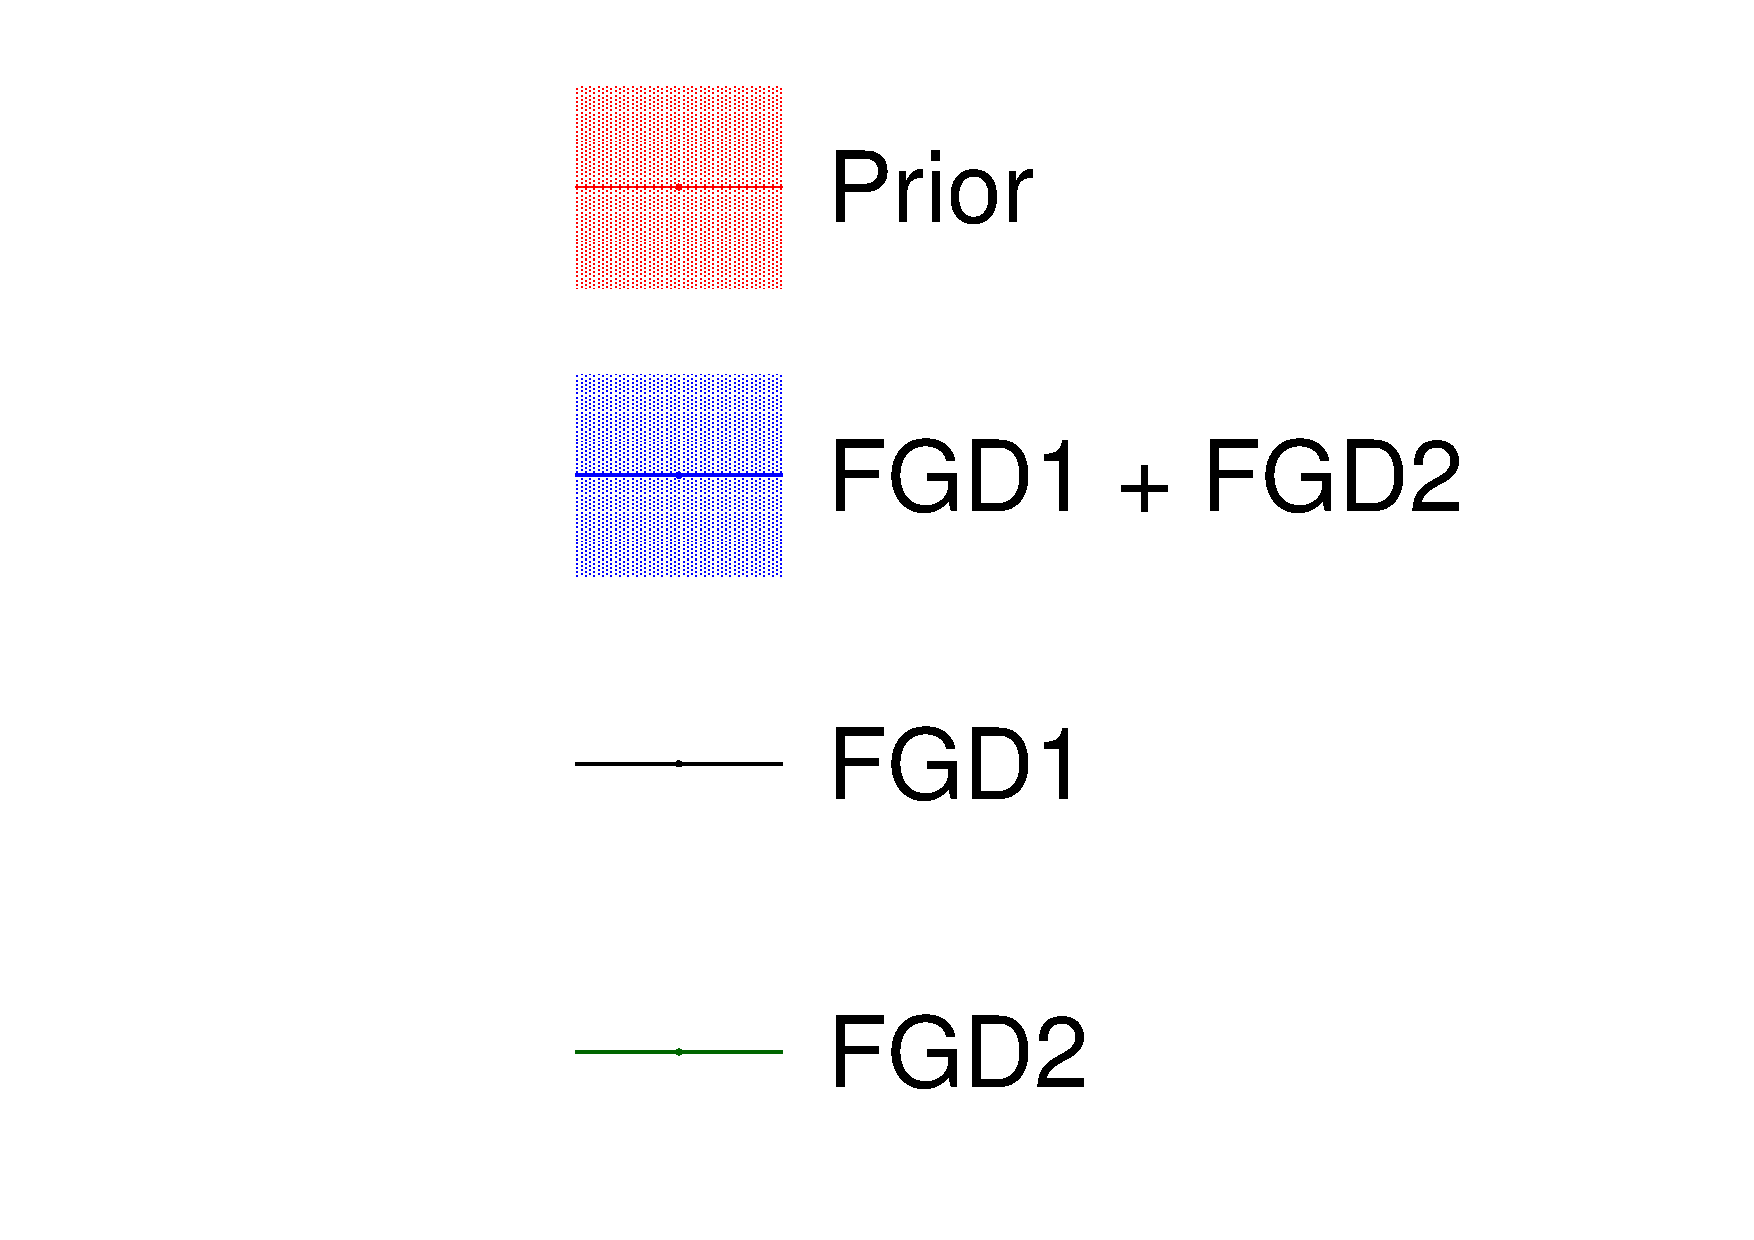
\includegraphics[width=1.0\linewidth, trim={5mm  90mm 0mm 0mm}, clip]{figs/fgdfits_leg}
\end{subfigure}
\begin{subfigure}{0.3\textwidth}
  \centering
  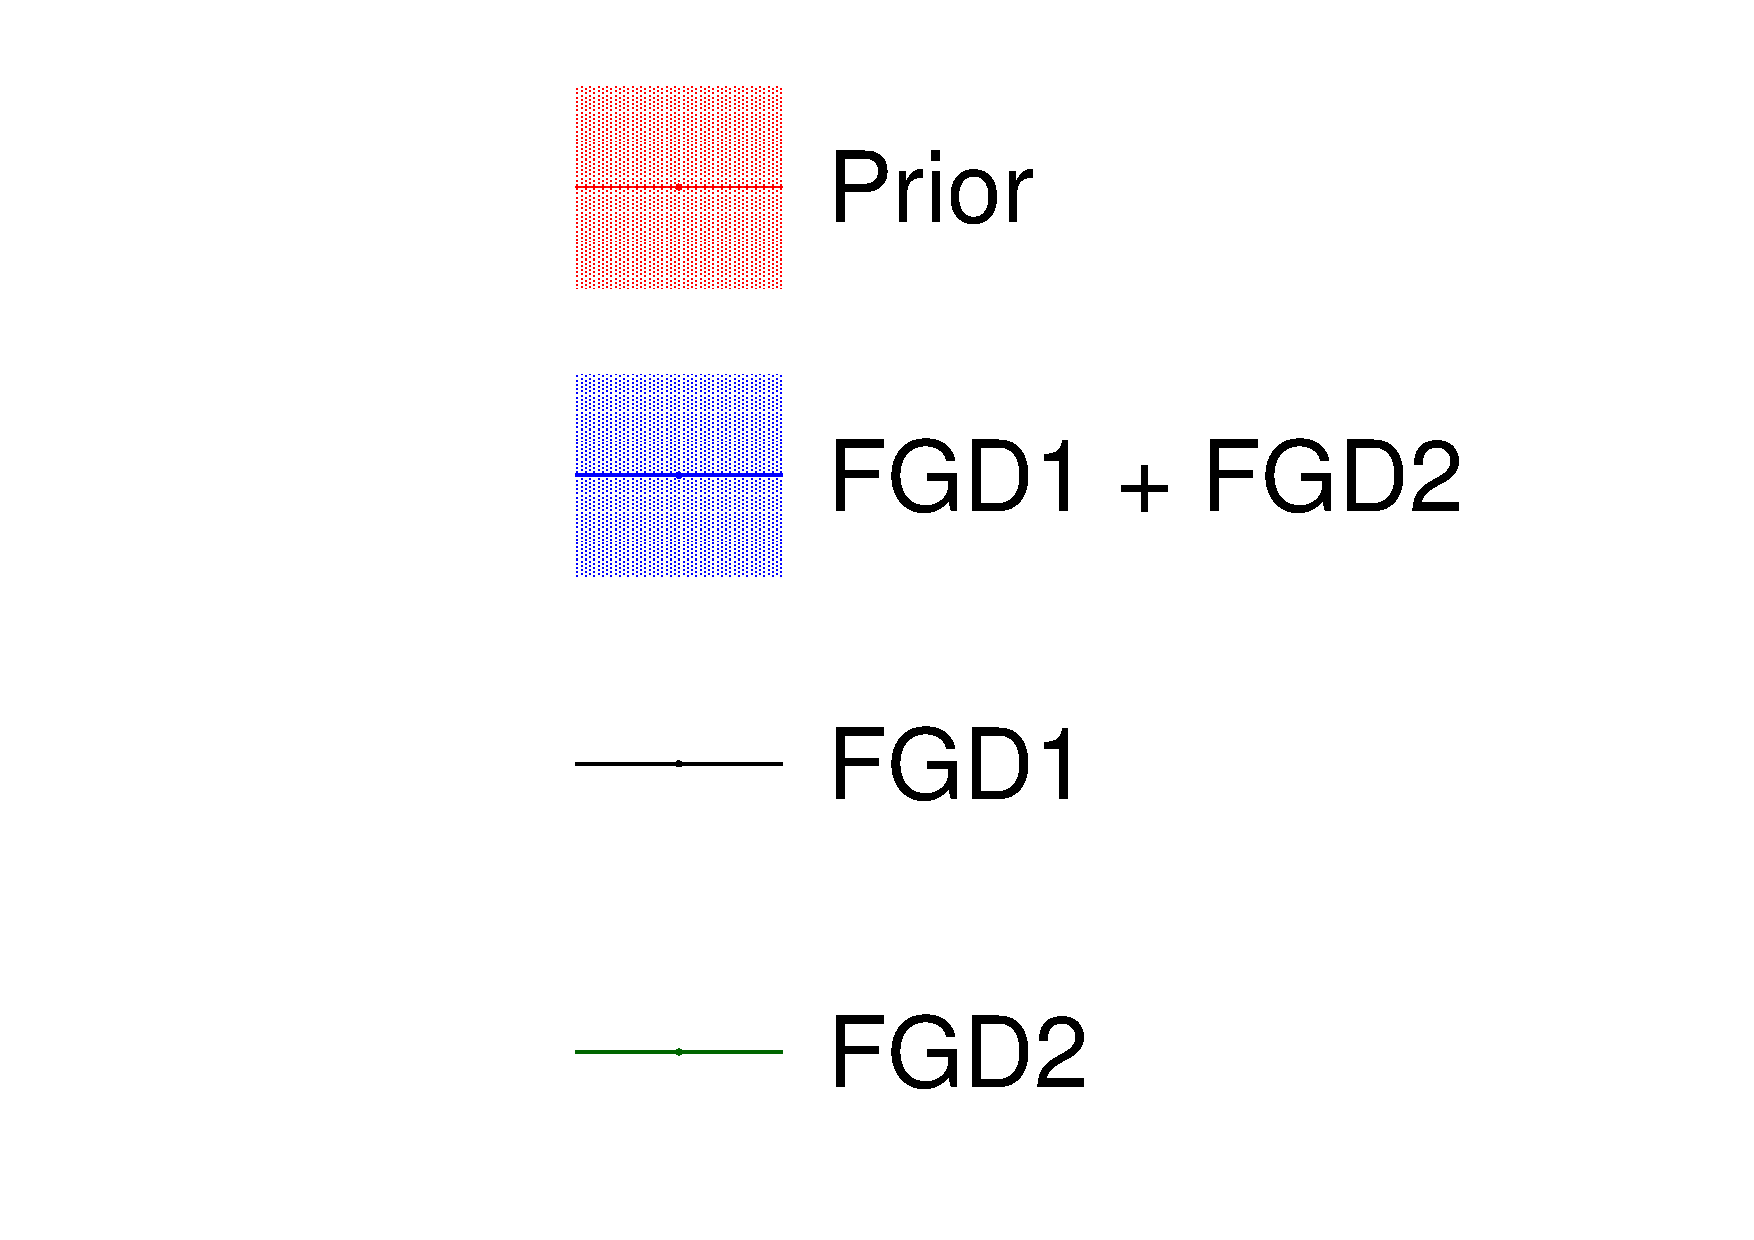
\includegraphics[width=1.0\linewidth, trim={5mm  0mm 0mm 95mm}, clip]{figs/fgdfits_leg}
\end{subfigure}
\begin{subfigure}{0.45\textwidth}
  \centering
  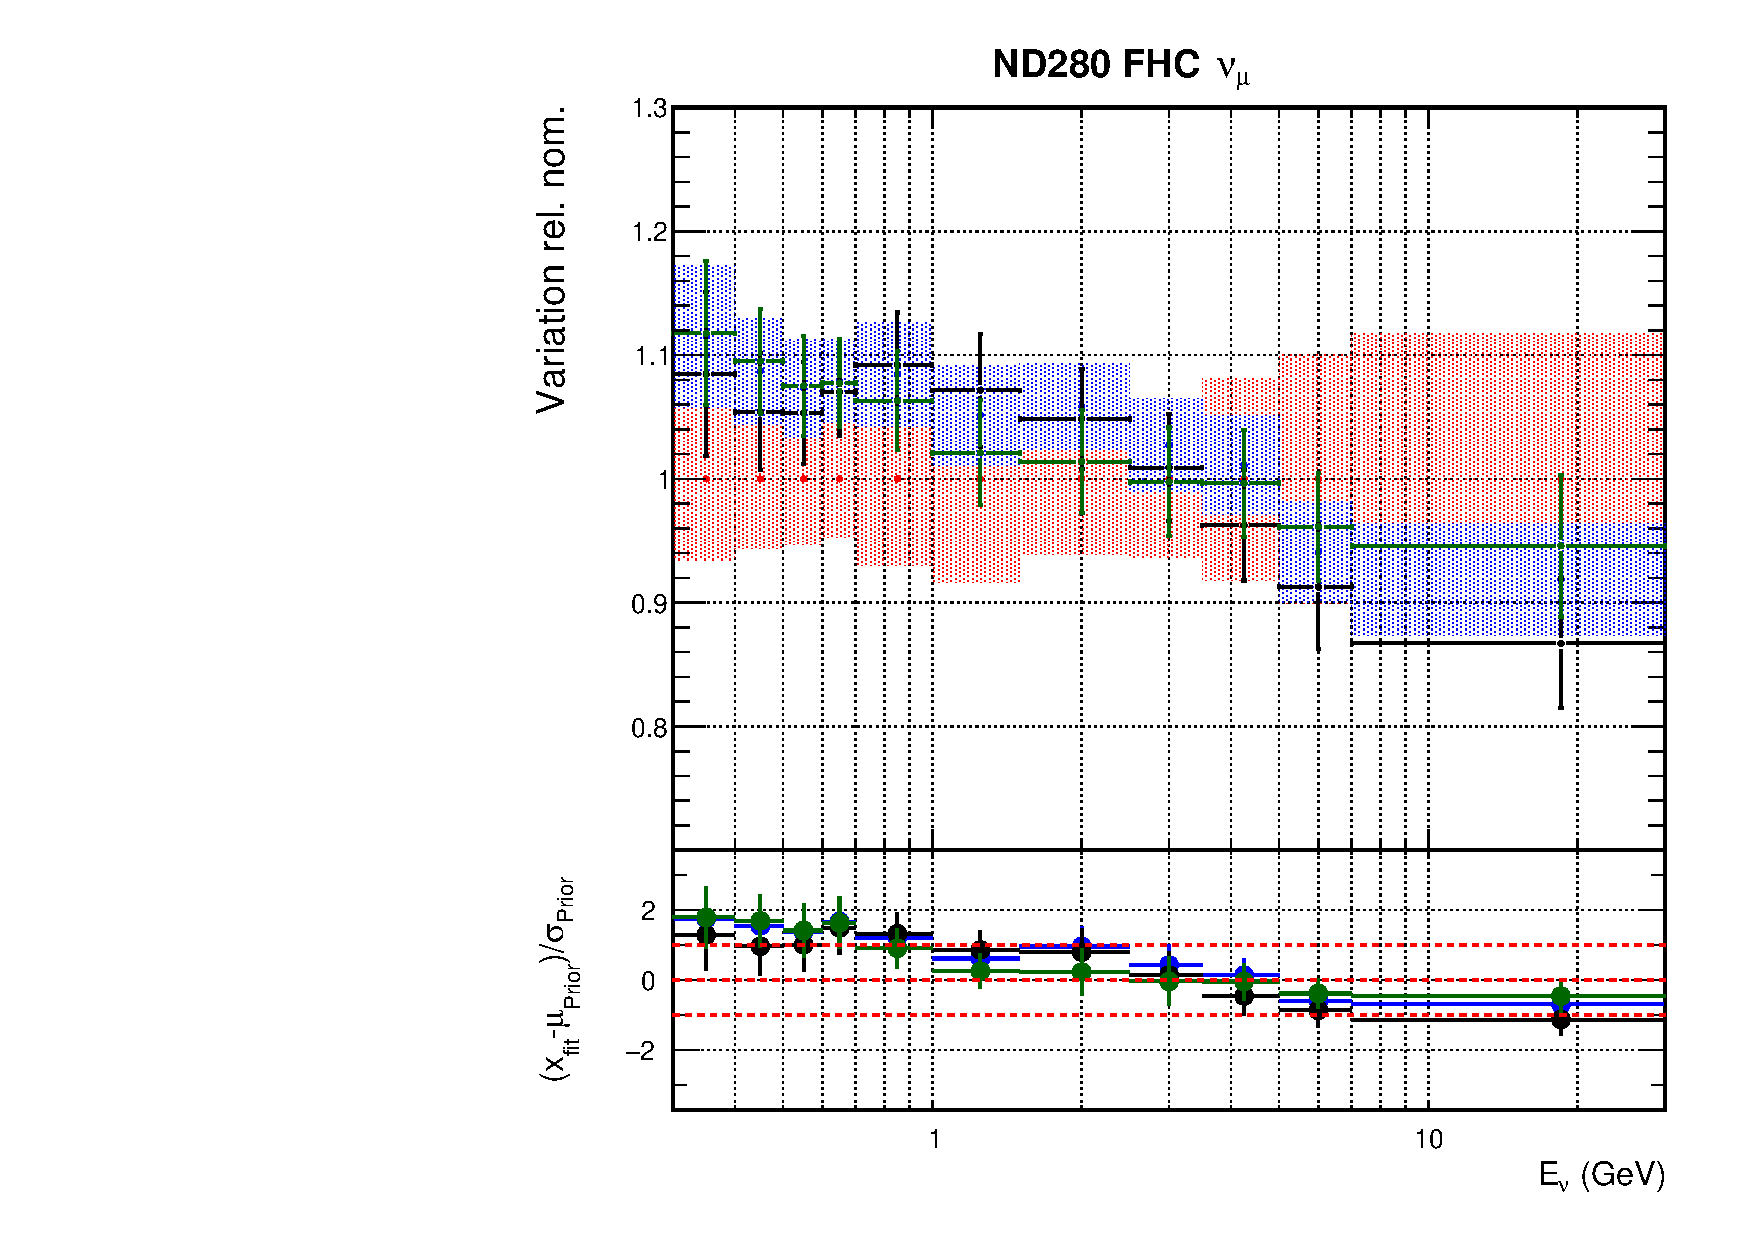
\includegraphics[width=0.75\linewidth]{figs/fgdfitsflux_0}
  \caption{ND FHC $\nu_{\mu}$}  
\end{subfigure}
\begin{subfigure}{0.45\textwidth}
  \centering
  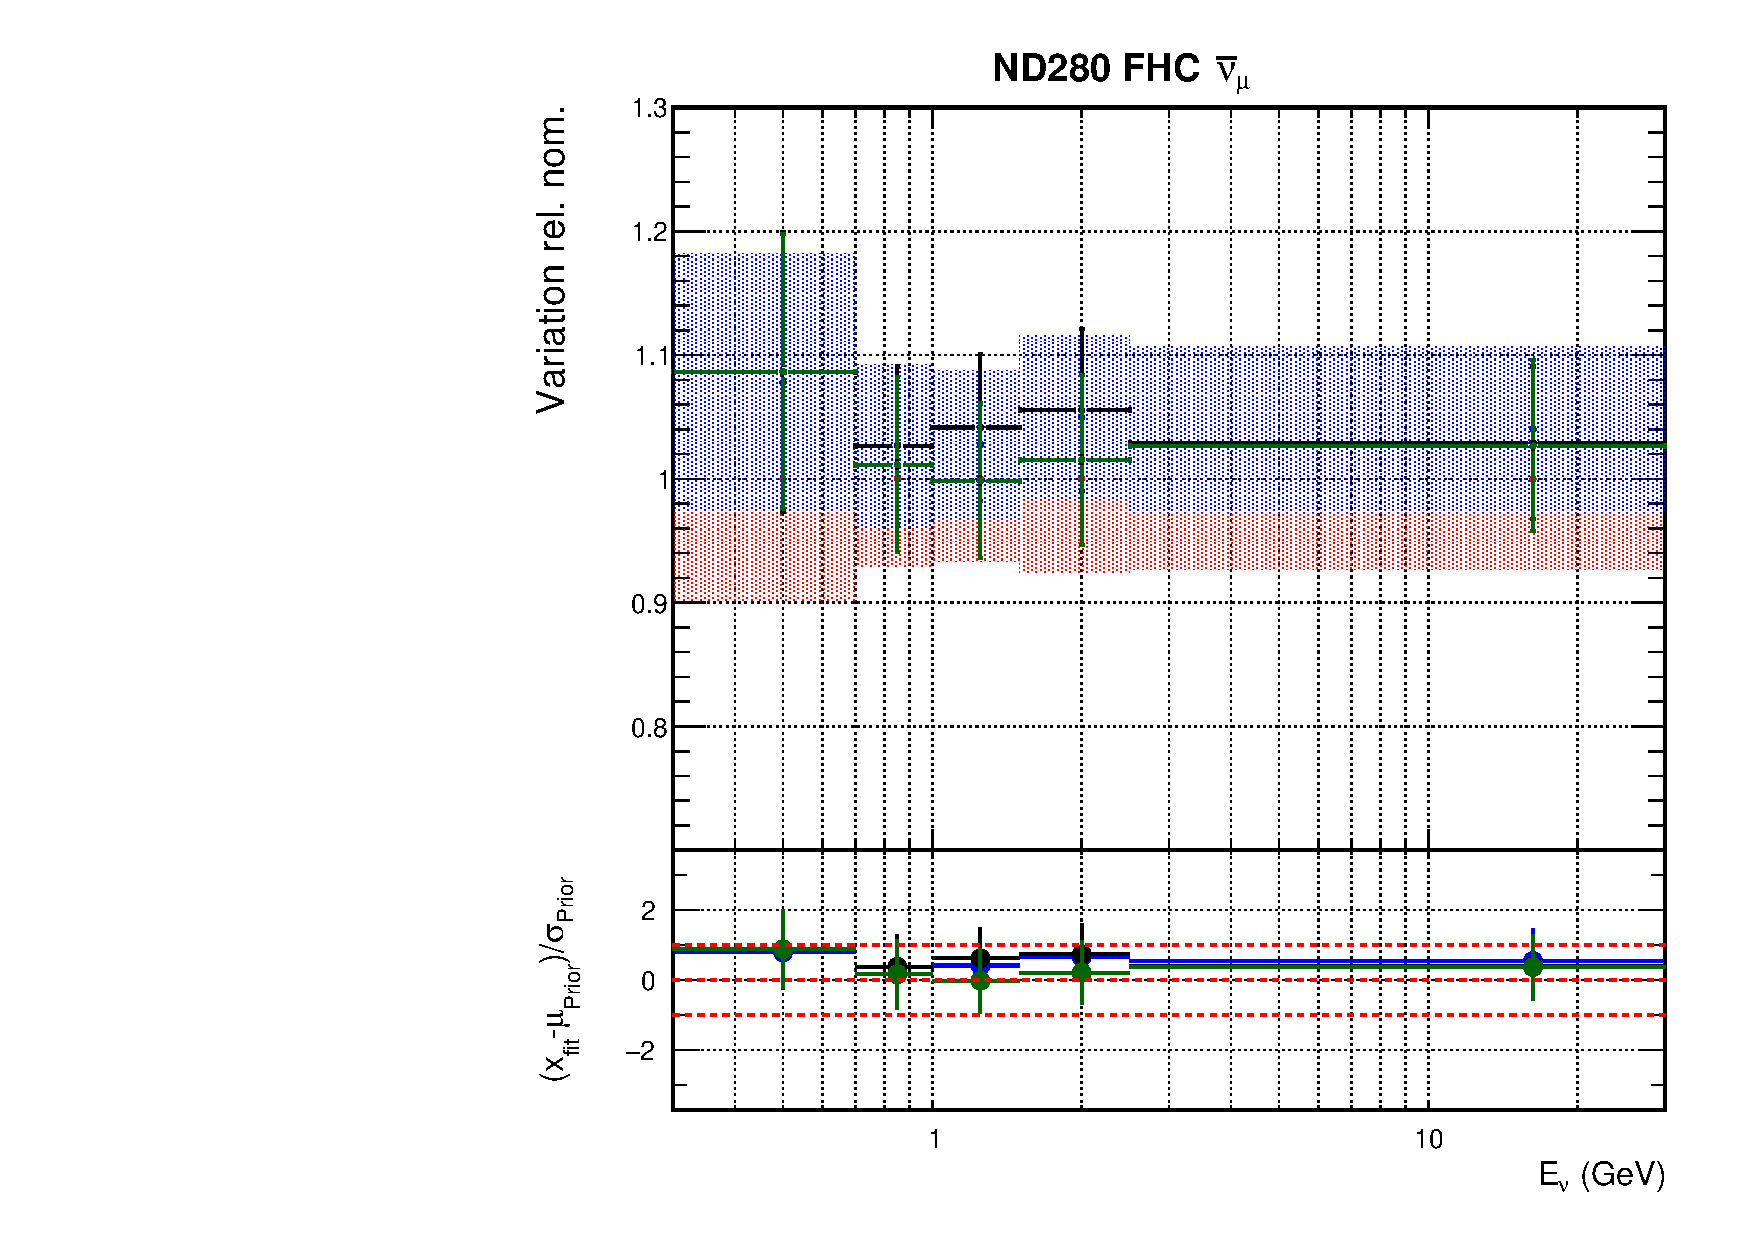
\includegraphics[width=0.75\linewidth]{figs/fgdfitsflux_1}
  \caption{ND FHC $\bar{\nu_{\mu}}$}
\end{subfigure}
\begin{subfigure}{0.45\textwidth}
  \centering
  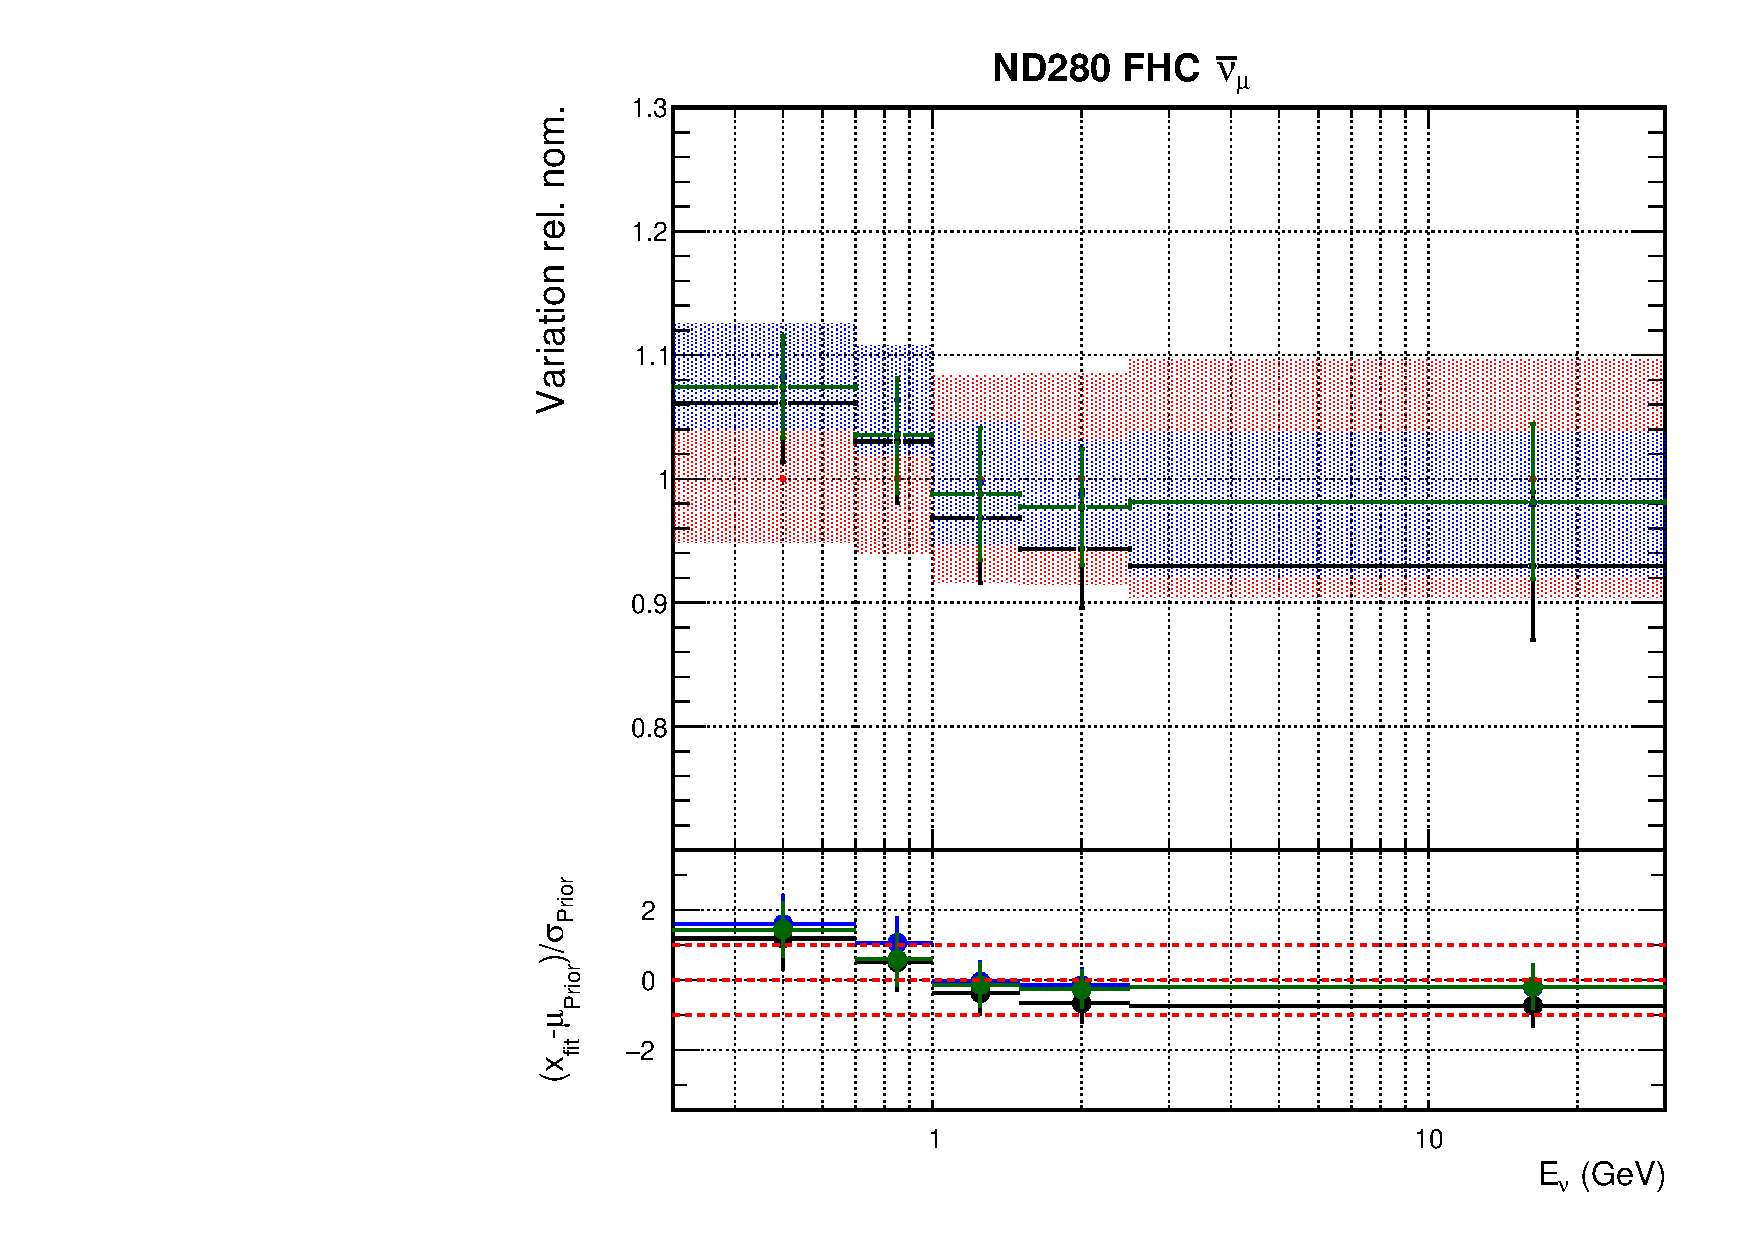
\includegraphics[width=0.75\linewidth]{figs/fgdfitsflux_2}
  \caption{ND FHC $\nu_e$}
\end{subfigure}
\begin{subfigure}{0.45\textwidth}
  \centering
  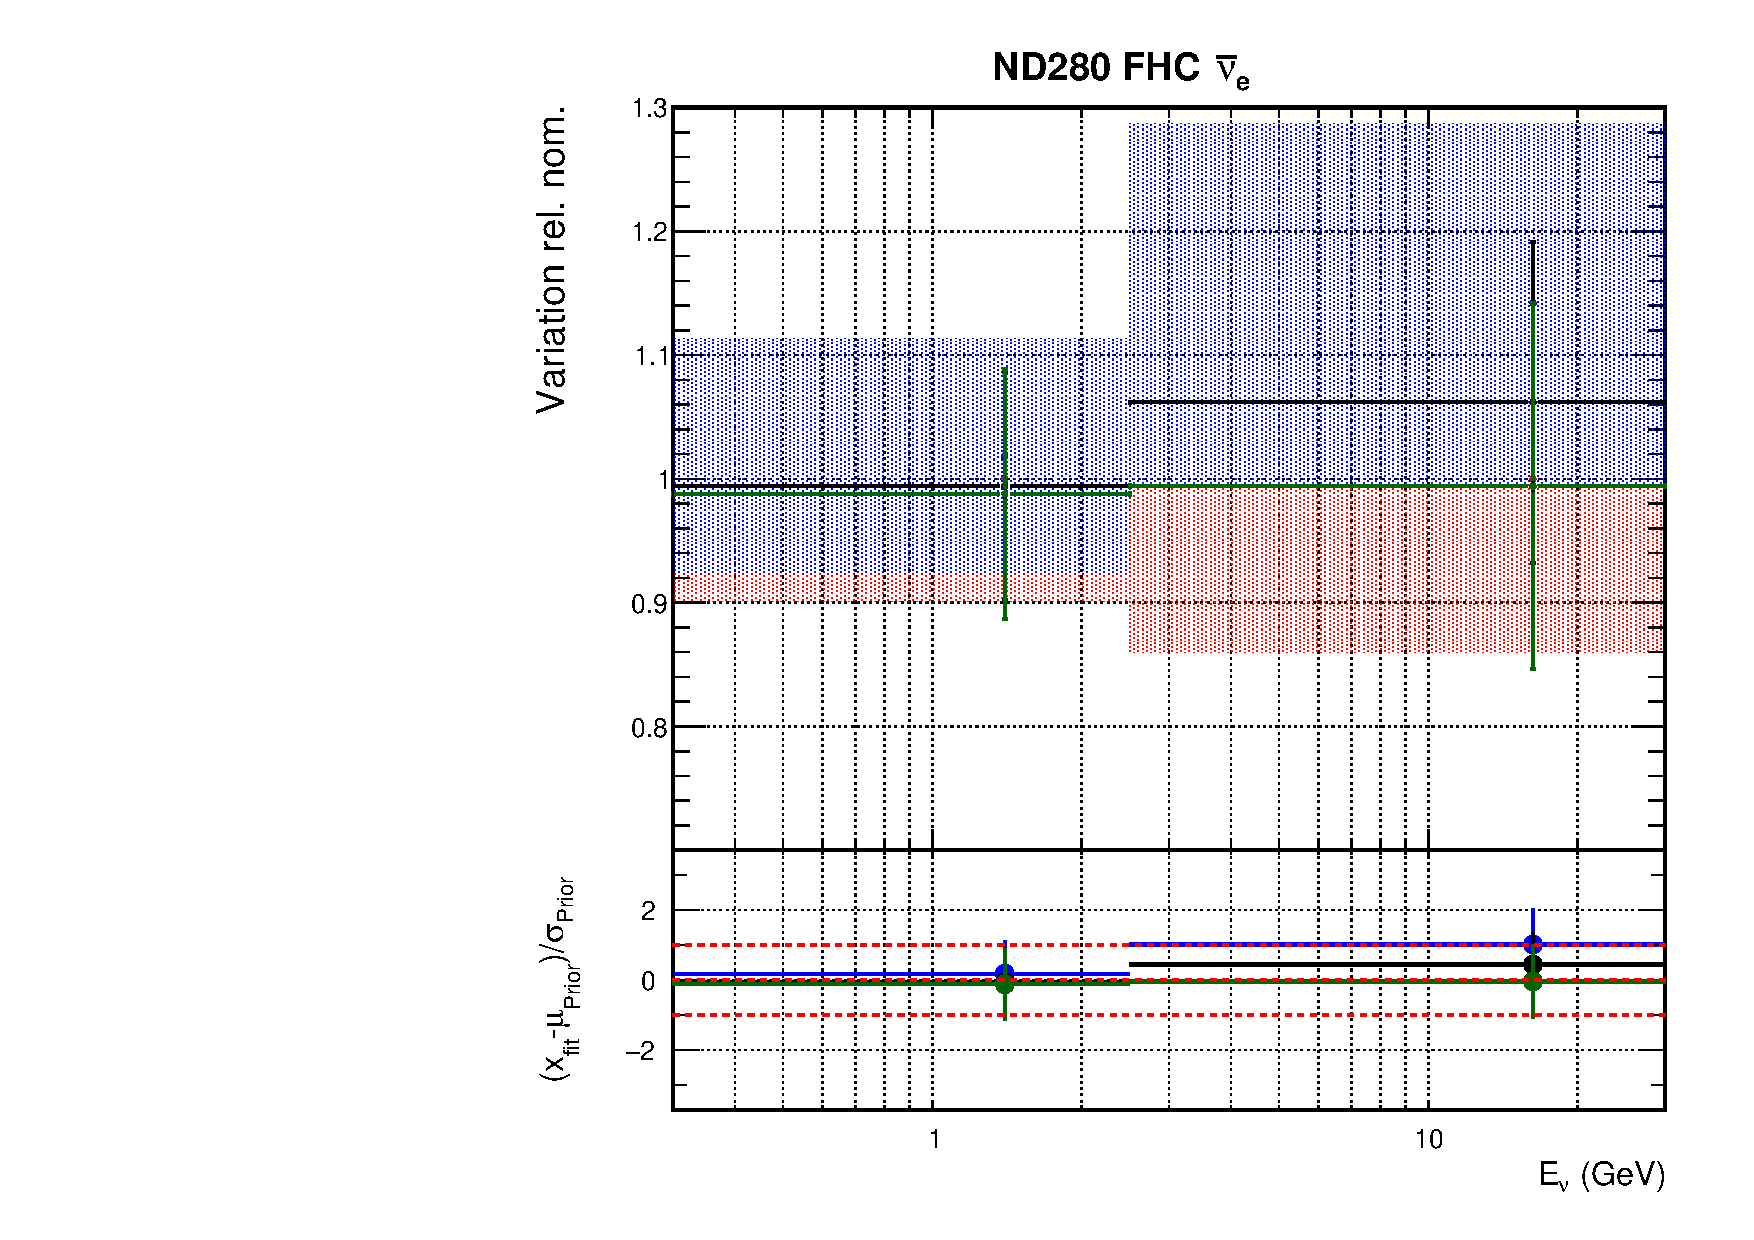
\includegraphics[width=0.75\linewidth]{figs/fgdfitsflux_3}
  \caption{ND FHC $\bar{\nu_{e}}$}  
\end{subfigure}
\begin{subfigure}{0.45\textwidth}
  \centering
  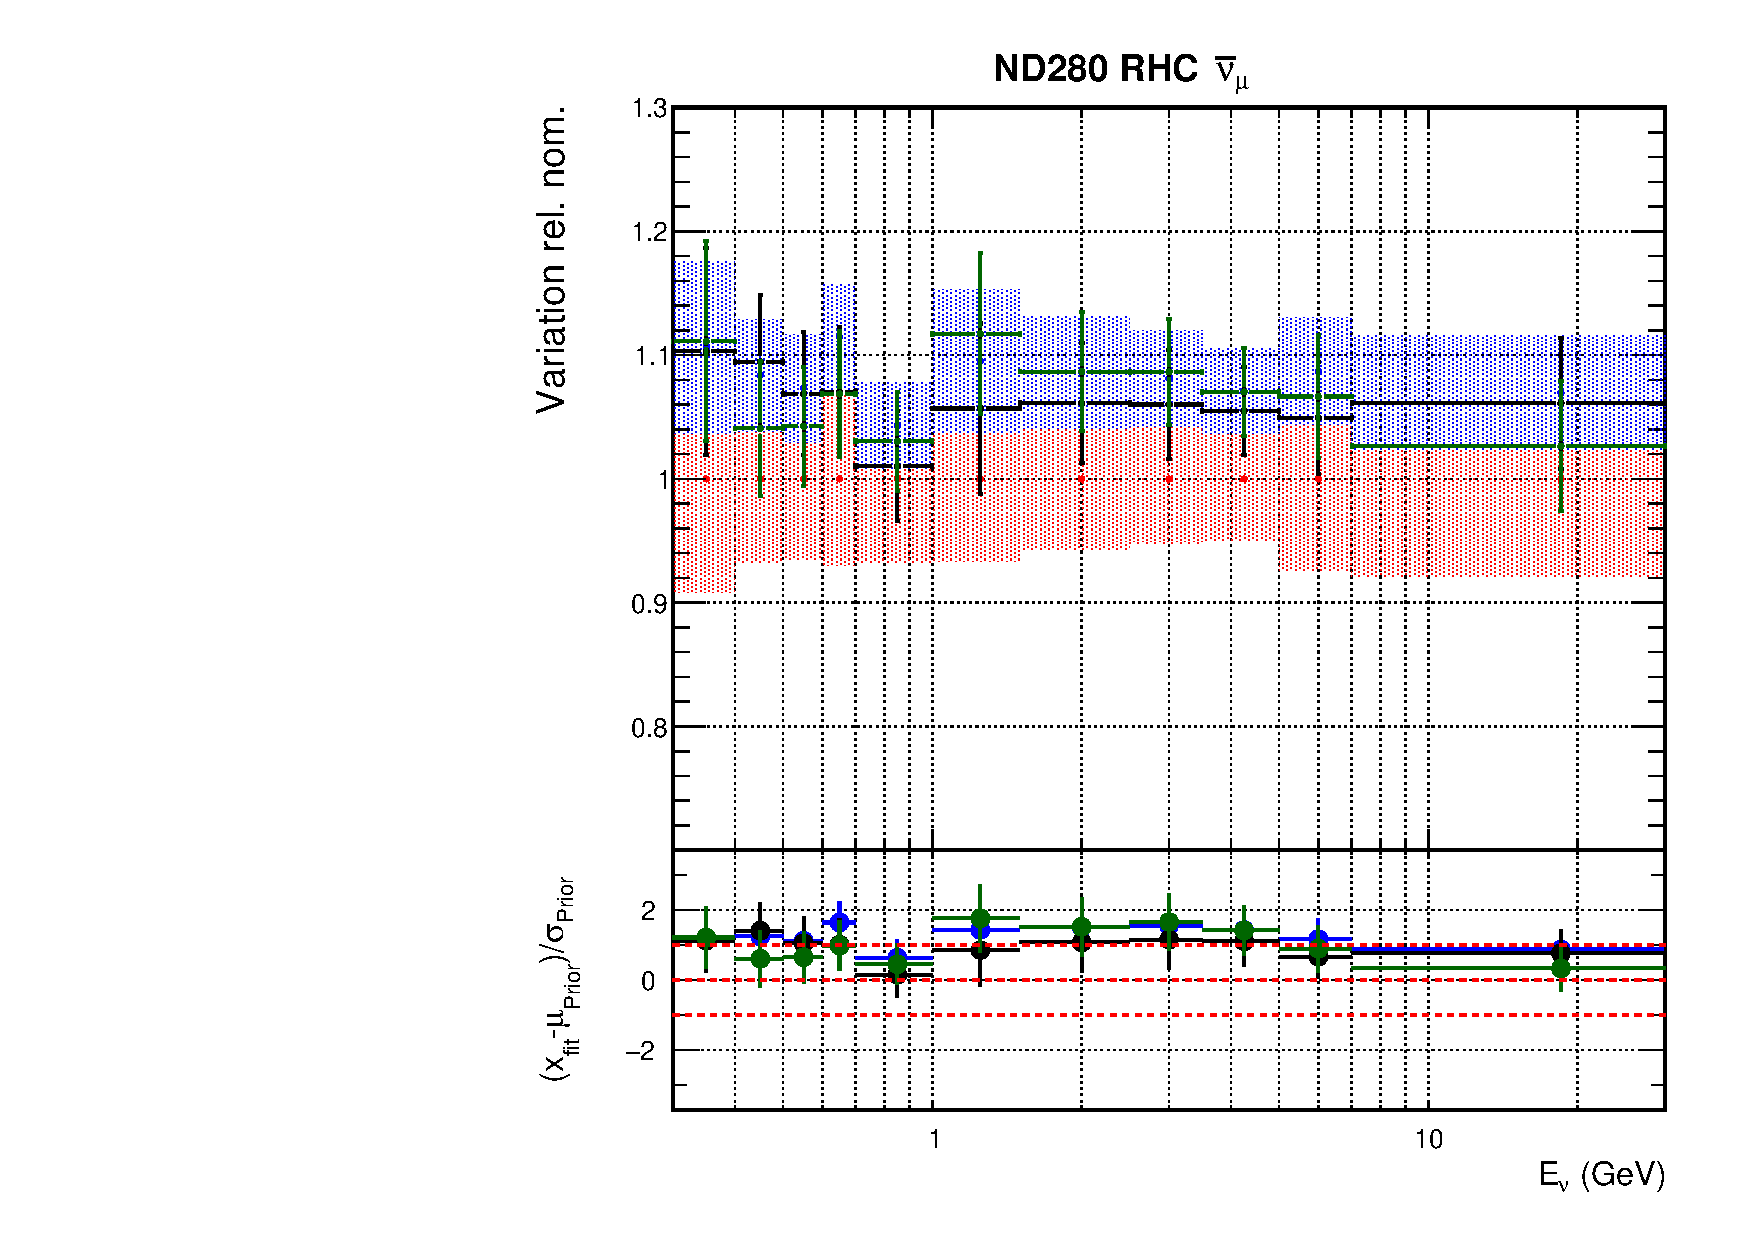
\includegraphics[width=0.75\linewidth]{figs/fgdfitsflux_4}
  \caption{ND RHC $\nu_{\mu}$}
\end{subfigure}
\begin{subfigure}{0.45\textwidth}
  \centering
  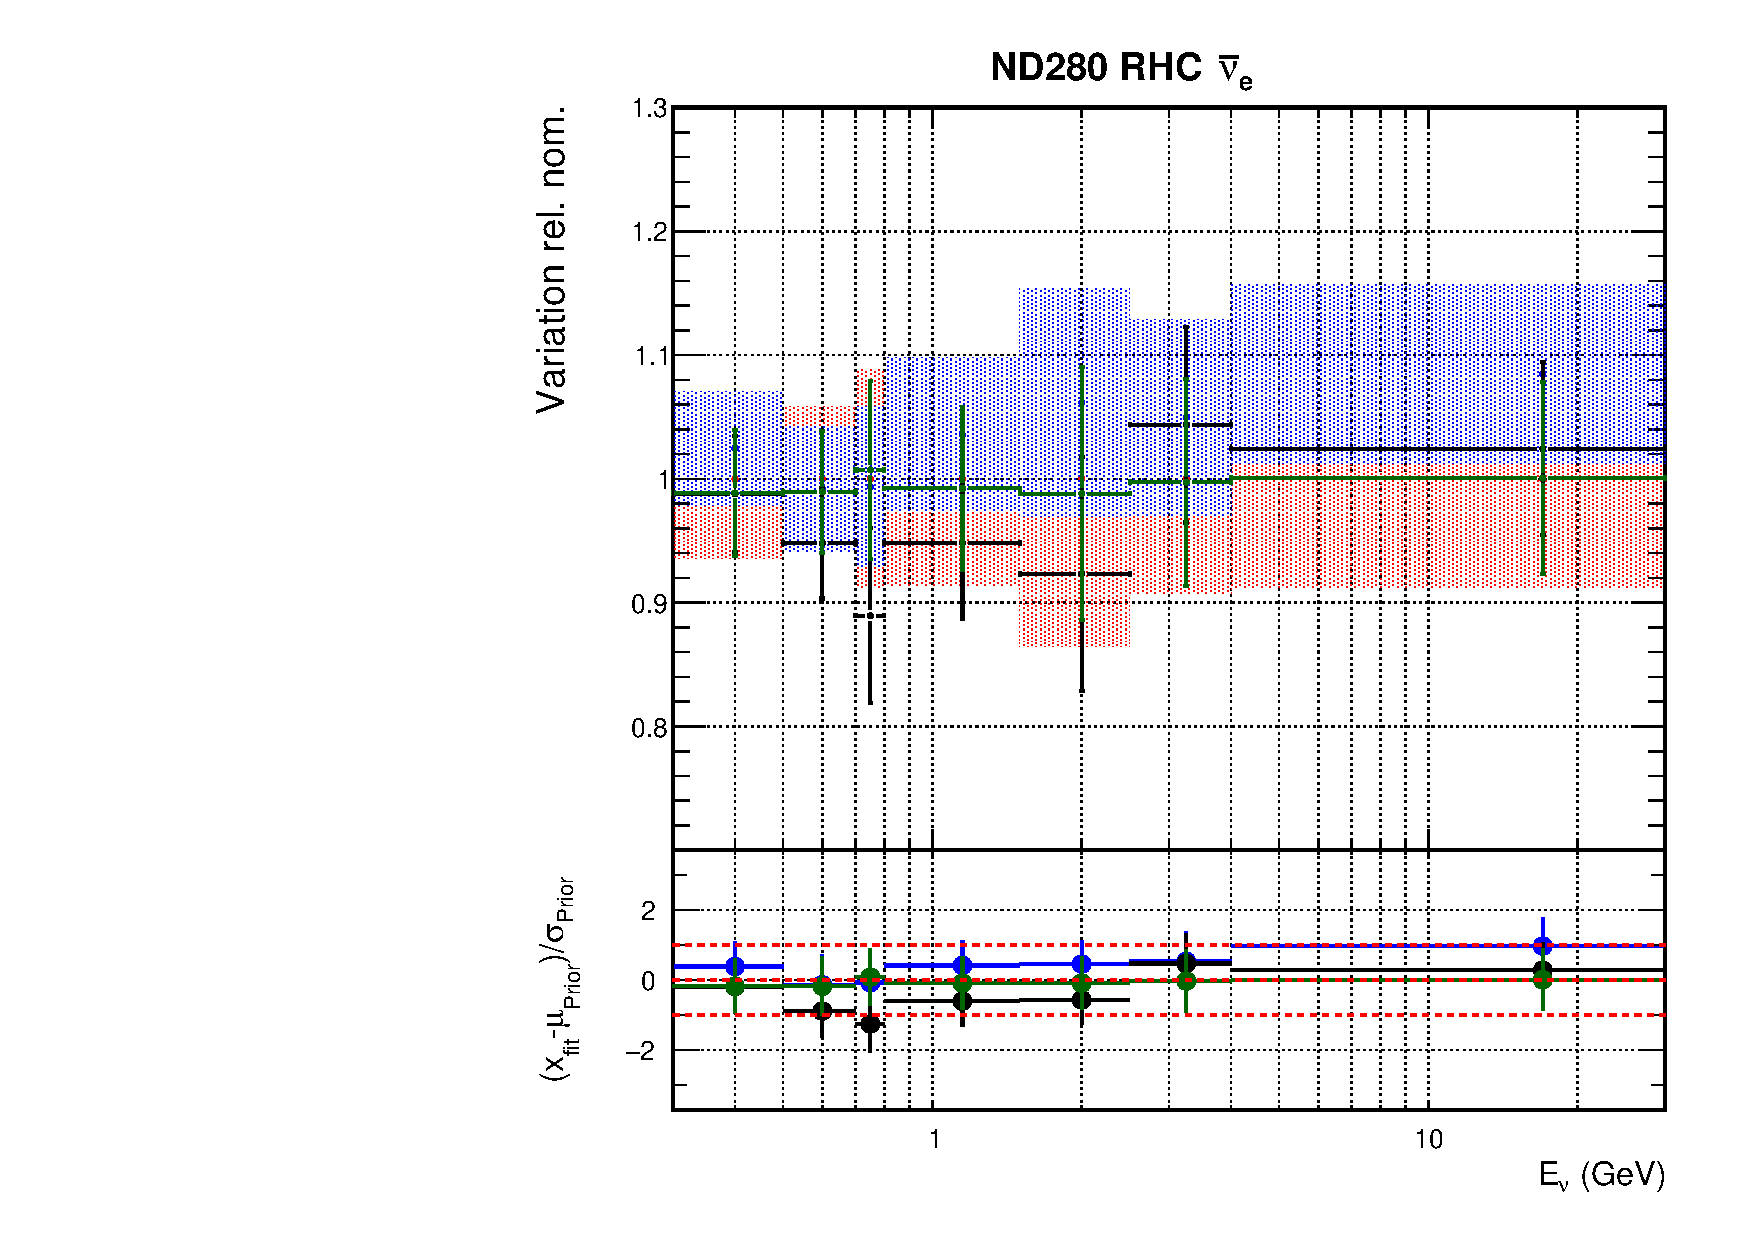
\includegraphics[width=0.75\linewidth]{figs/fgdfitsflux_5}
  \caption{ND RHC $\bar{\nu_{\mu}}$}
\end{subfigure}
\begin{subfigure}{0.45\textwidth}
  \centering
  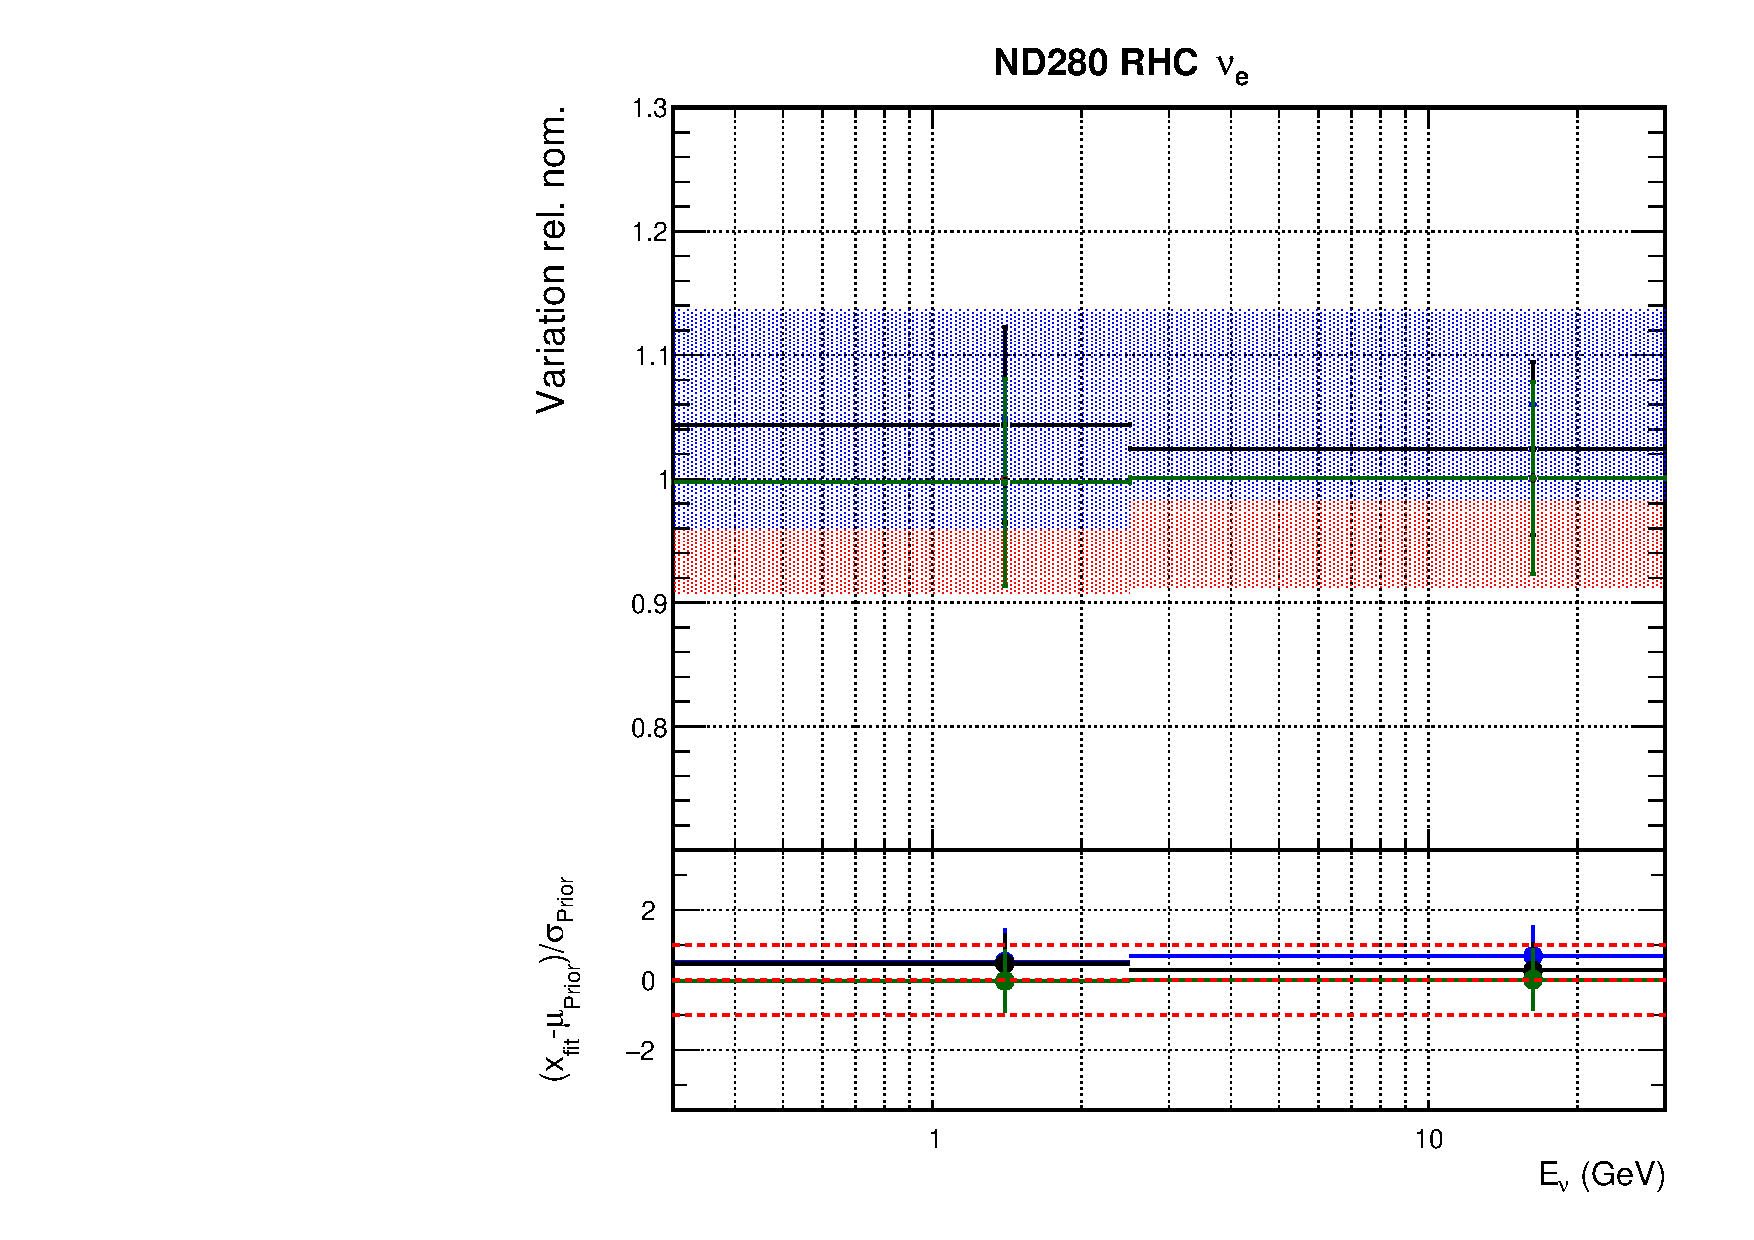
\includegraphics[width=0.75\linewidth]{figs/fgdfitsflux_6}
  \caption{ND RHC $\nu_{e}$}
\end{subfigure}
\begin{subfigure}{0.45\textwidth}
  \centering
  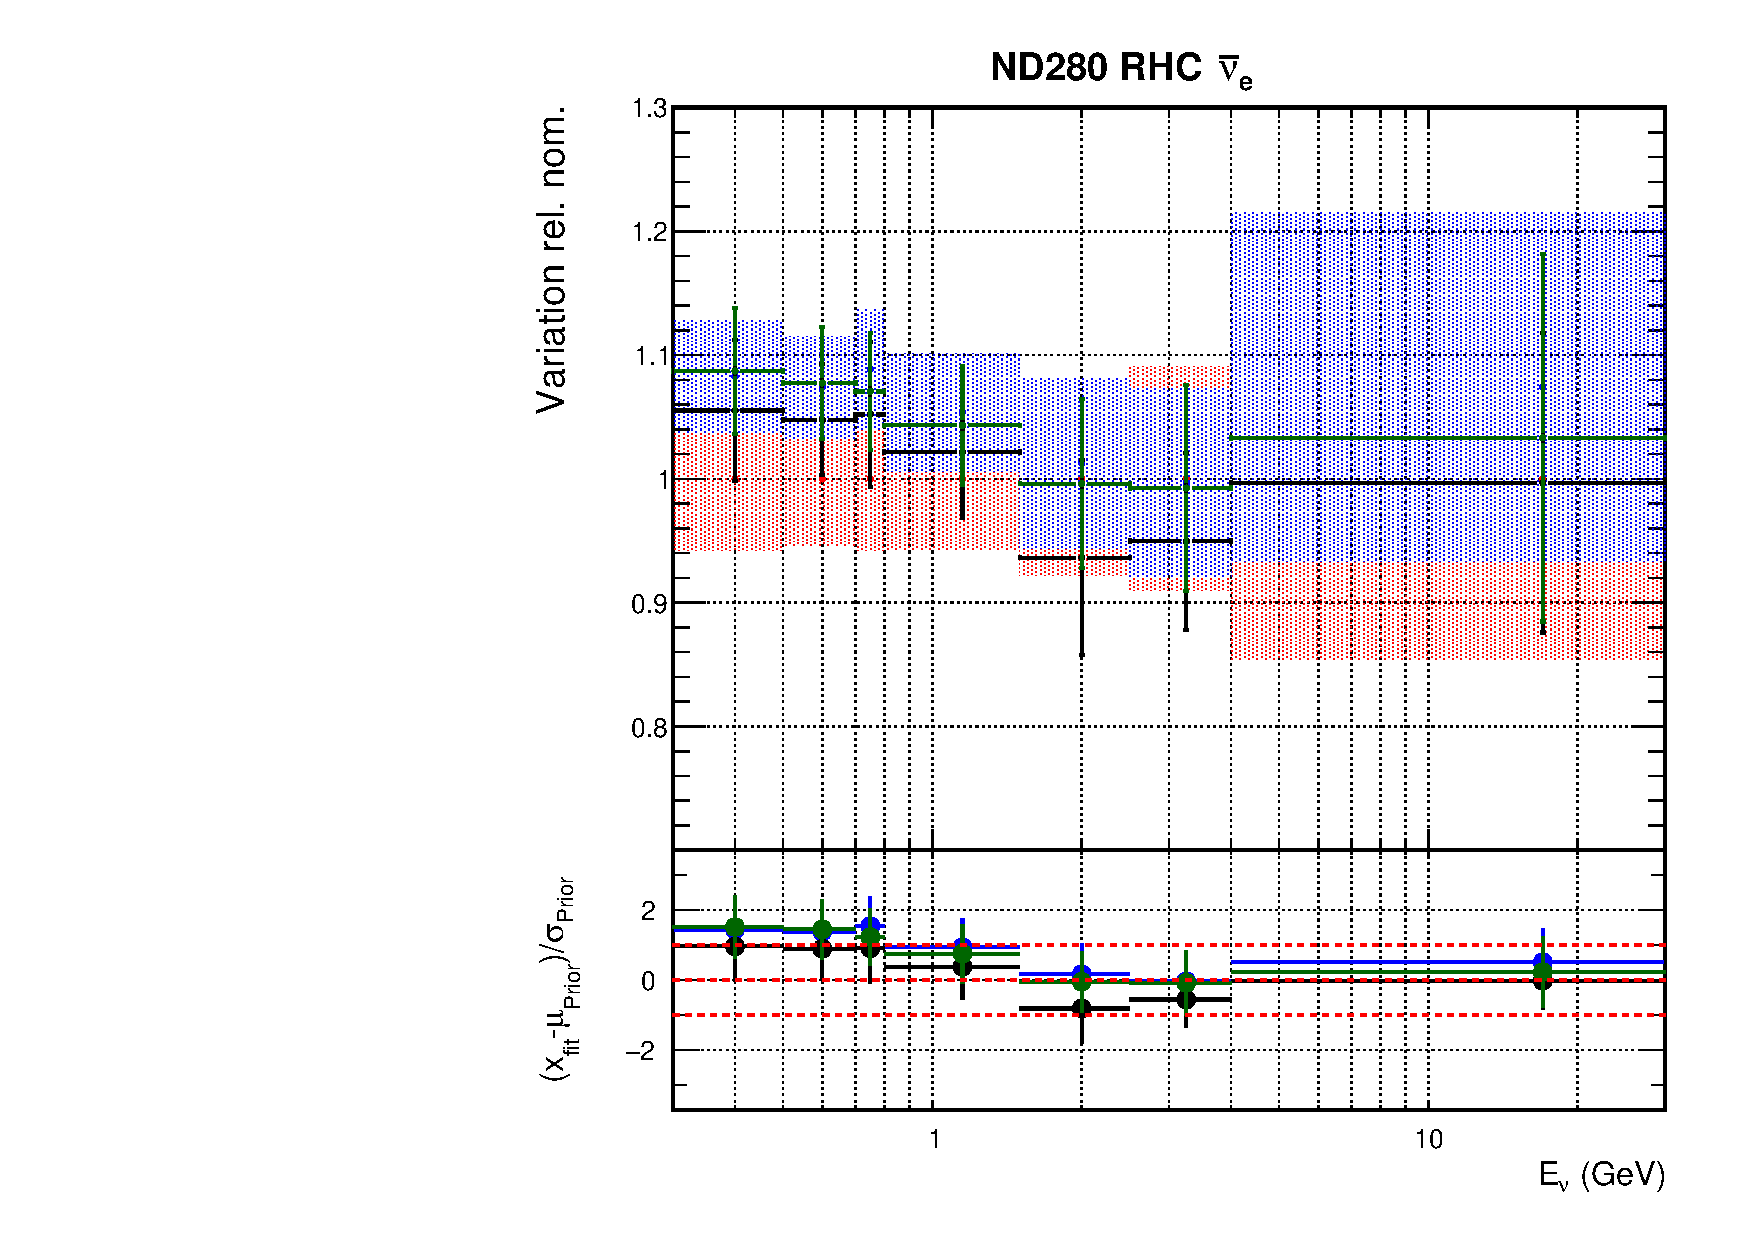
\includegraphics[width=0.75\linewidth]{figs/fgdfitsflux_7}
  \caption{ND RHC $\bar{\nu_e}$}
\end{subfigure}
\caption{ND280 flux parameters for the FGD1 and 2 only fits.}
\label{fig:fgdfluxND}
\end{figure}

\begin{figure}
\centering
\begin{subfigure}{0.3\textwidth}
  \centering
  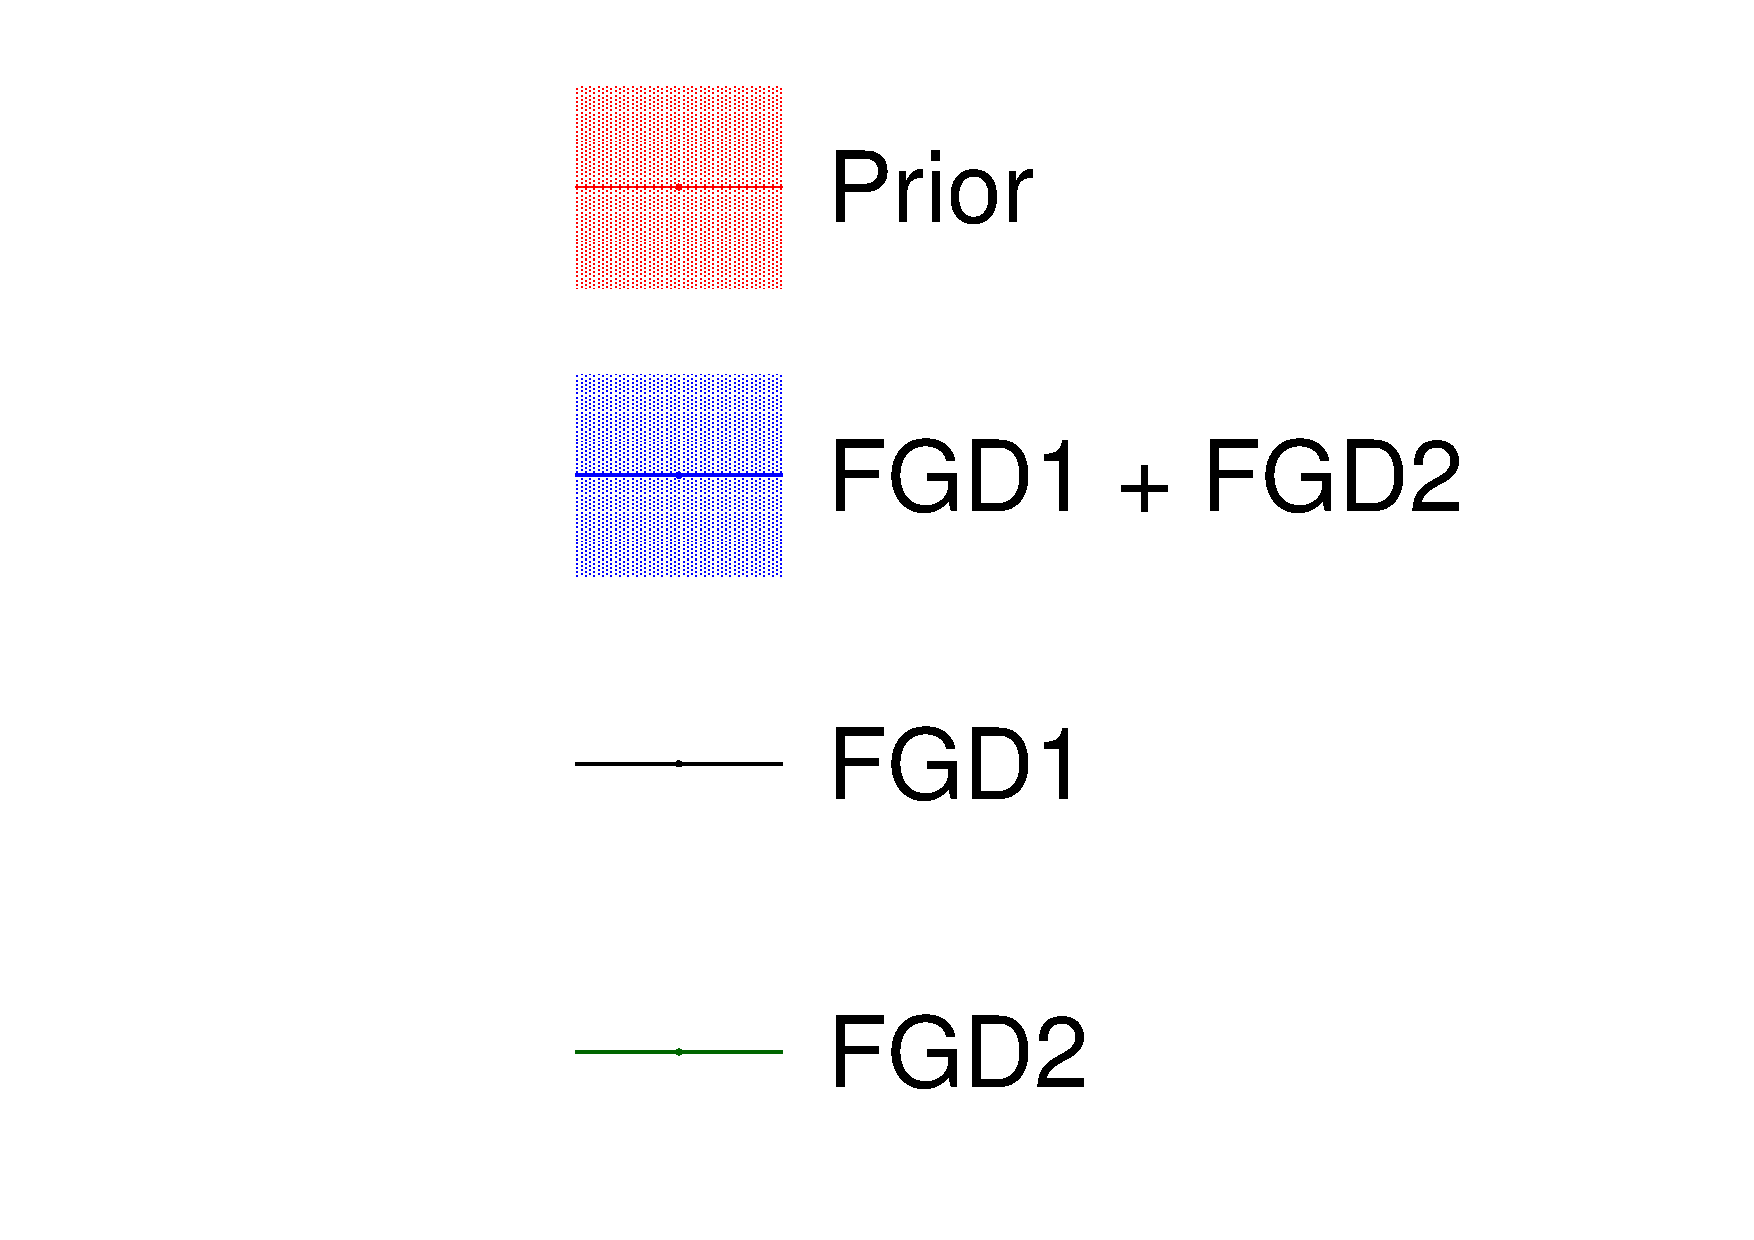
\includegraphics[width=1.0\linewidth, trim={5mm  90mm 0mm 0mm}, clip]{figs/fgdfits_leg}
\end{subfigure}
\begin{subfigure}{0.3\textwidth}
  \centering
  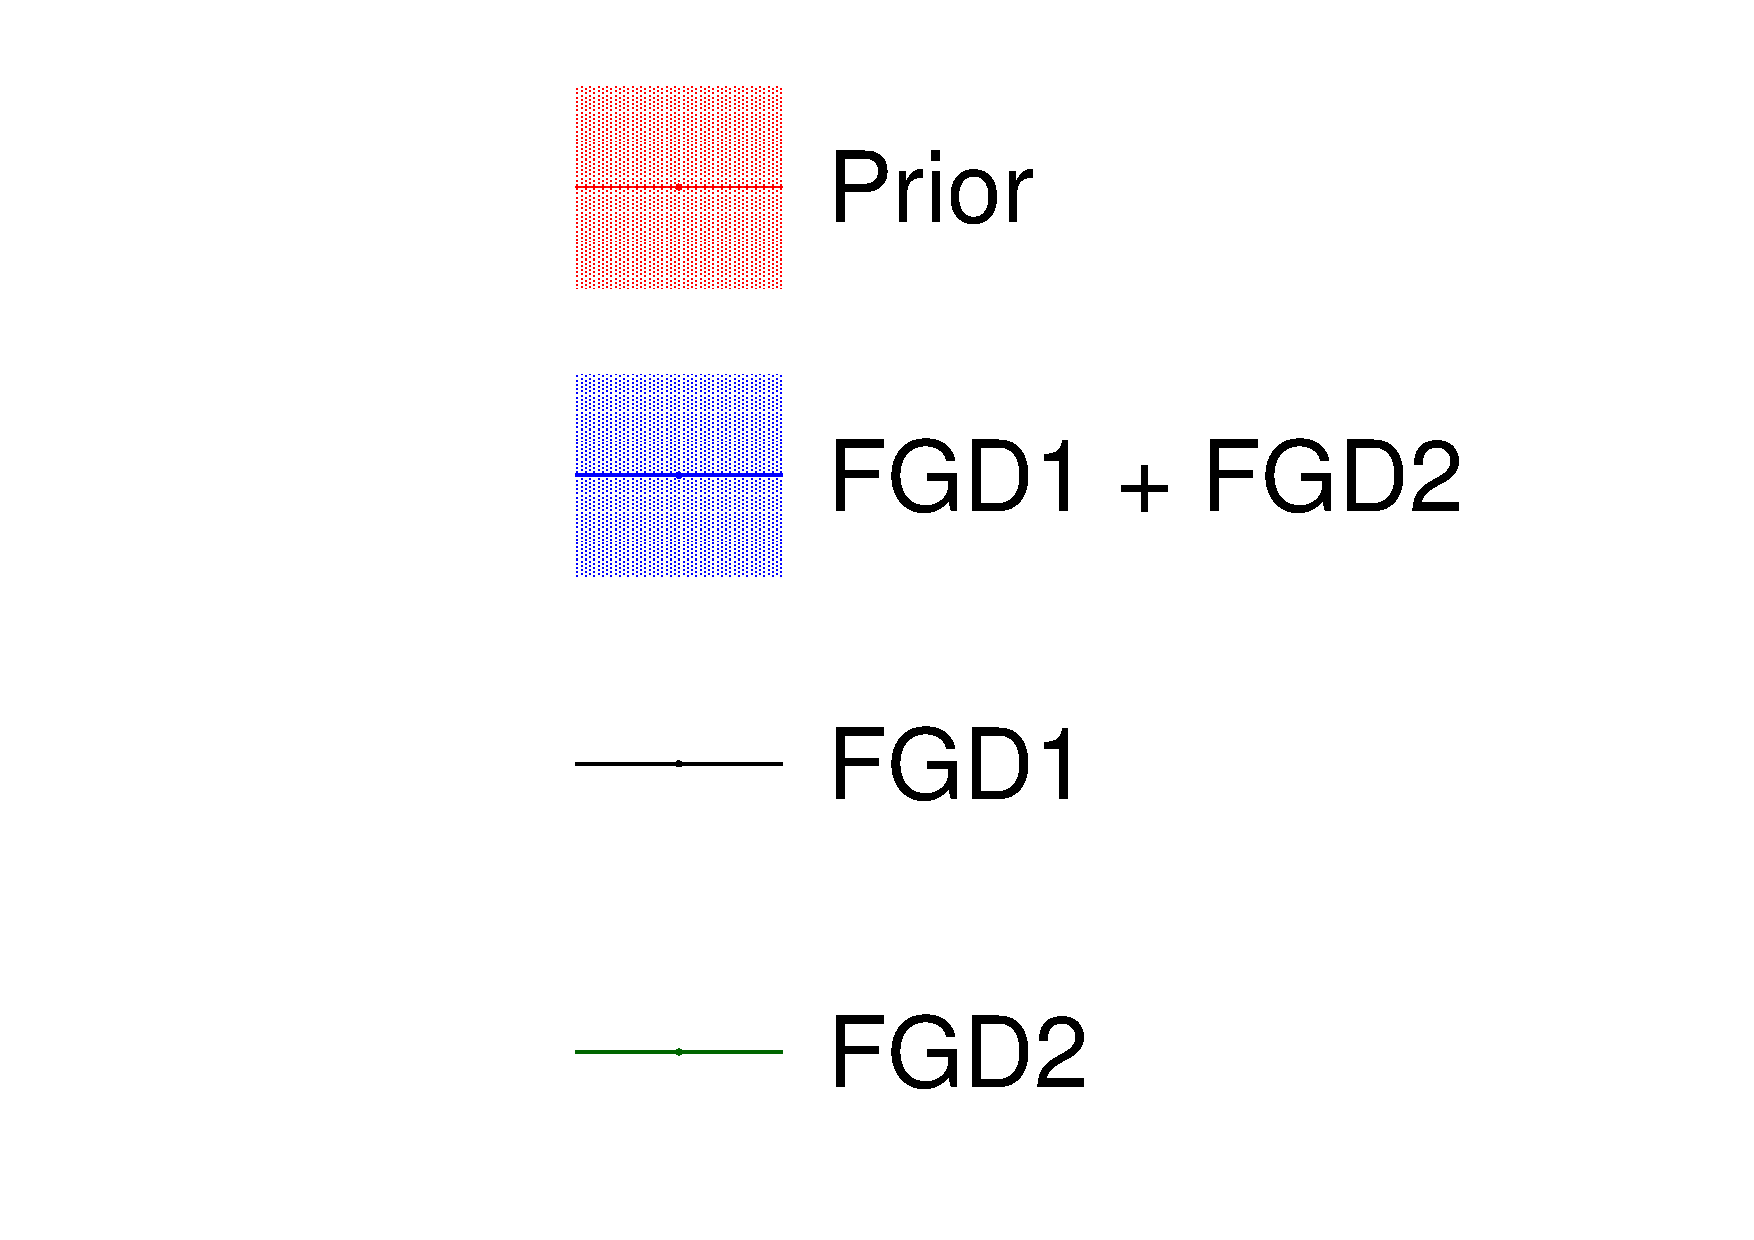
\includegraphics[width=1.0\linewidth, trim={5mm  0mm 0mm 95mm}, clip]{figs/fgdfits_leg}
\end{subfigure}
\begin{subfigure}{0.45\textwidth}
  \centering
  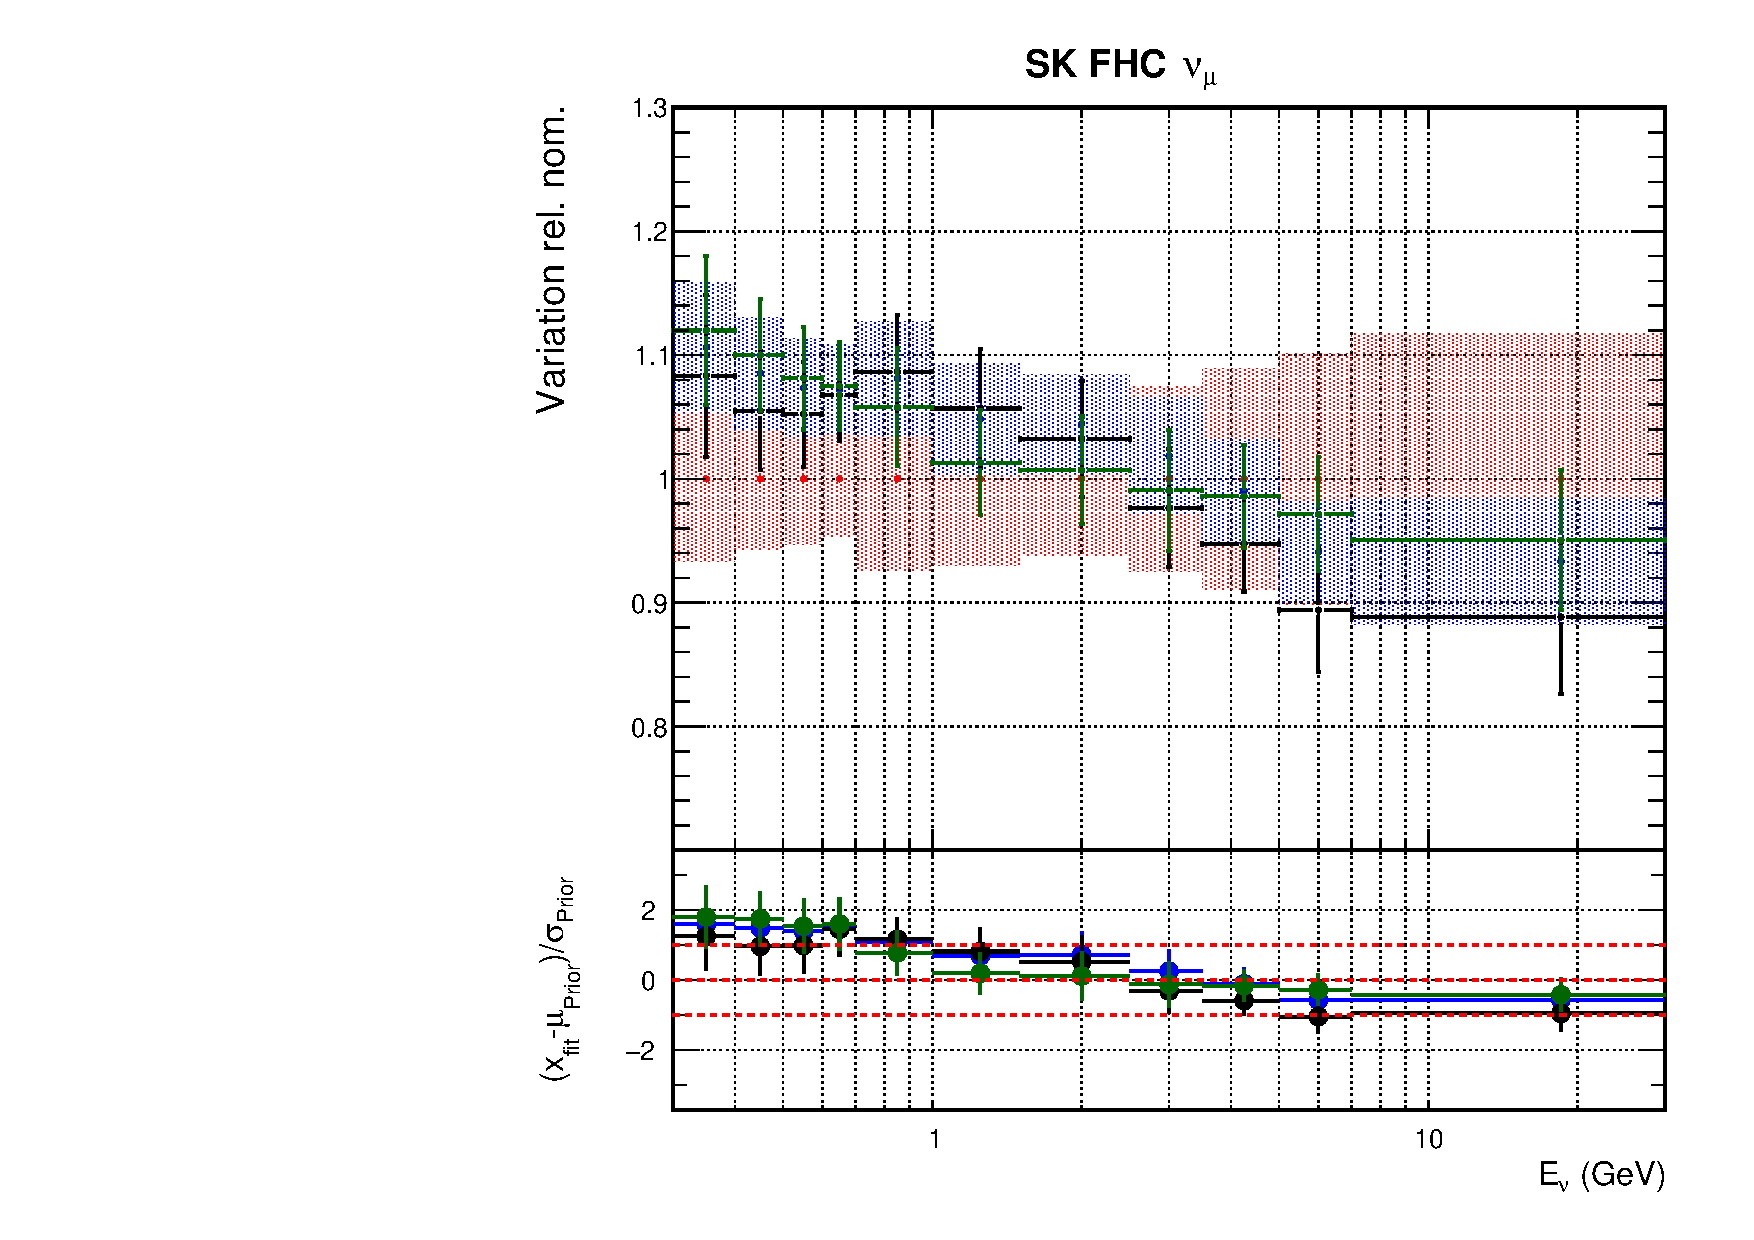
\includegraphics[width=0.75\linewidth]{figs/fgdfitsflux_8}
  \caption{\SK FHC $\nu_{\mu}$}
\end{subfigure}
\begin{subfigure}{0.45\textwidth}
  \centering
  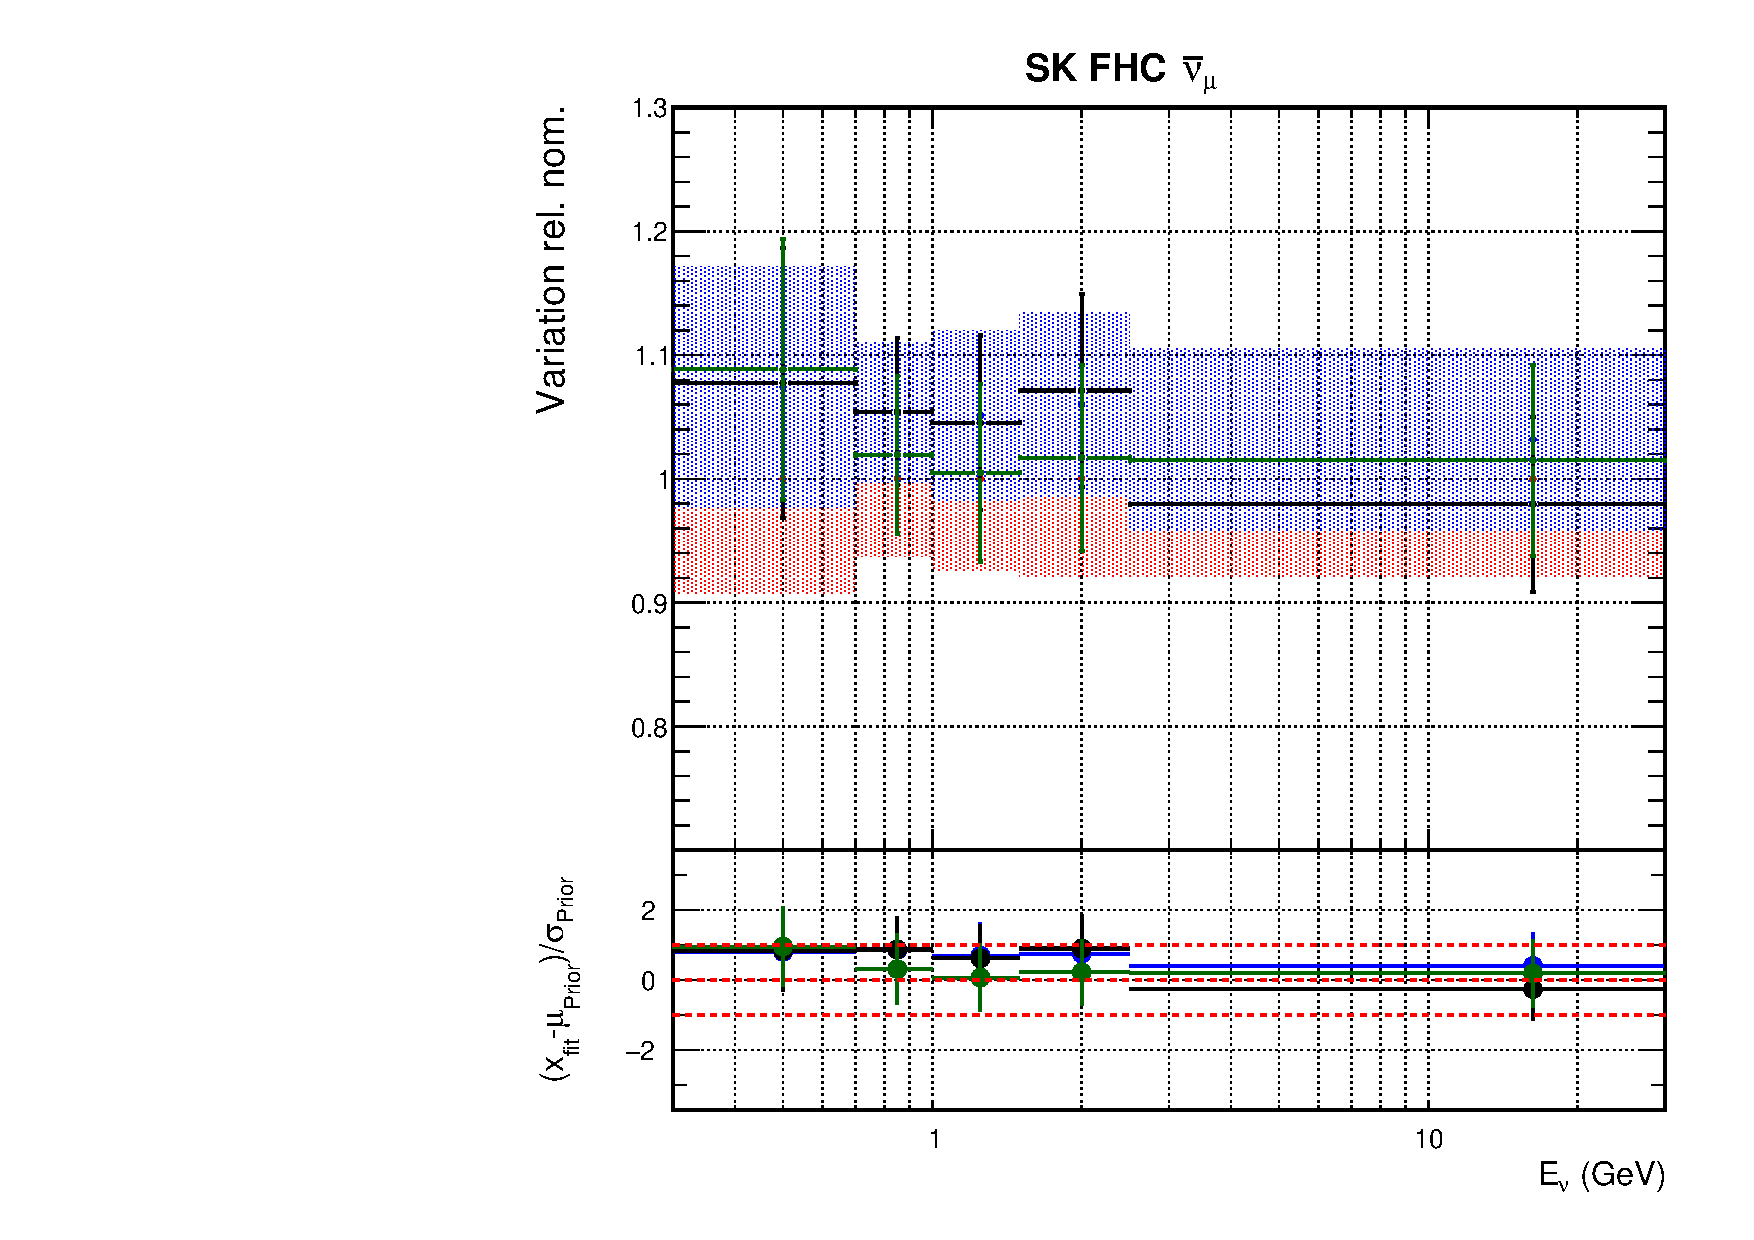
\includegraphics[width=0.75\linewidth]{figs/fgdfitsflux_9}
  \caption{\SK FHC $\bar{\nu_{\mu}}$}
\end{subfigure}
\begin{subfigure}{0.45\textwidth}
  \centering
  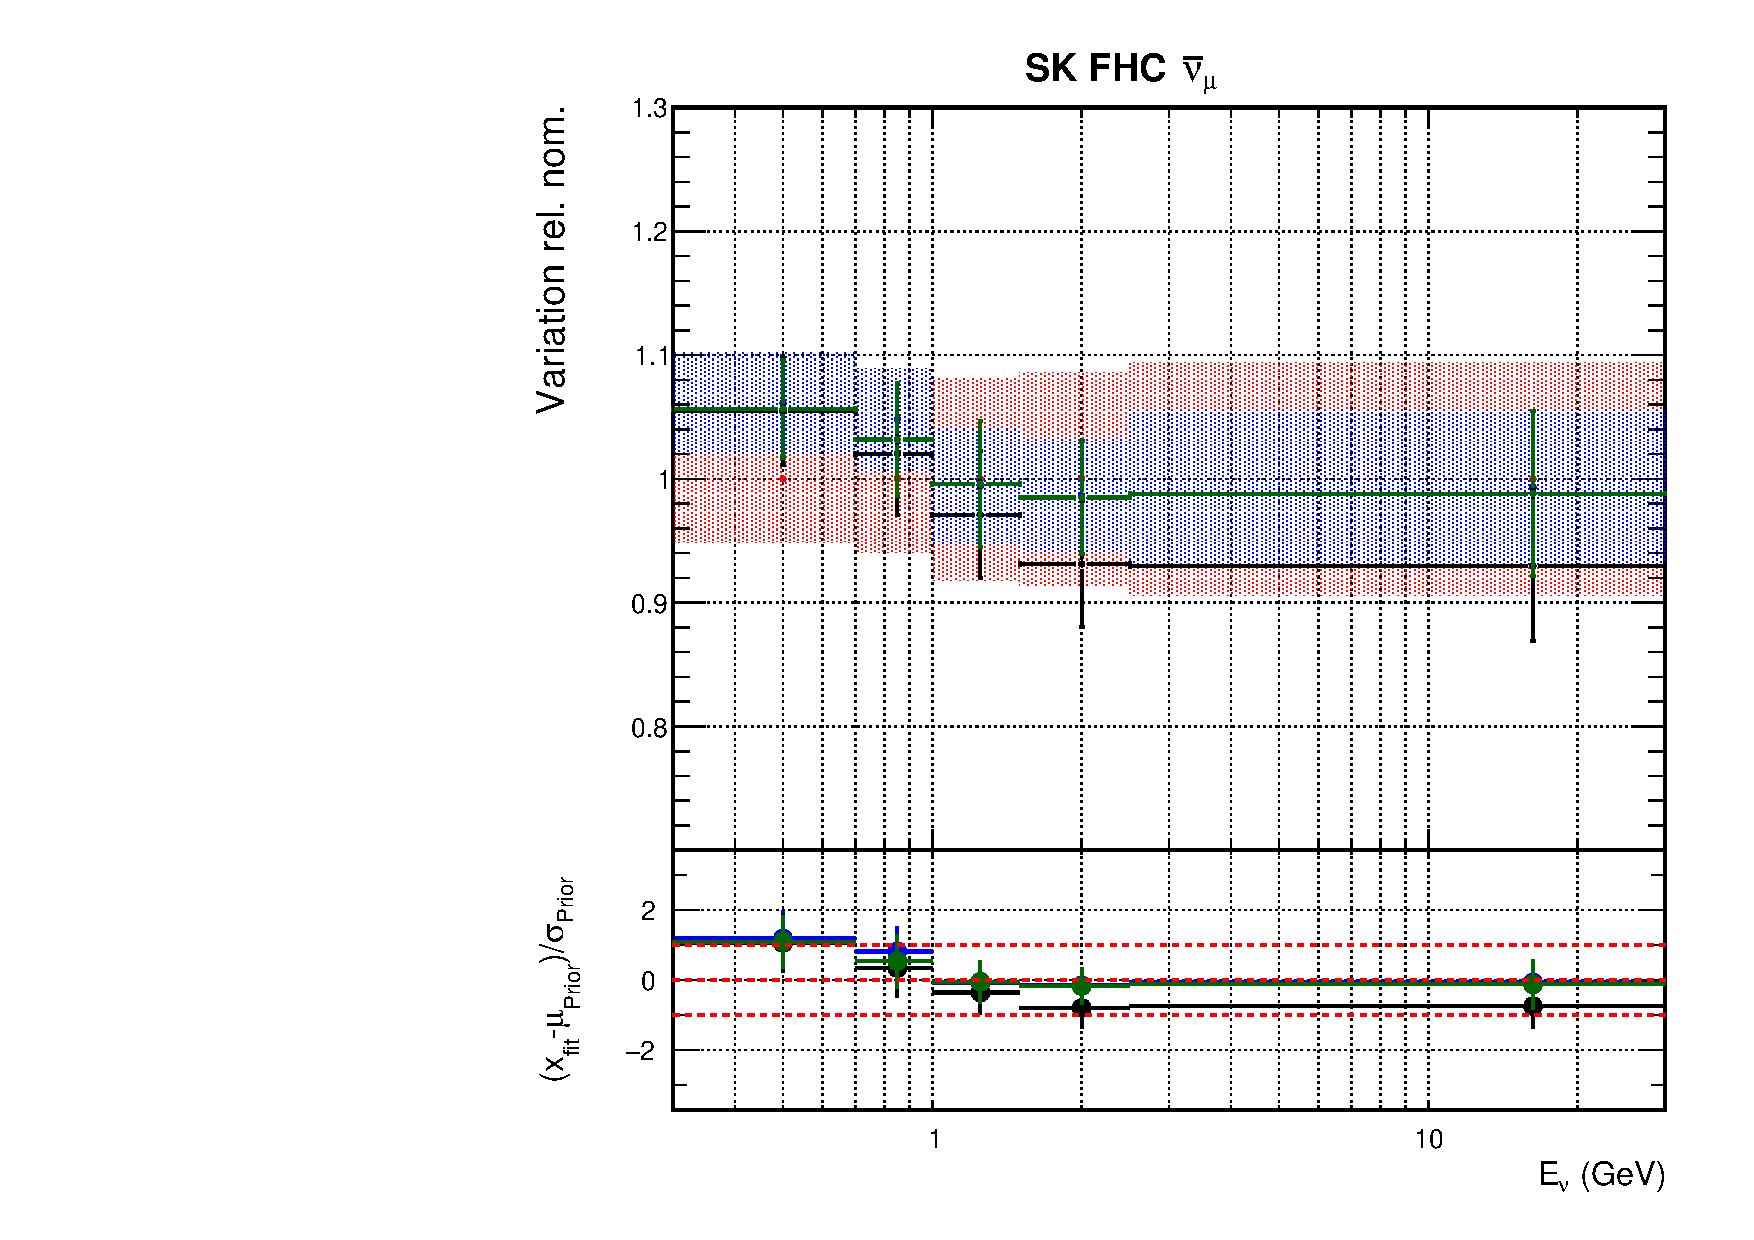
\includegraphics[width=0.75\linewidth]{figs/fgdfitsflux_10}
  \caption{\SK FHC $\nu_e$}
\end{subfigure}
\begin{subfigure}{0.45\textwidth}
  \centering
  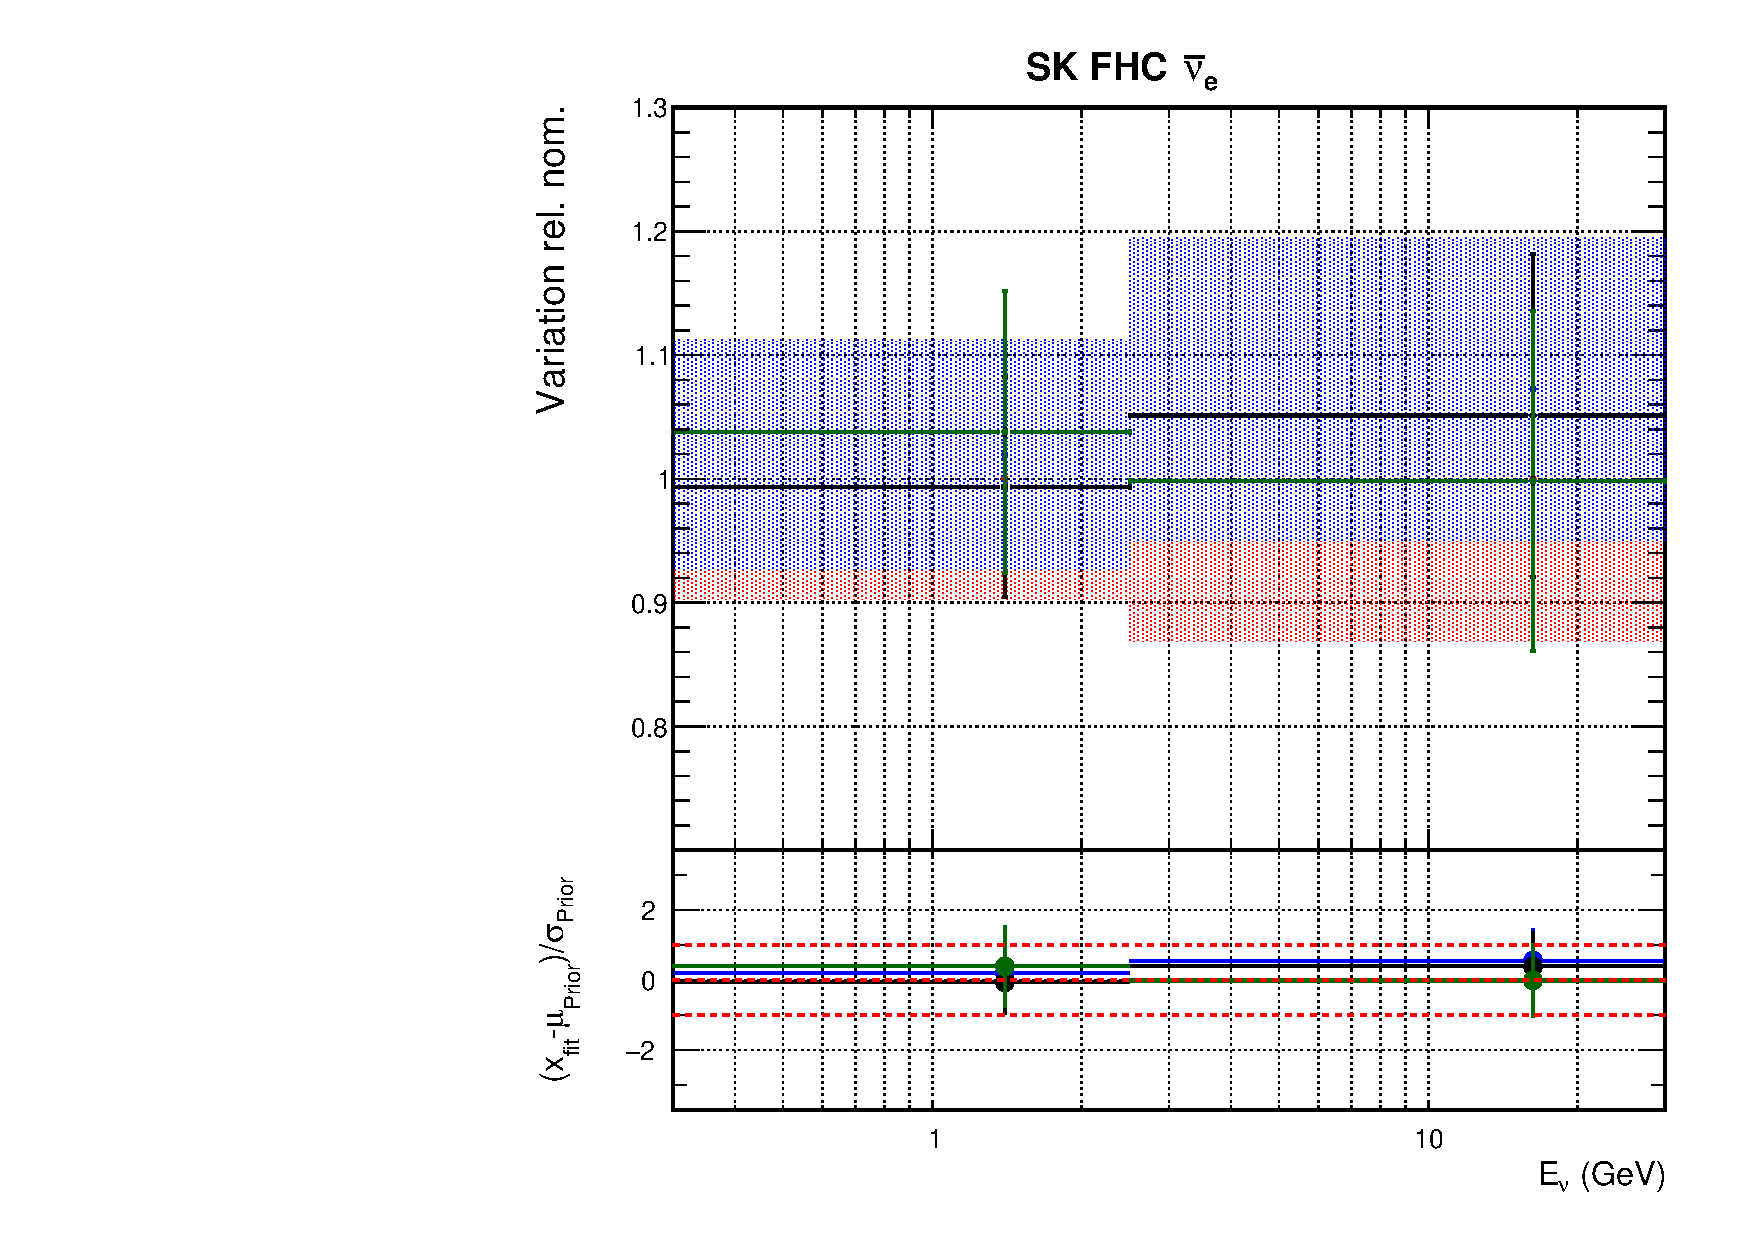
\includegraphics[width=0.75\linewidth]{figs/fgdfitsflux_11}
  \caption{\SK FHC $\bar{\nu_{e}}$}
\end{subfigure}
\begin{subfigure}{0.45\textwidth}
  \centering
  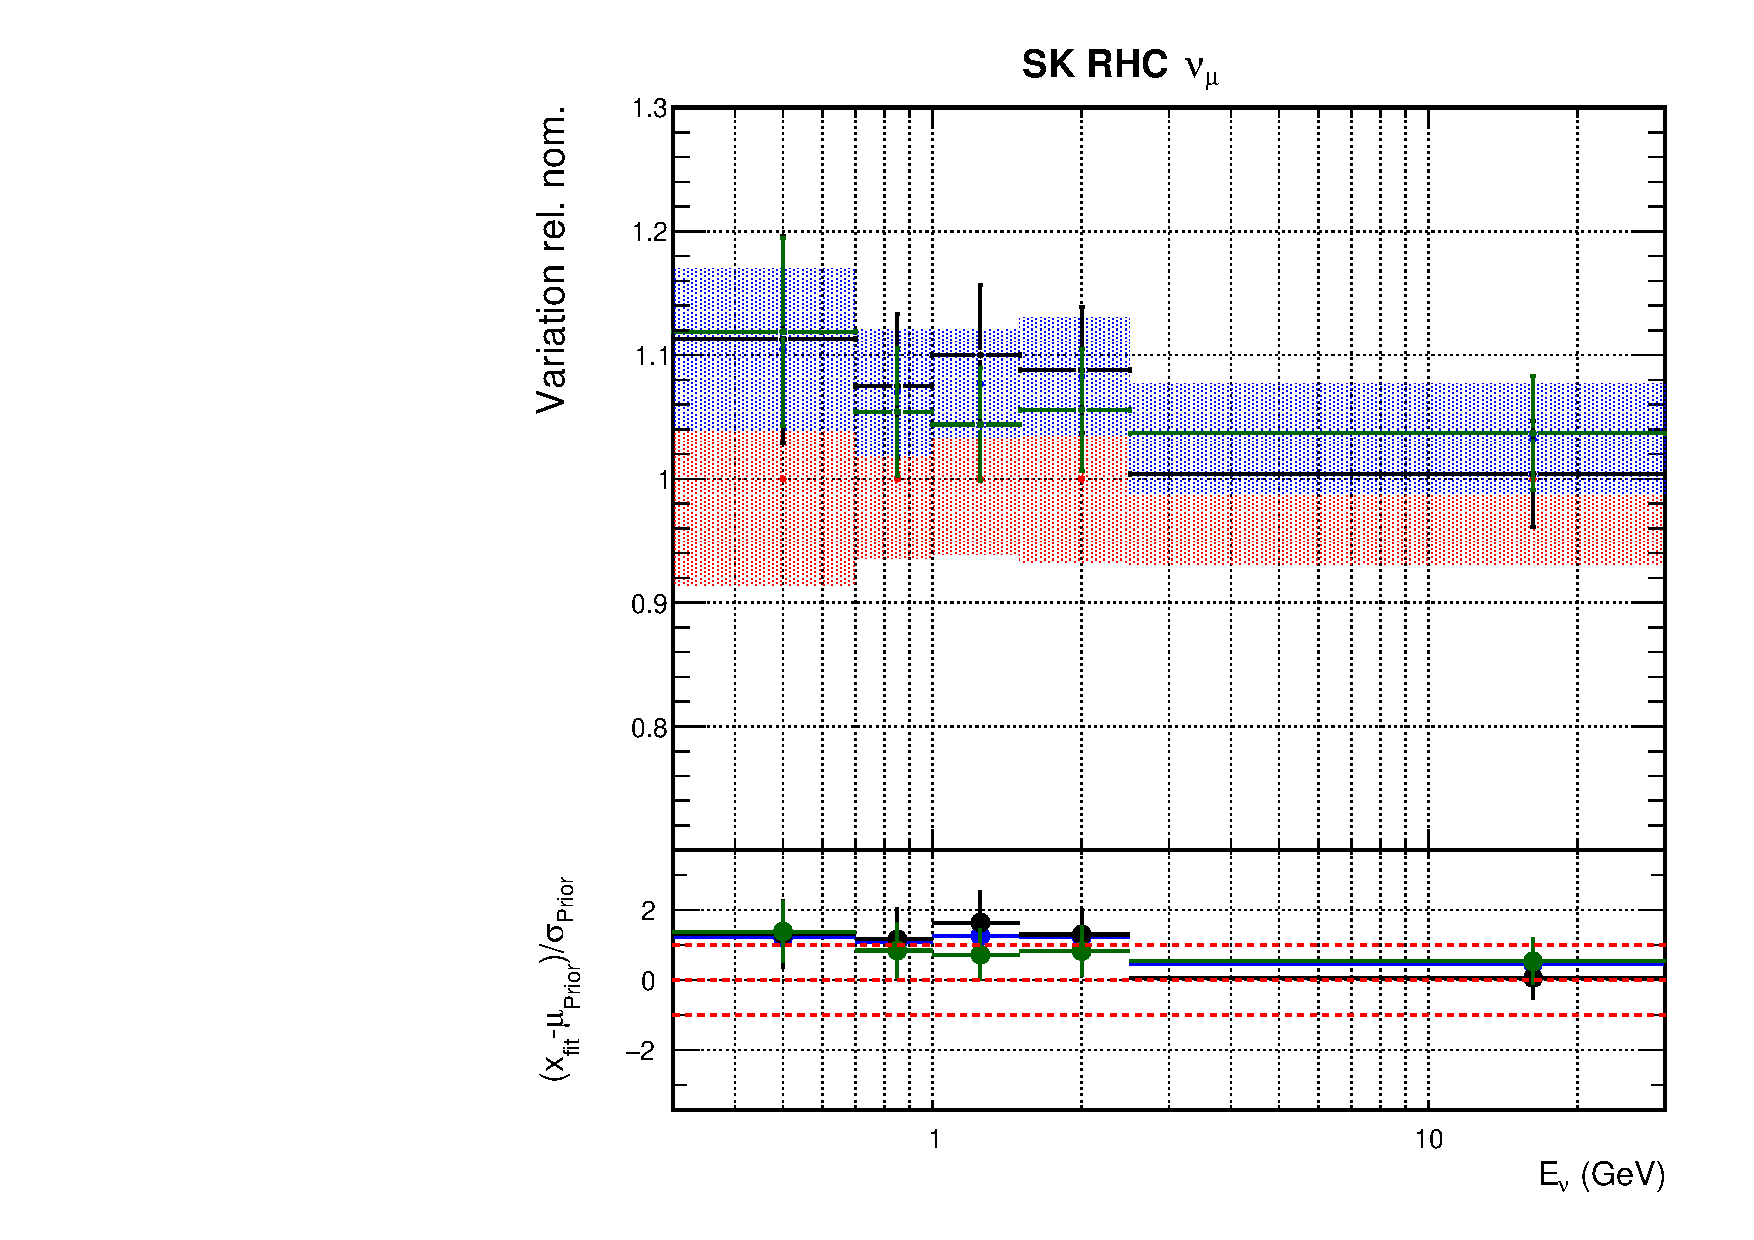
\includegraphics[width=0.75\linewidth]{figs/fgdfitsflux_12}
  \caption{\SK RHC $\nu_{\mu}$}
\end{subfigure}
\begin{subfigure}{0.45\textwidth}
  \centering
  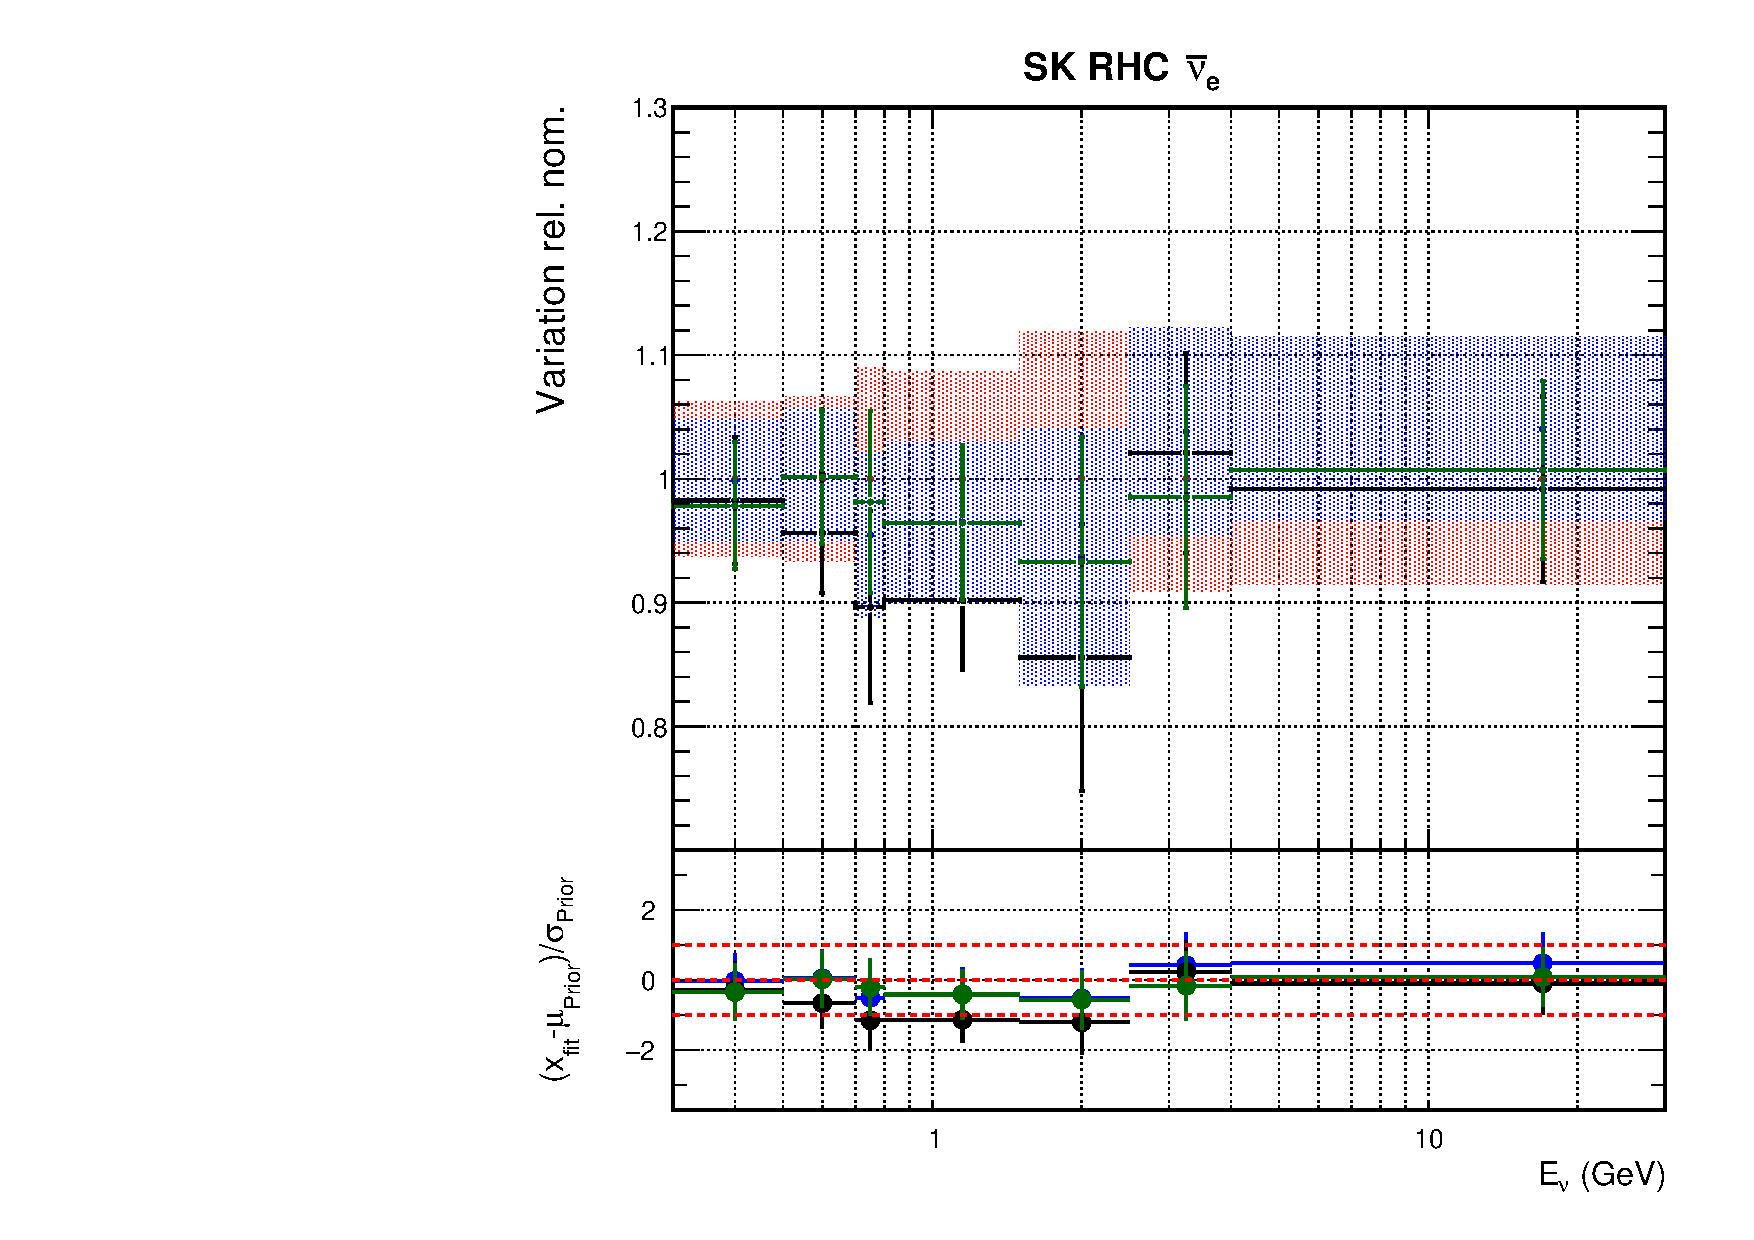
\includegraphics[width=0.75\linewidth]{figs/fgdfitsflux_13}
  \caption{\SK RHC $\bar{\nu_{\mu}}$}
\end{subfigure}
\begin{subfigure}{0.45\textwidth}
  \centering
  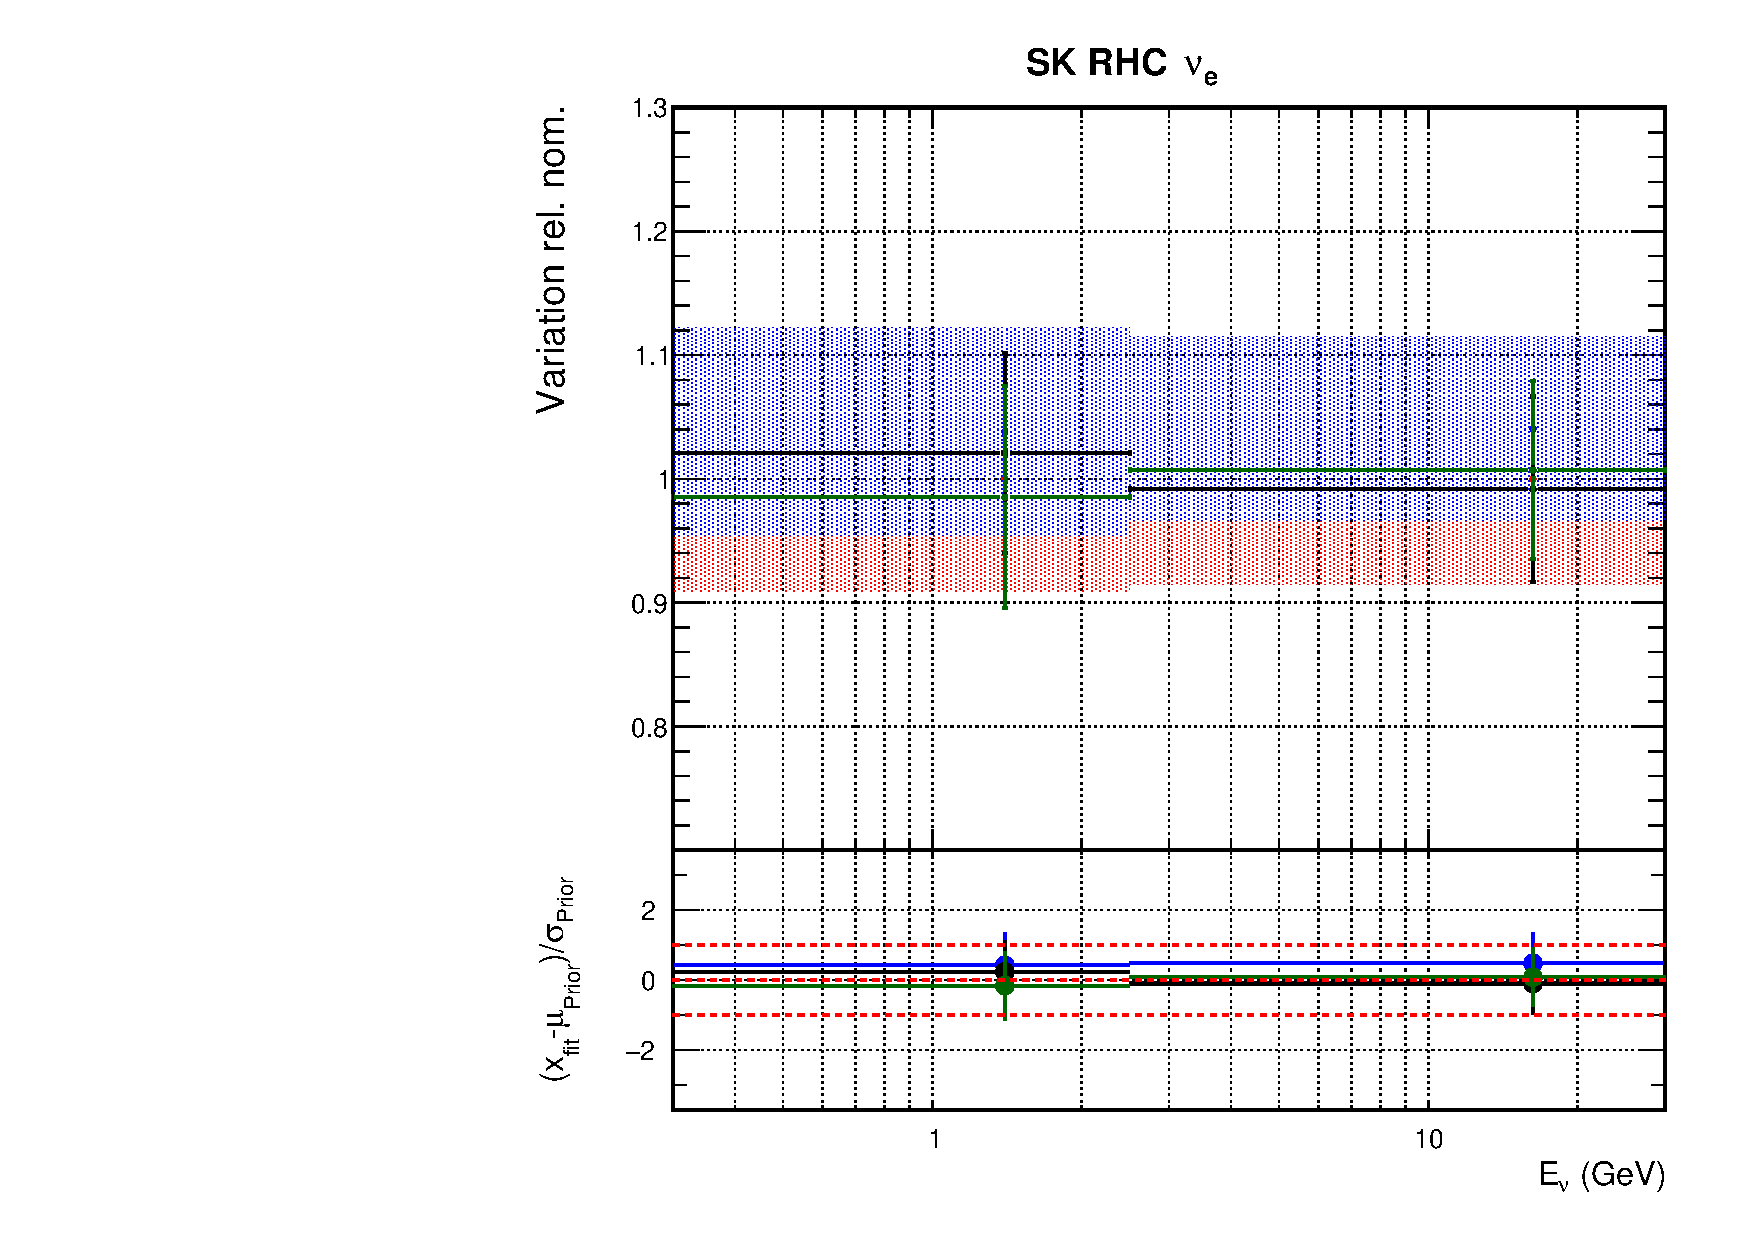
\includegraphics[width=0.75\linewidth]{figs/fgdfitsflux_14}
  \caption{\SK RHC $\nu_{e}$}
\end{subfigure}
\begin{subfigure}{0.45\textwidth}
  \centering
  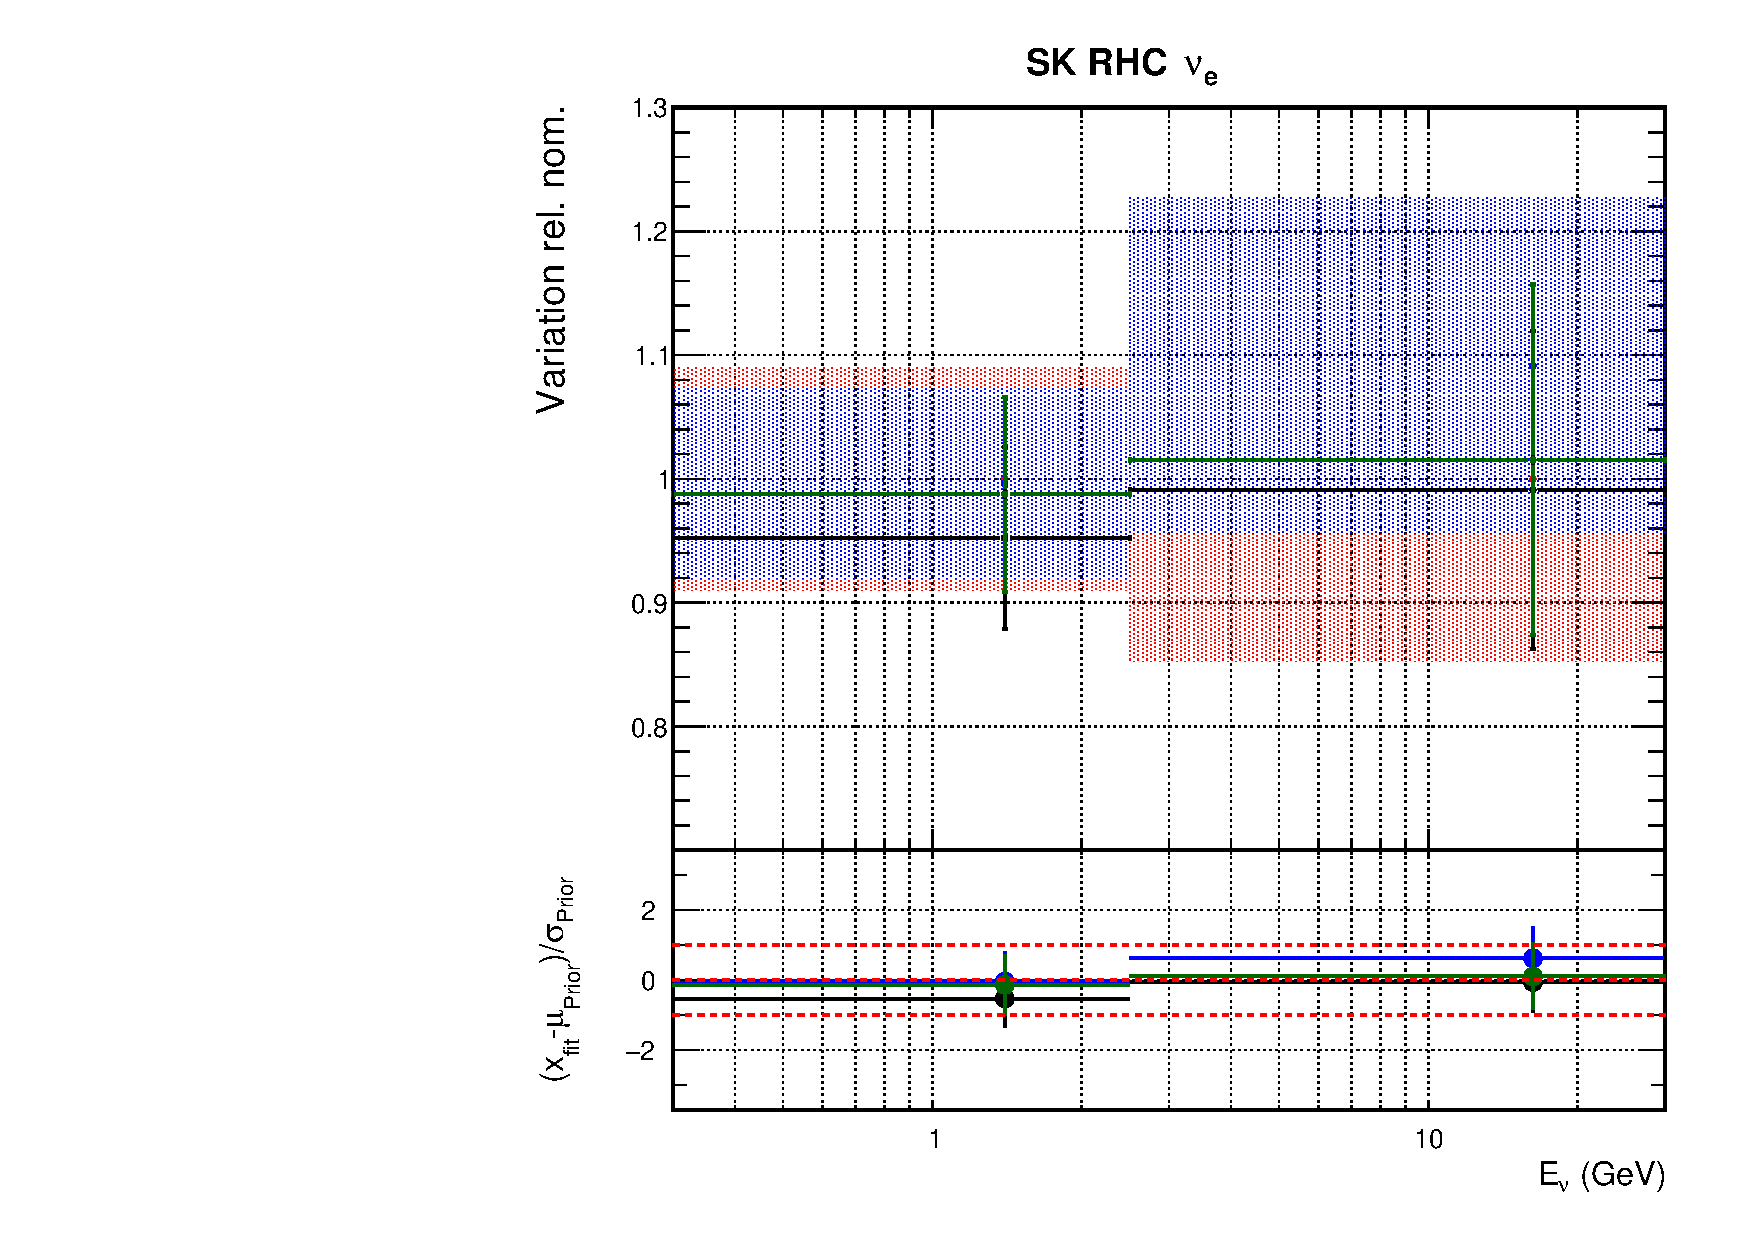
\includegraphics[width=0.75\linewidth]{figs/fgdfitsflux_15}
  \caption{\SK RHC $\bar{\nu_e}$}
\end{subfigure}
\caption{\SK flux parameters for the FGD1 and 2 only fits.}
\label{fig:fgdfluxSK}
\end{figure}

\begin{figure}
\centering
\begin{subfigure}{0.3\textwidth}
  \centering
  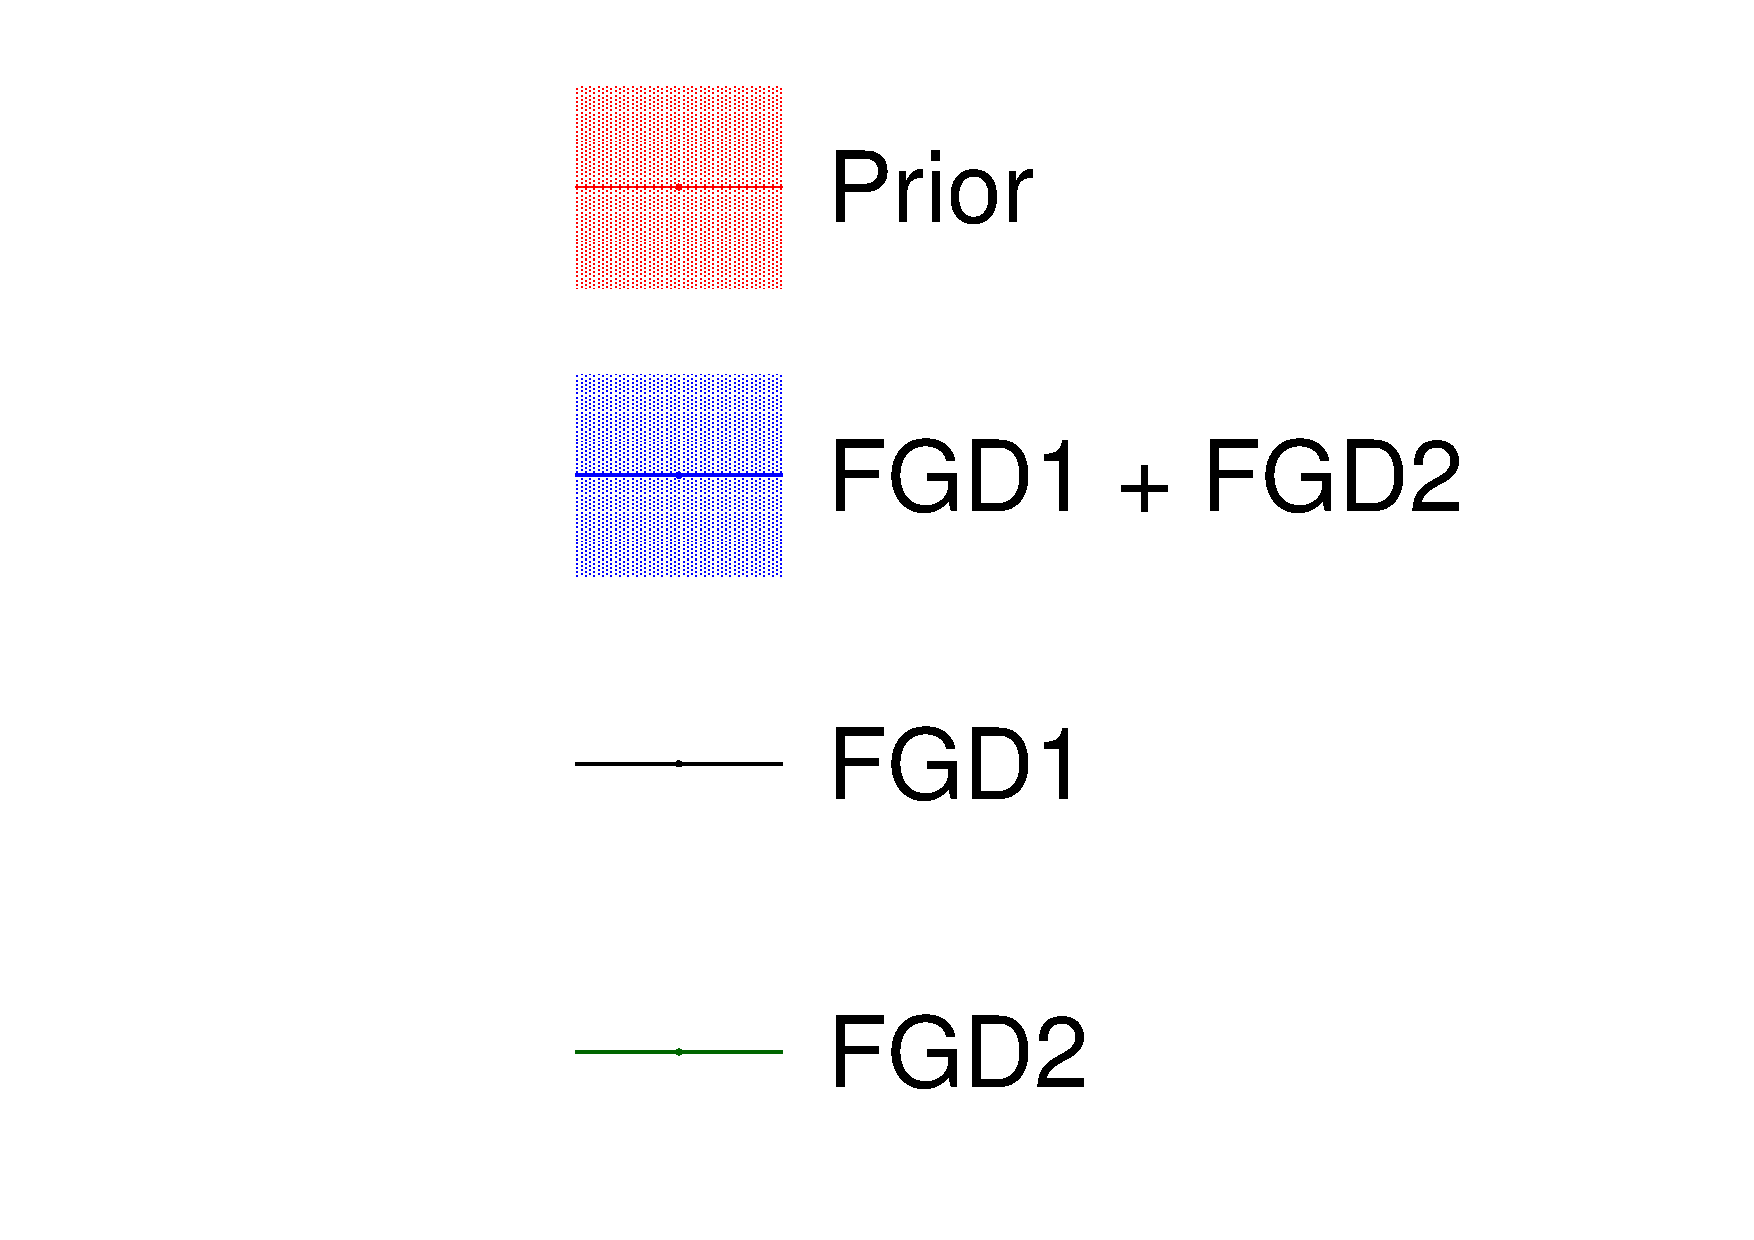
\includegraphics[width=1.0\linewidth, trim={5mm  90mm 0mm 0mm}, clip]{figs/fgdfits_leg}
\end{subfigure}
\begin{subfigure}{0.3\textwidth}
  \centering
  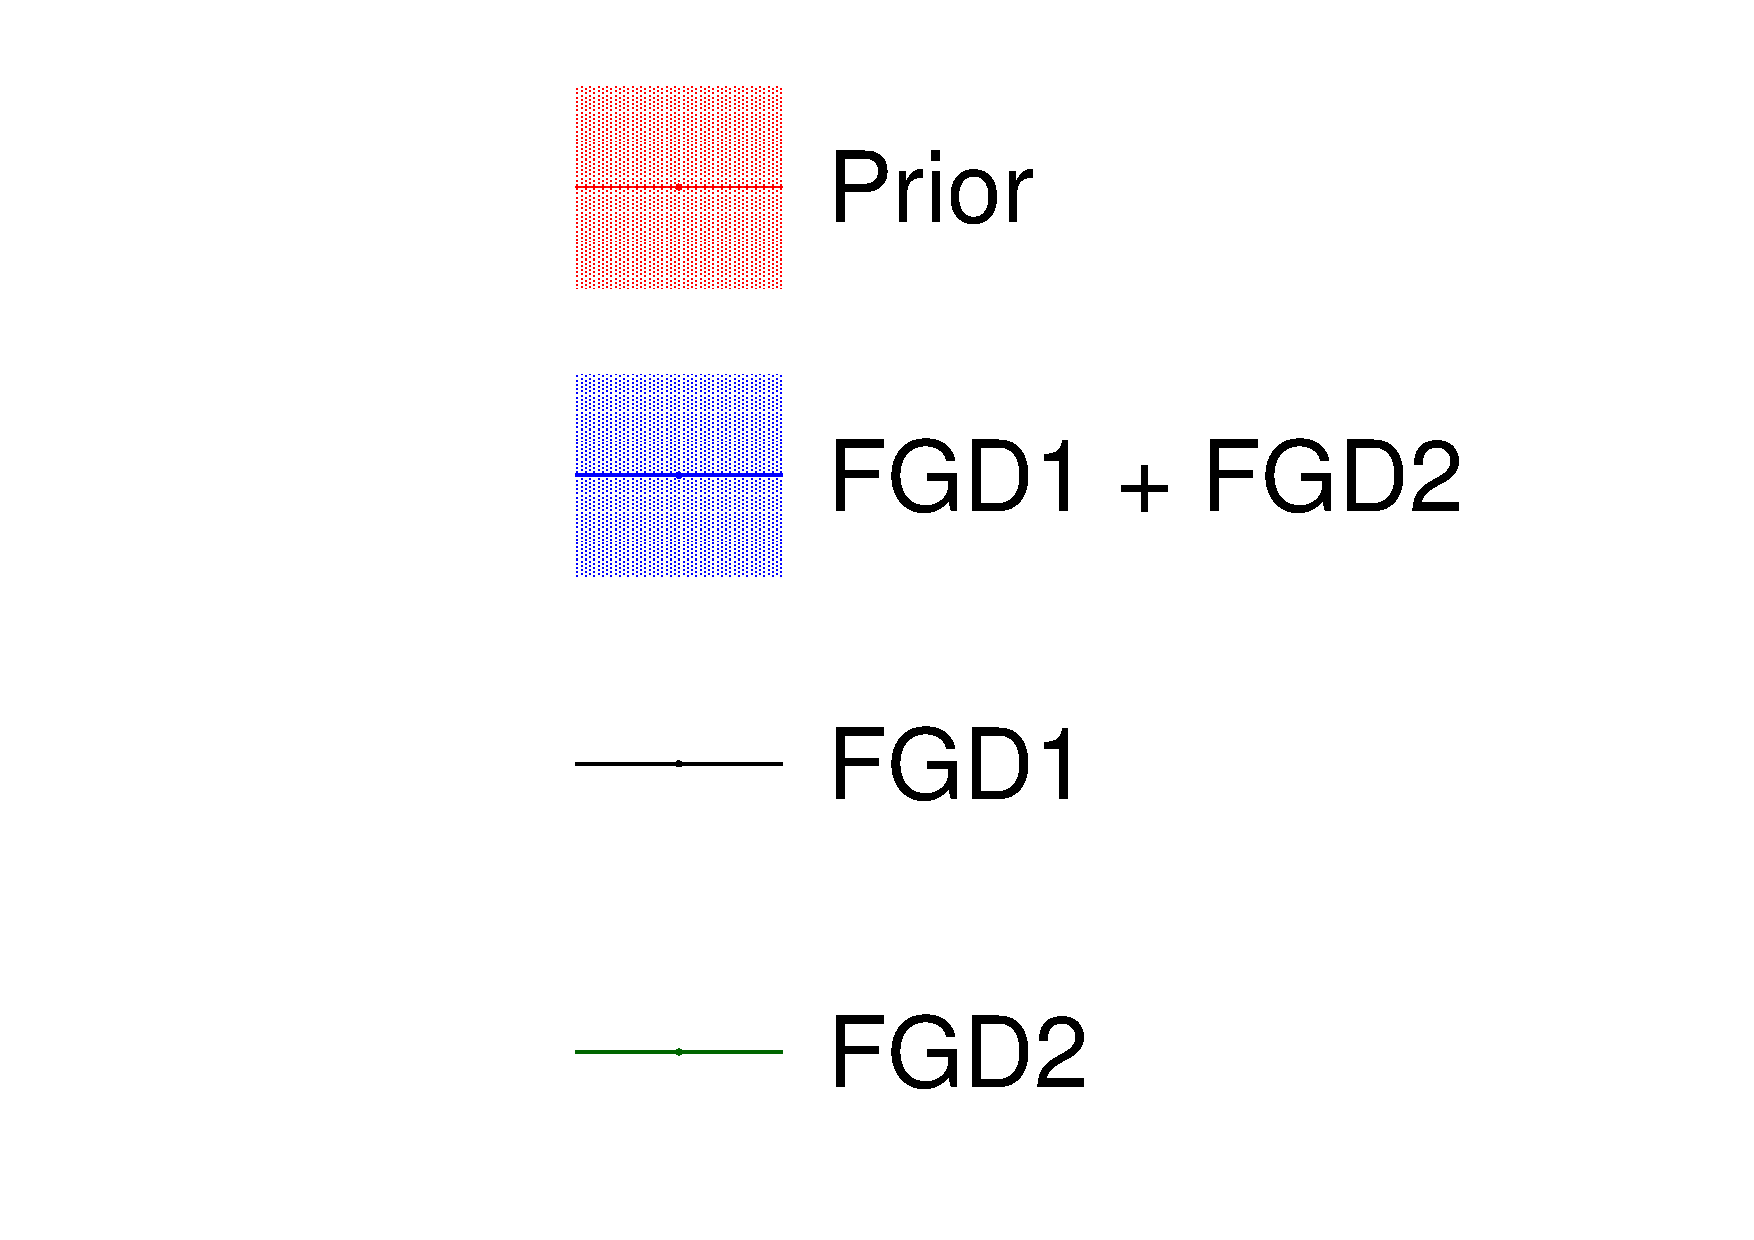
\includegraphics[width=1.0\linewidth, trim={5mm  0mm 0mm 95mm}, clip]{figs/fgdfits_leg}
\end{subfigure}
\begin{subfigure}{0.49\textwidth}
  \centering
  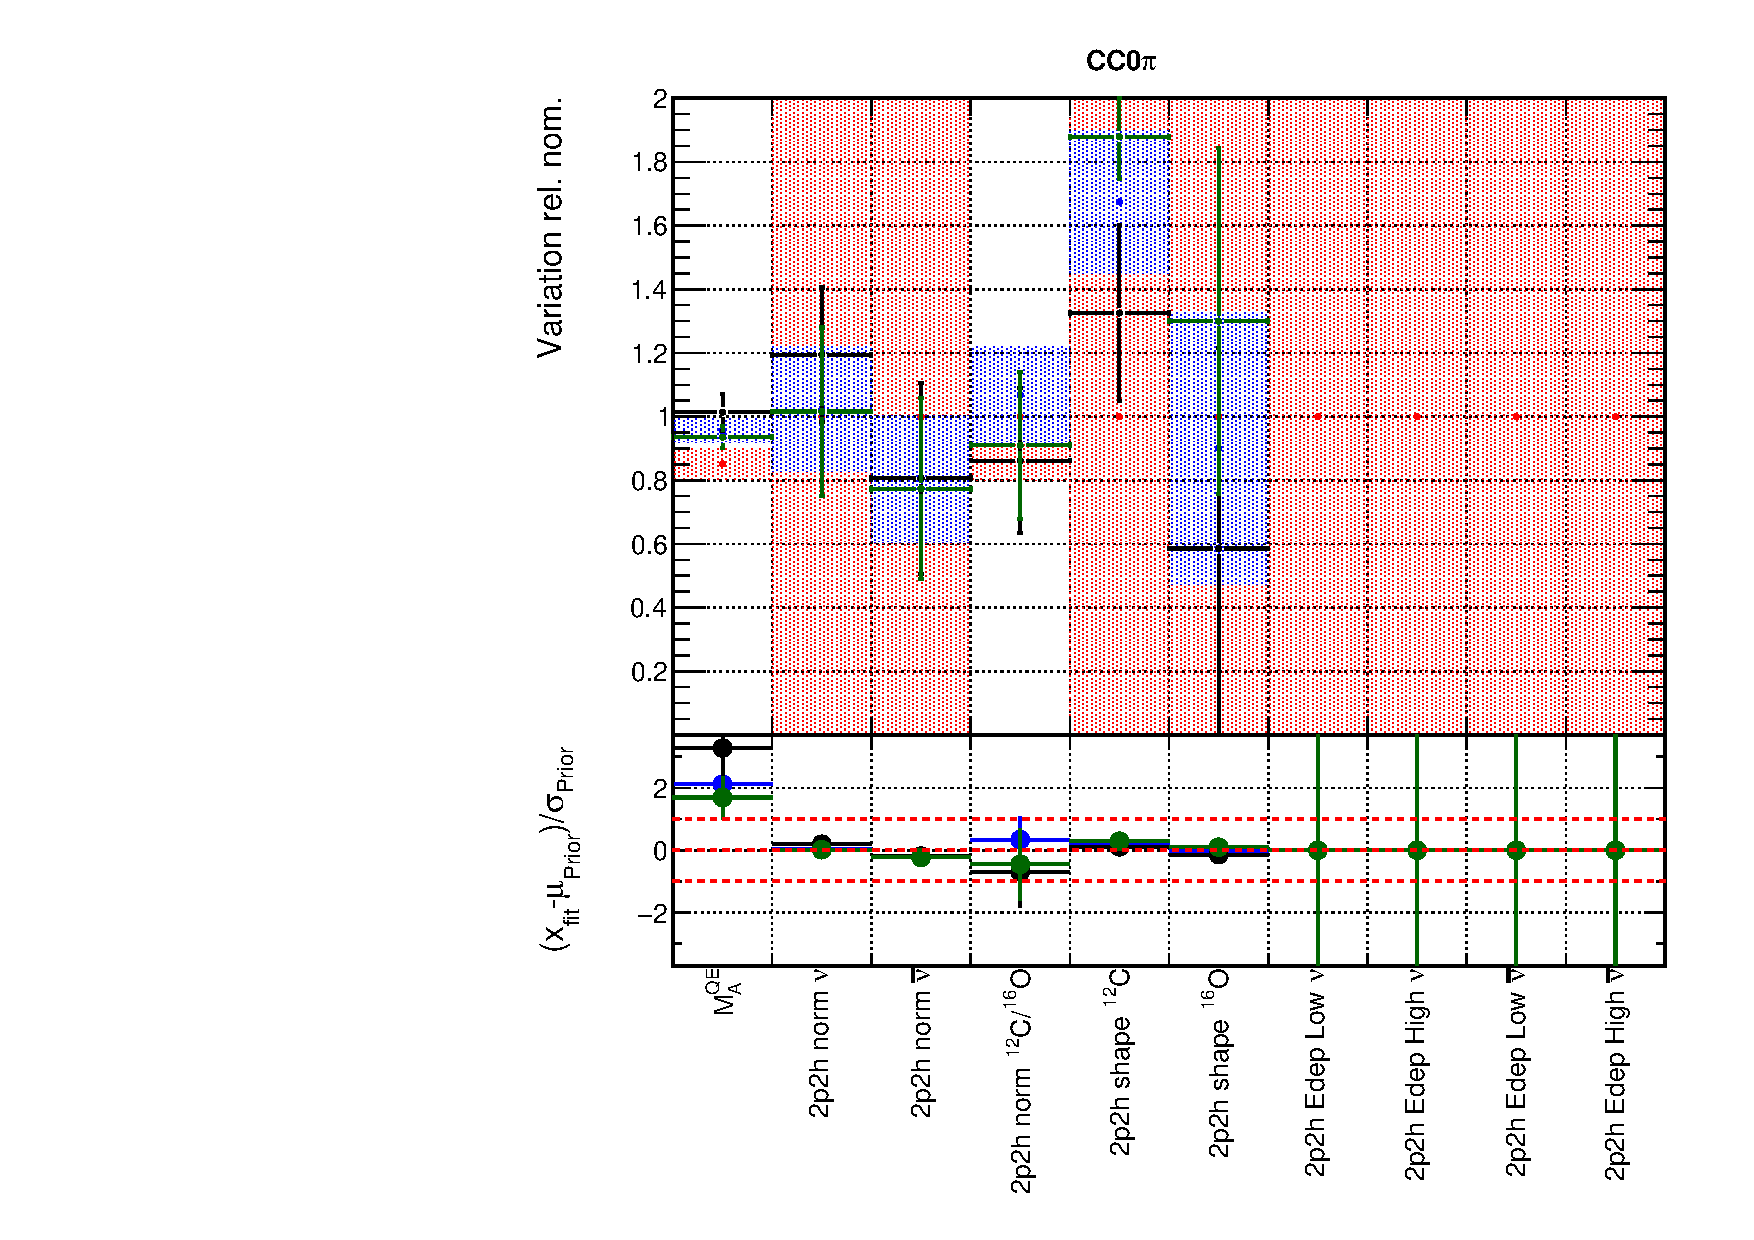
\includegraphics[width=0.9\linewidth]{figs/fgdfitsxsec_1}
  \caption{CC 0$\pi$}
\end{subfigure}
\begin{subfigure}{0.49\textwidth}
  \centering
  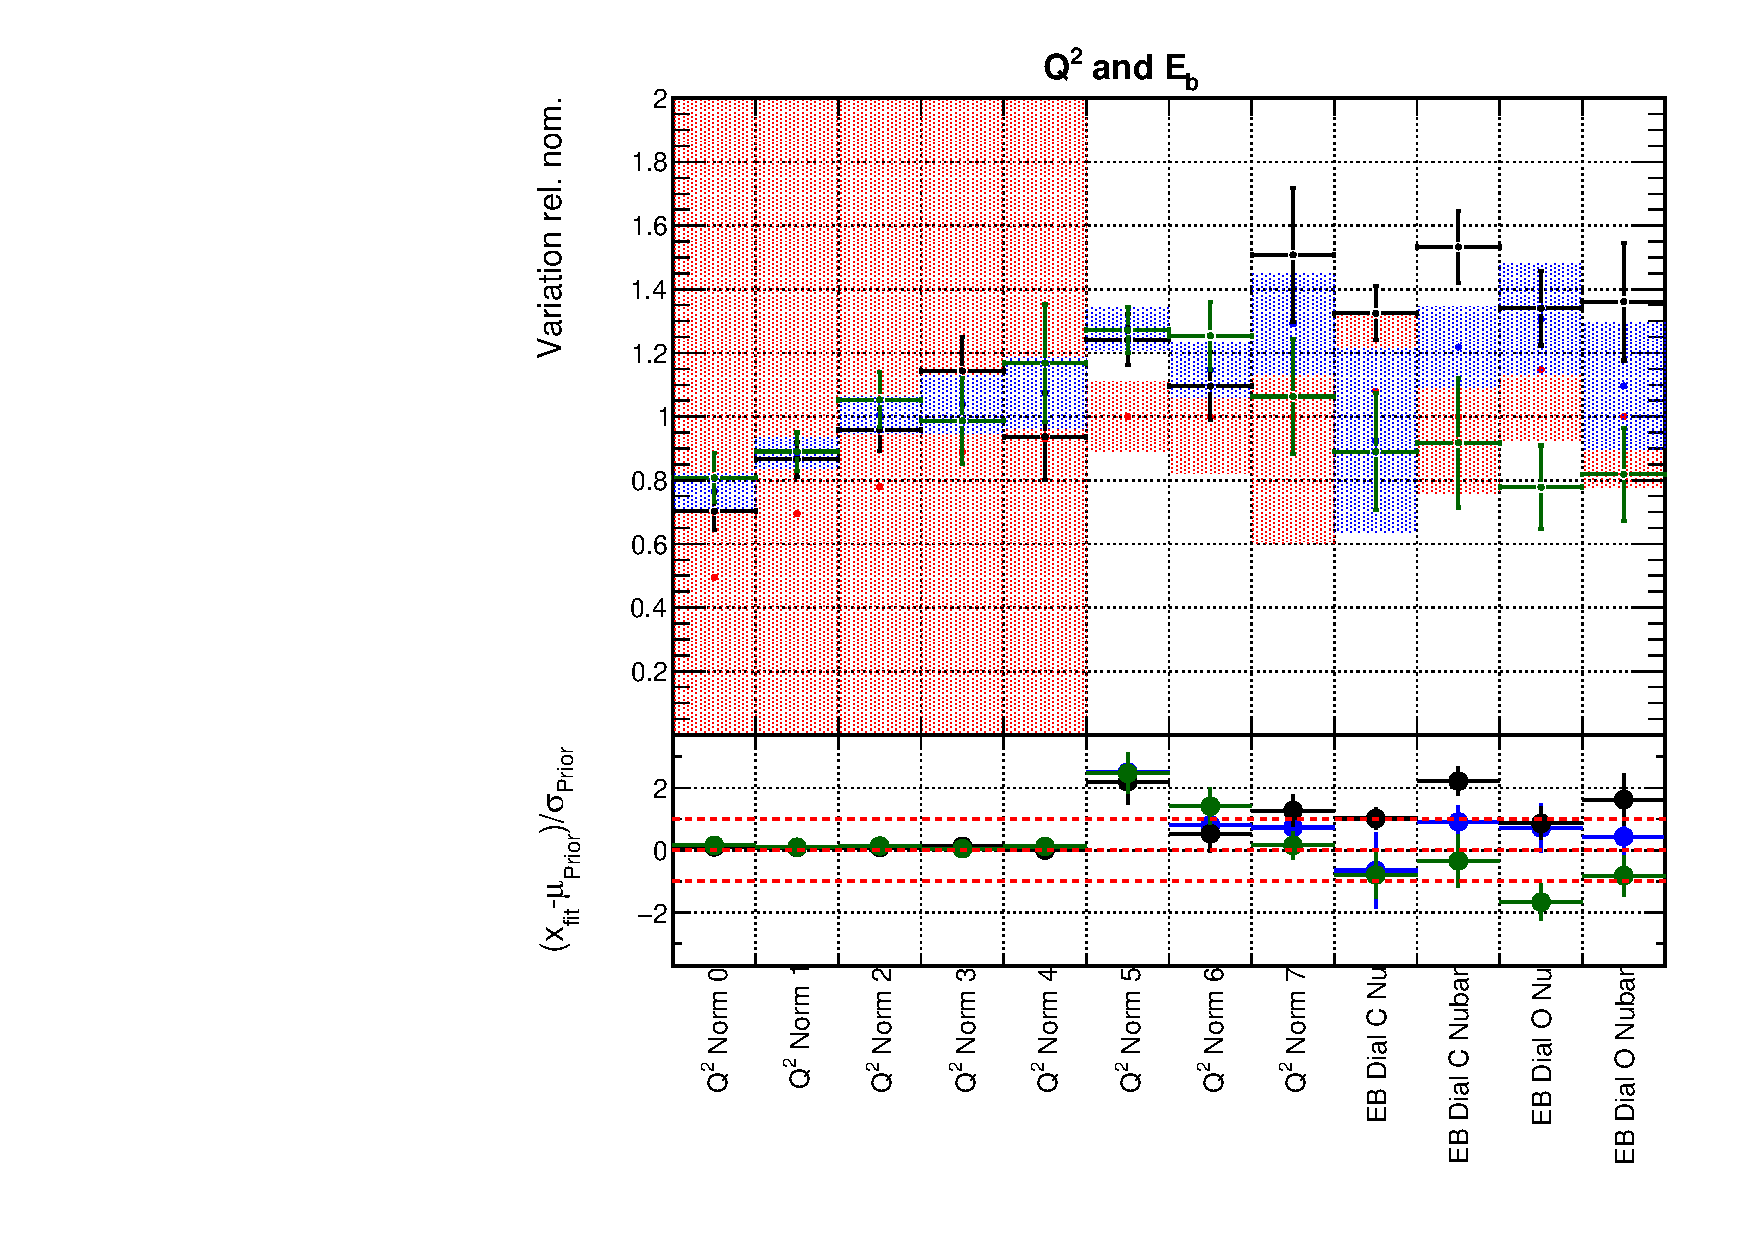
\includegraphics[width=0.9\linewidth]{figs/fgdfitsxsec_2}
  \caption{$Q^2$ and $E_{\mathrm{b}}$}
\end{subfigure}
\begin{subfigure}{0.49\textwidth}
  \centering
  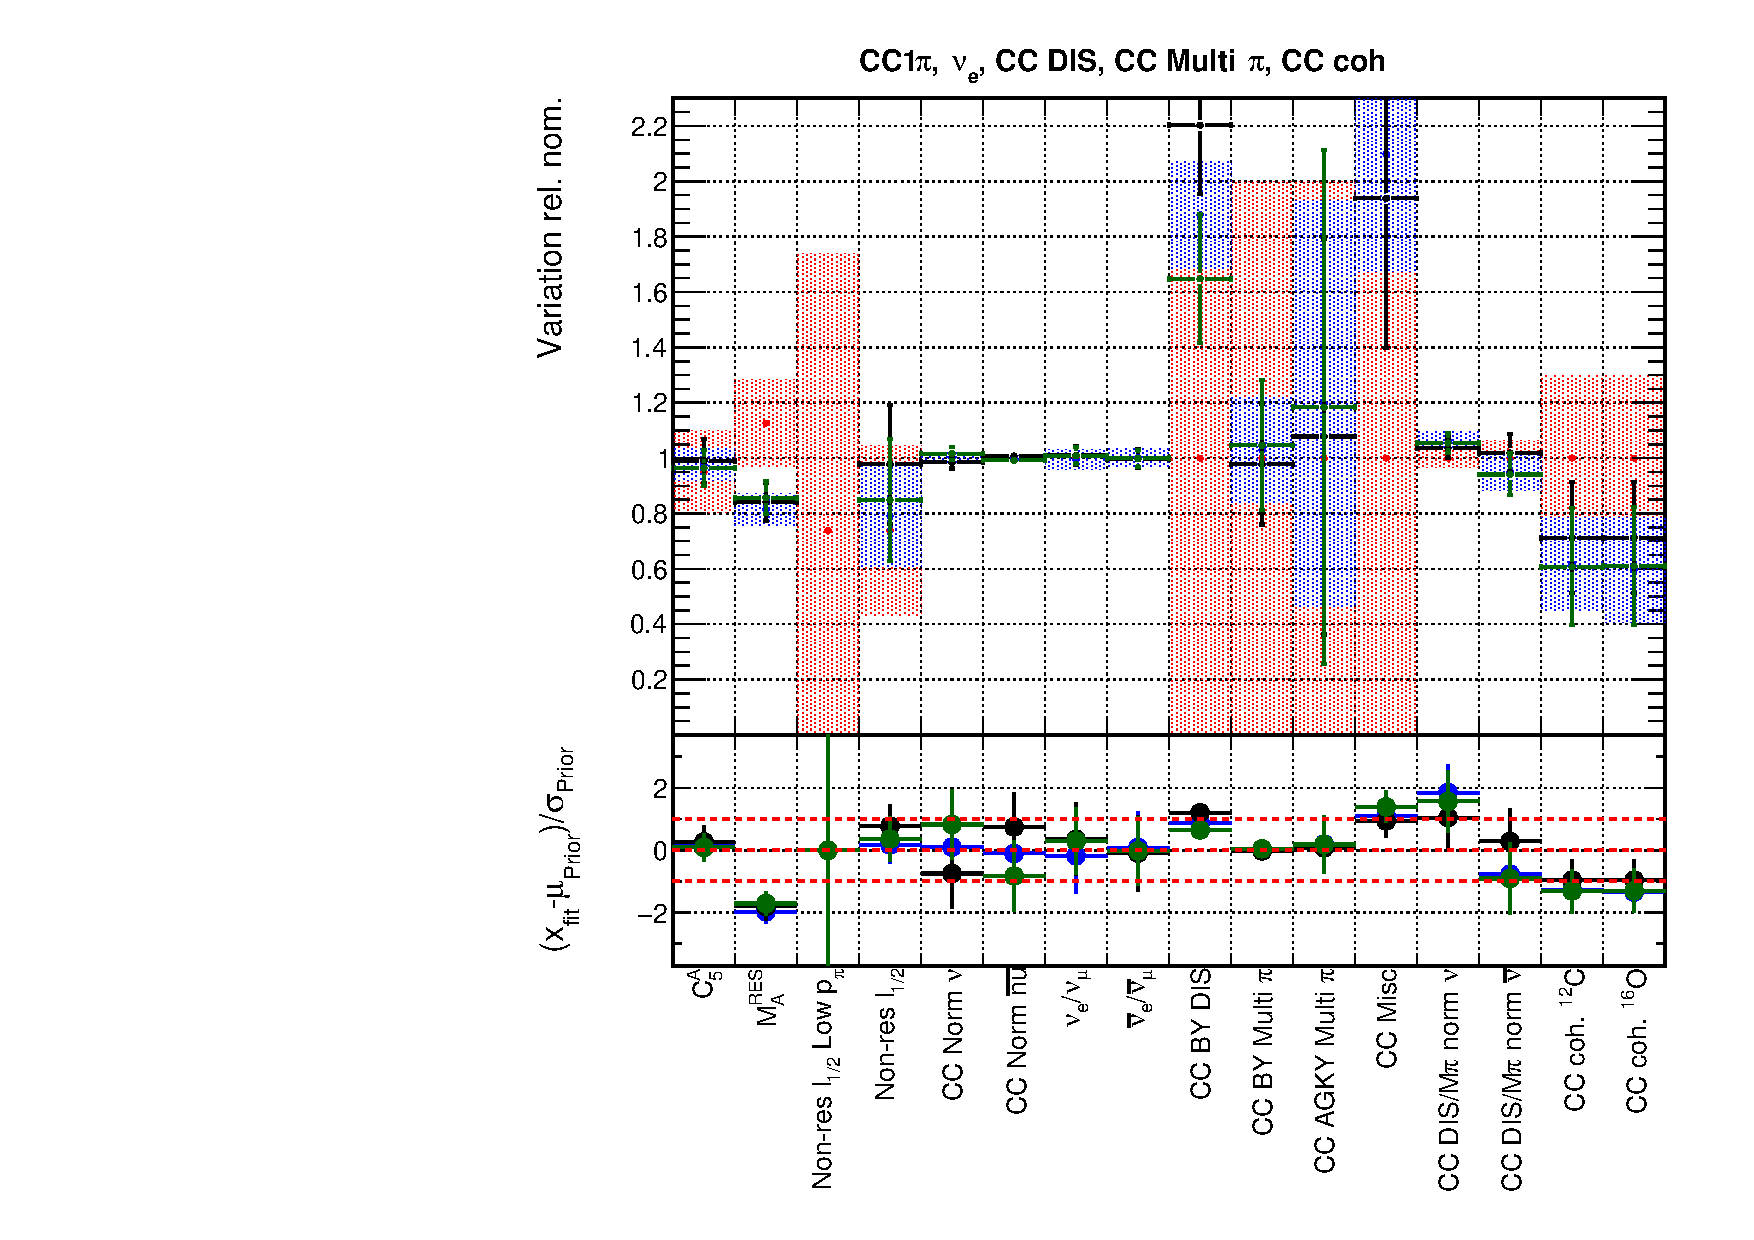
\includegraphics[width=0.9\linewidth]{figs/fgdfitsxsec_3}
  \caption{CC 1$\pi$, $\nu_e$, CC DIS, CC multi-$\pi$ and CC Coh.}
\end{subfigure}
\begin{subfigure}{0.49\textwidth}
  \centering
  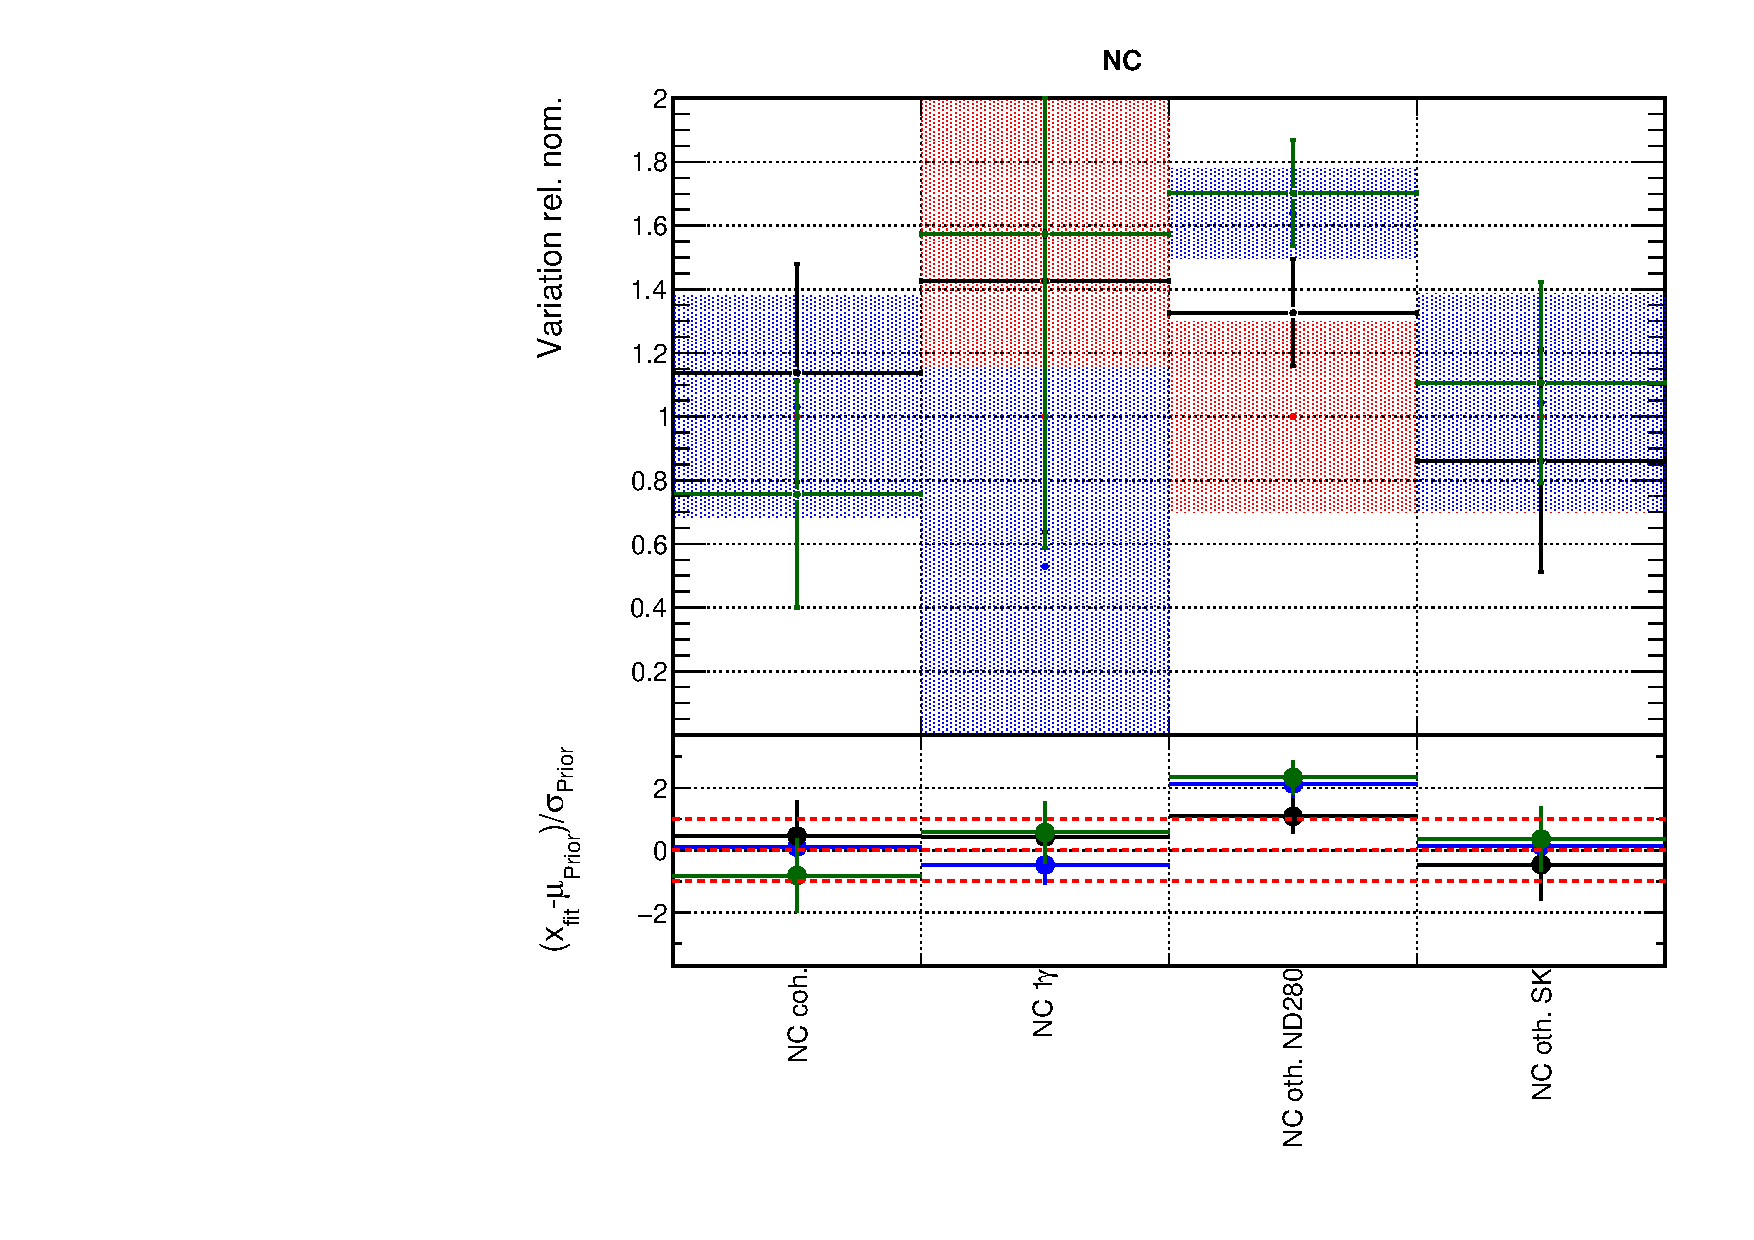
\includegraphics[width=0.9\linewidth]{figs/fgdfitsxsec_4}
  \caption{NC}
\end{subfigure}
\begin{subfigure}{0.49\textwidth}
  \centering
  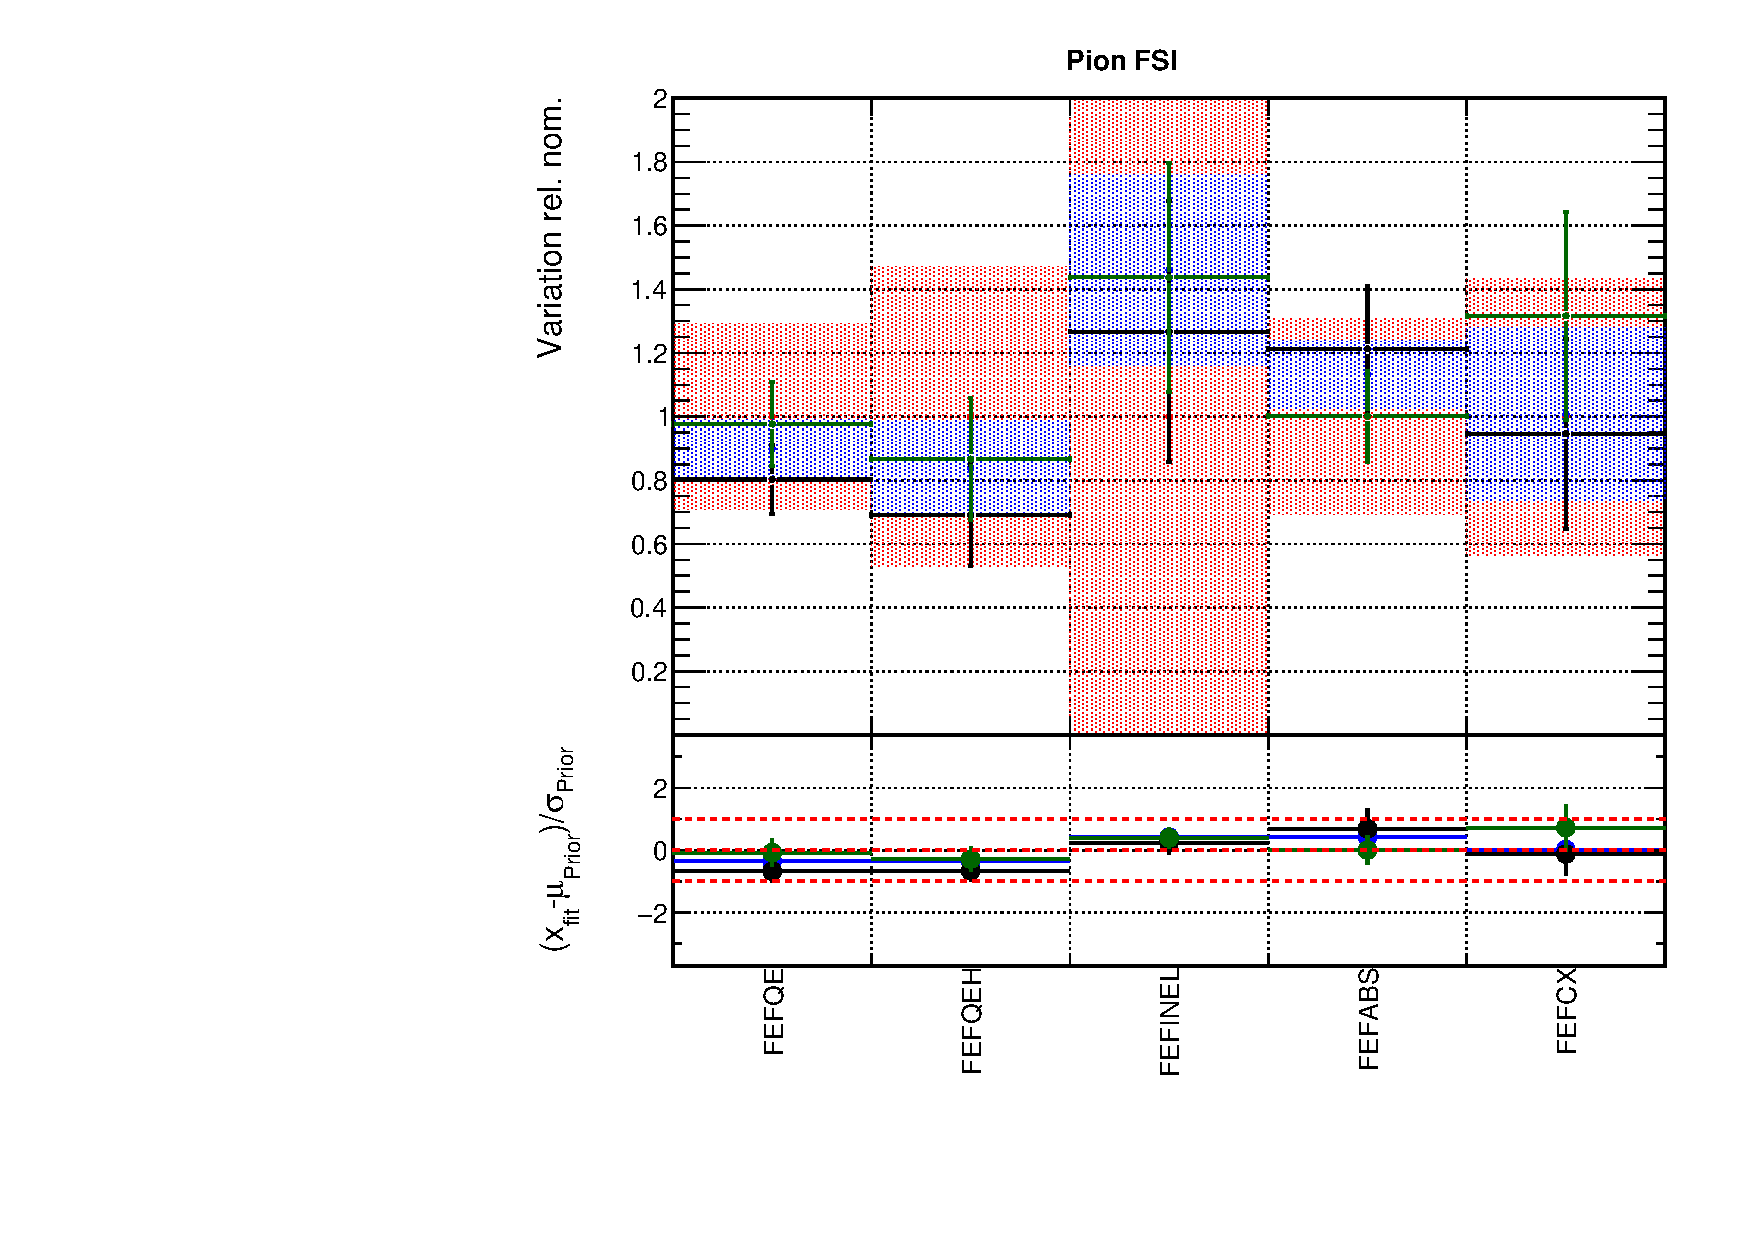
\includegraphics[width=0.9\linewidth]{figs/fgdfitsxsec_5}
  \caption{$\pi$ FSI}
\end{subfigure}
\caption{Interaction parameters for the FGD1 and 2 only fits.}
\label{fig:fgdxsec}
\end{figure}

The interaction parameters, shown in Figure \ref{fig:FGDEbdata}, have larger differences. $M_{A}^{QE}$ is pushed higher for FGD1 than FGD2, with the full fit value lying between two. The 2p2h $\nu$ normalisation parameter is also higher for FGD1, with the FGD2 value remaining close to nominal as it is for the full fit. The 2p2h shape parameters have large differences. For FGD2, 2p2h shape C is pushed to its upper bound at $\sim$2, whereas it is only pushed to $\sim$1.3 for FGD1. This is interesting as both FGDs are able to constrain the parameter. For the full fit, the 2p2h shape C postfit value lies between the FGD1 and FGD2 values, despite not affecting any FGD1 events. This is likely driven by the prior correlations between 2p2h shape C and O.

The shape of the increase in $Q^2$ parameters is slightly different between the FGD1 and FGD2 fits, but all are within uncertainty of each other.

The $E_{\mathrm{b}}$ parameters are significantly higher for FGD1. As discussed in Section \ref{sec:extrac}, as these parameters are non-Gaussian it is important to inspect the full distributions as well as the extracted values. These are shown in Figure \ref{fig:FGDEbdata}. For $E_{\mathrm{b}} \nu$ C, there is clearly a strong peak much higher than for both the FGD2 and full fits. For $E_{\mathrm{b}} \bar{\nu}$ C, there is again a higher peak for FGD1, but the full fit lies between the two subdetector fits. For $E_{\mathrm{b}} \nu$ O there is more overlap between the fits, which is more expected as there is no $^{16}$O in FGD1. However, for $E_{\mathrm{b}} \bar{\nu}$ O, there are different peaks for the different fits, driven by the correlations between the $E_{\mathrm{b}}$ parameters.

The CC DIS BY parameter is higher for FGD1 than FGD2, with the full fit falling between the two. The other CC $1\pi$ and CC Other targetting parameters are more consistent for the two fits. NC 1$\gamma$ and NC Other show some differences, but this is not too concerning as there are low statistics for the interaction modes they affect.

For FSI, the charge exchange parameter has the largest discrepancy, but this is within the postfit uncertainty.

Overall there is fairly good compatibility between the FGD samples. Where there are discrepancies, the full fit value tends to fall between the FGD1 and FGD2 only results. CC DIS BY is the only parameter affecting both $^{12}$C and $^{16}$O events which are not within the uncertainty for the two fits. 

\begin{figure}
\centering
\begin{subfigure}{.48\textwidth}
  \centering
  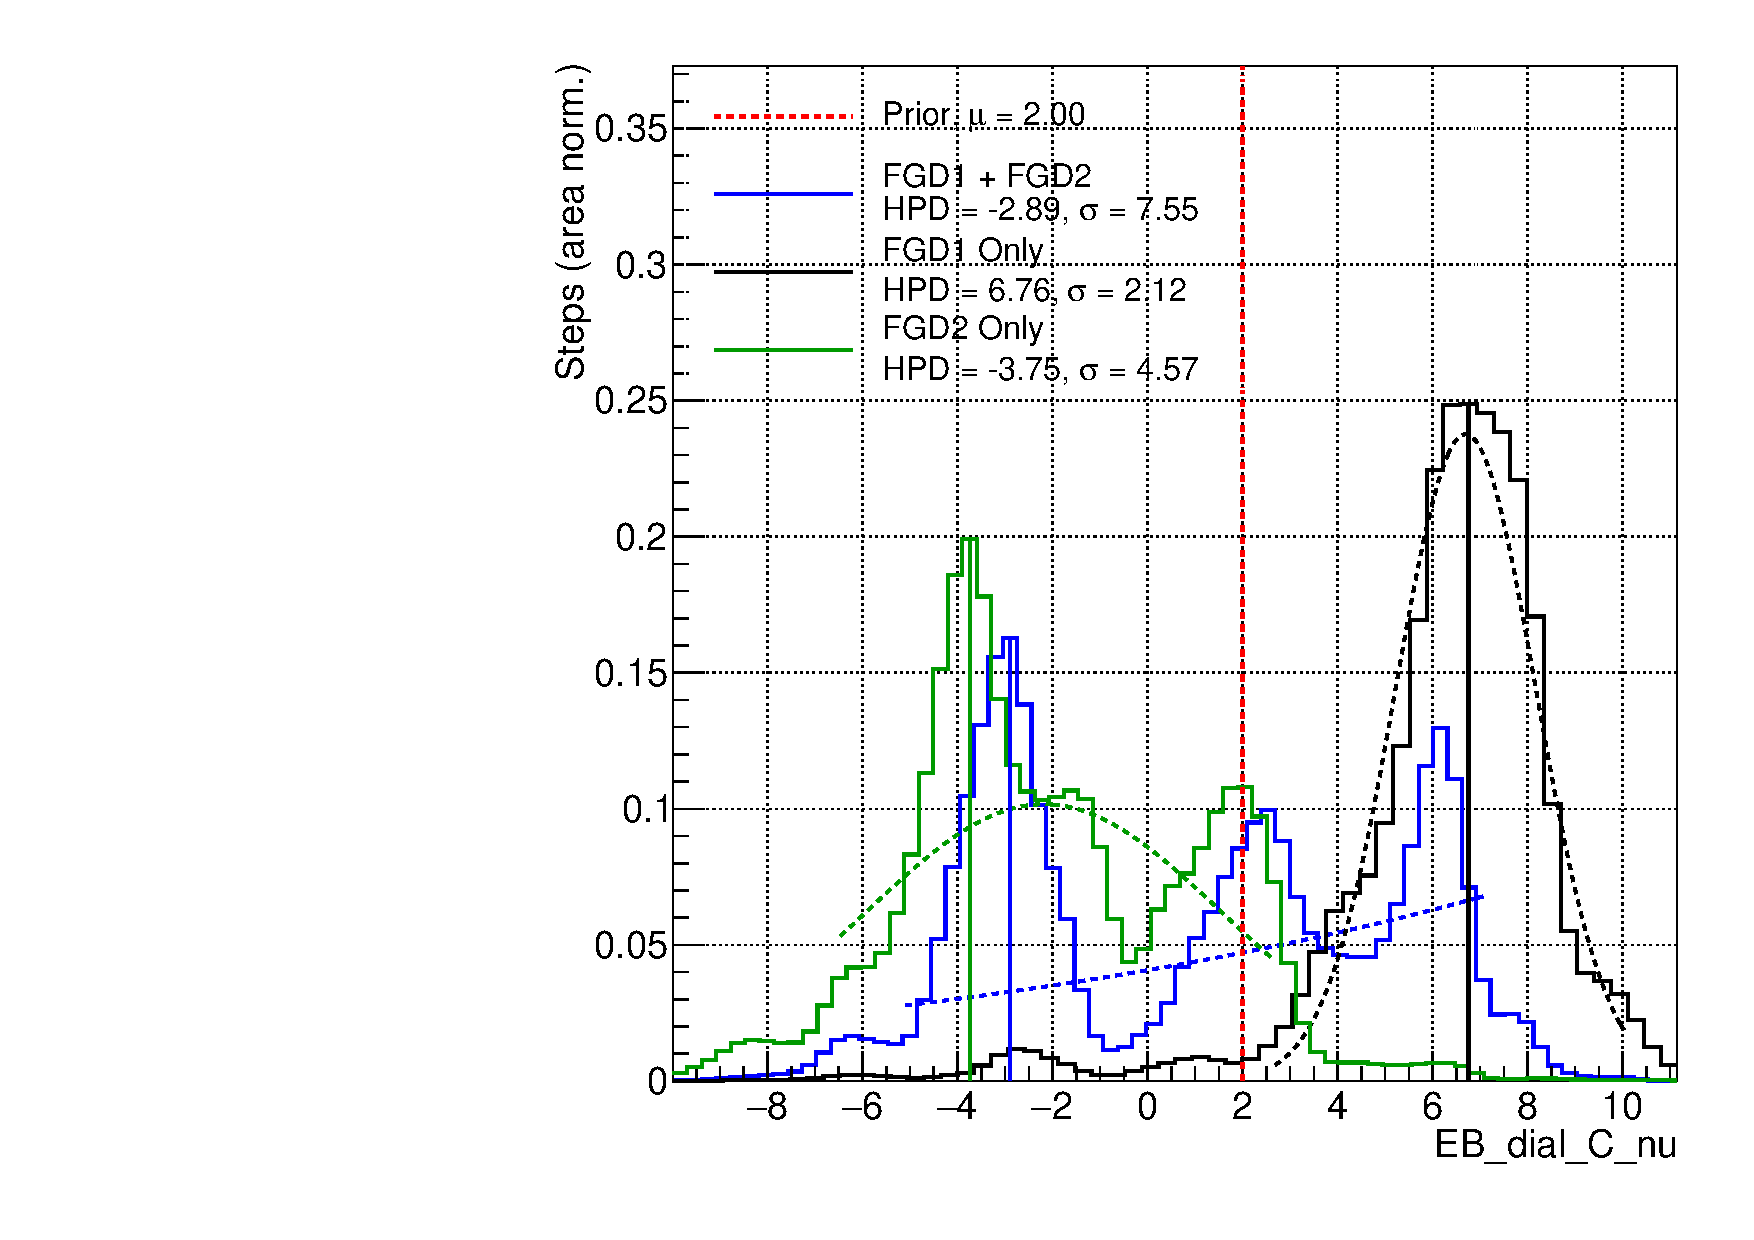
\includegraphics[width=0.73\linewidth]{figs/FGD_EB_dial_C_nu}
  \caption{$E_{\mathrm{b}}\nu$ C}
\end{subfigure}
\begin{subfigure}{.48\textwidth}
  \centering
  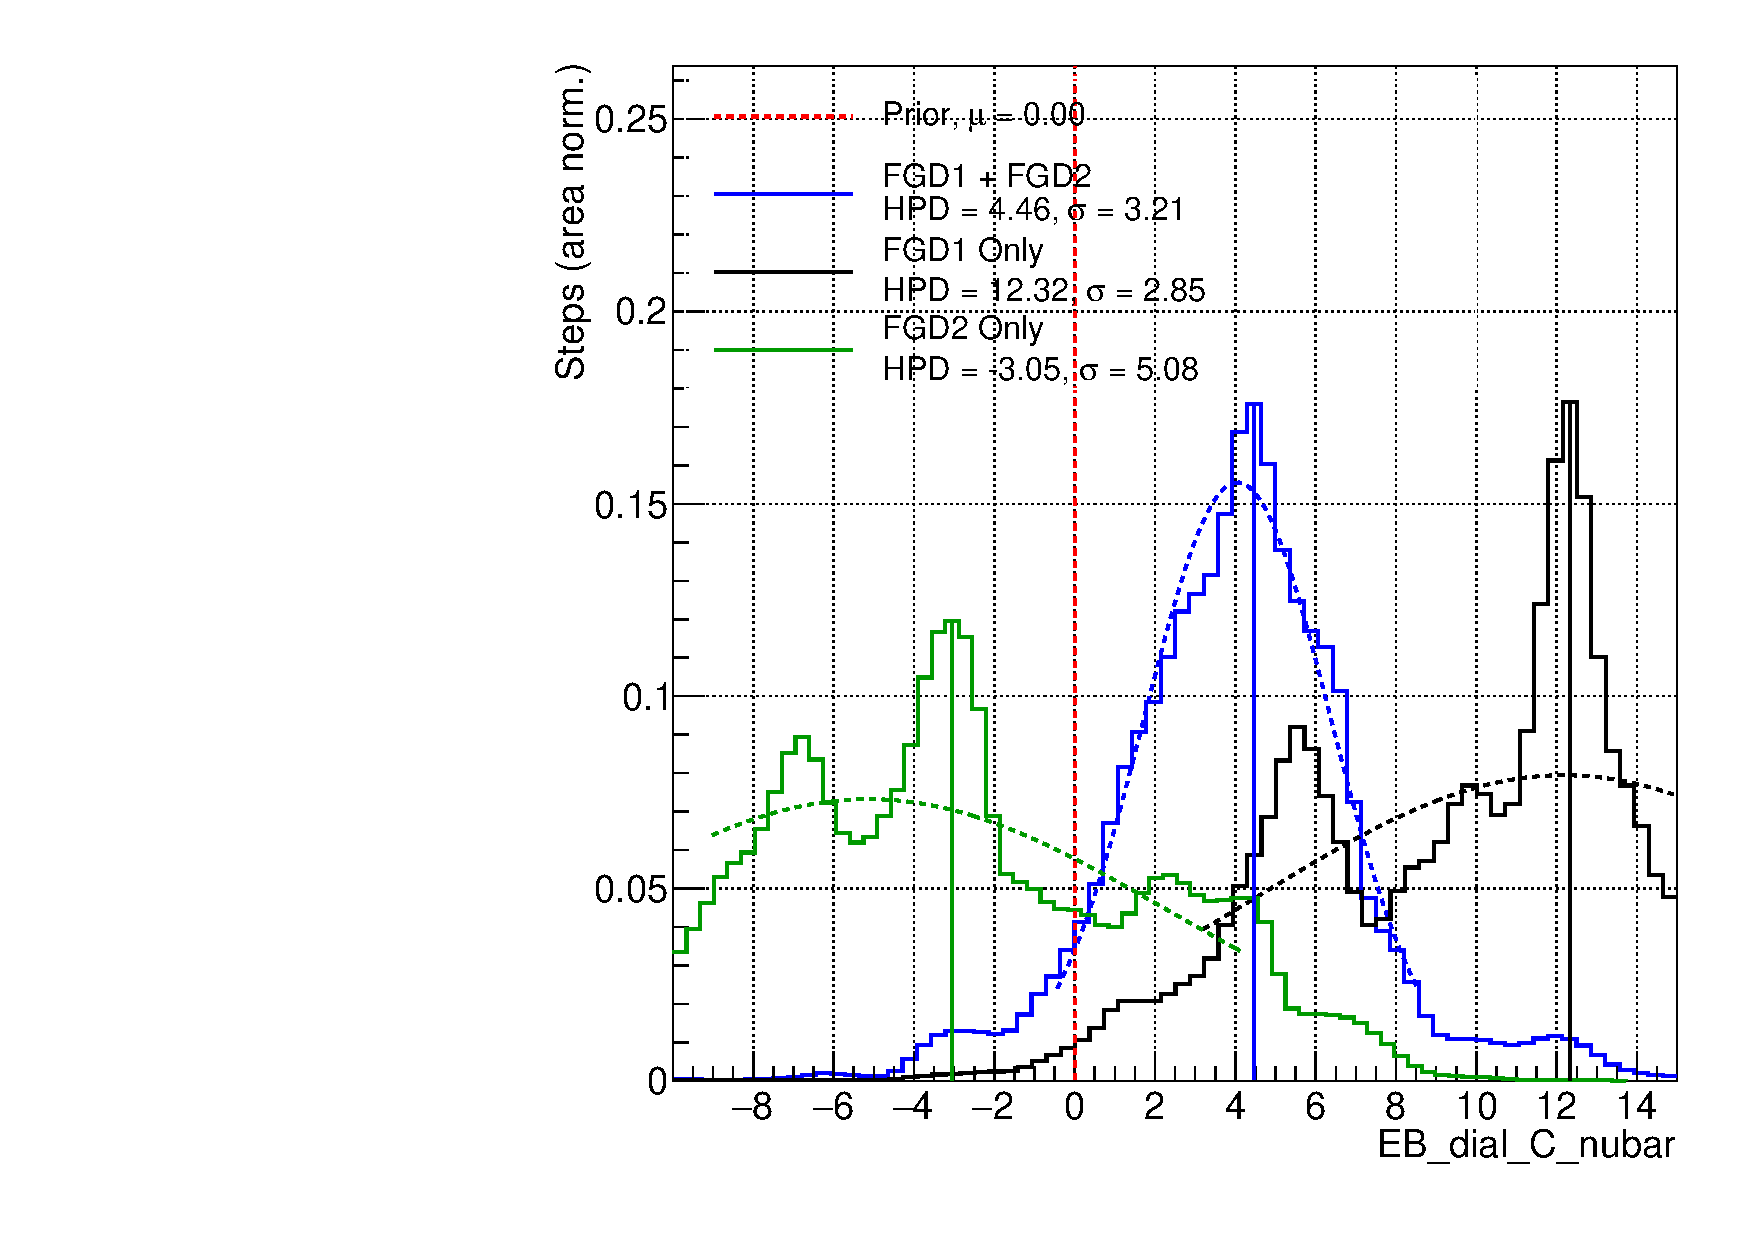
\includegraphics[width=0.73\linewidth]{figs/FGD_EB_dial_C_nubar}
  \caption{$E_{\mathrm{b}}\bar{\nu}$ C}
\end{subfigure} \\
\begin{subfigure}{.48\textwidth}
  \centering
  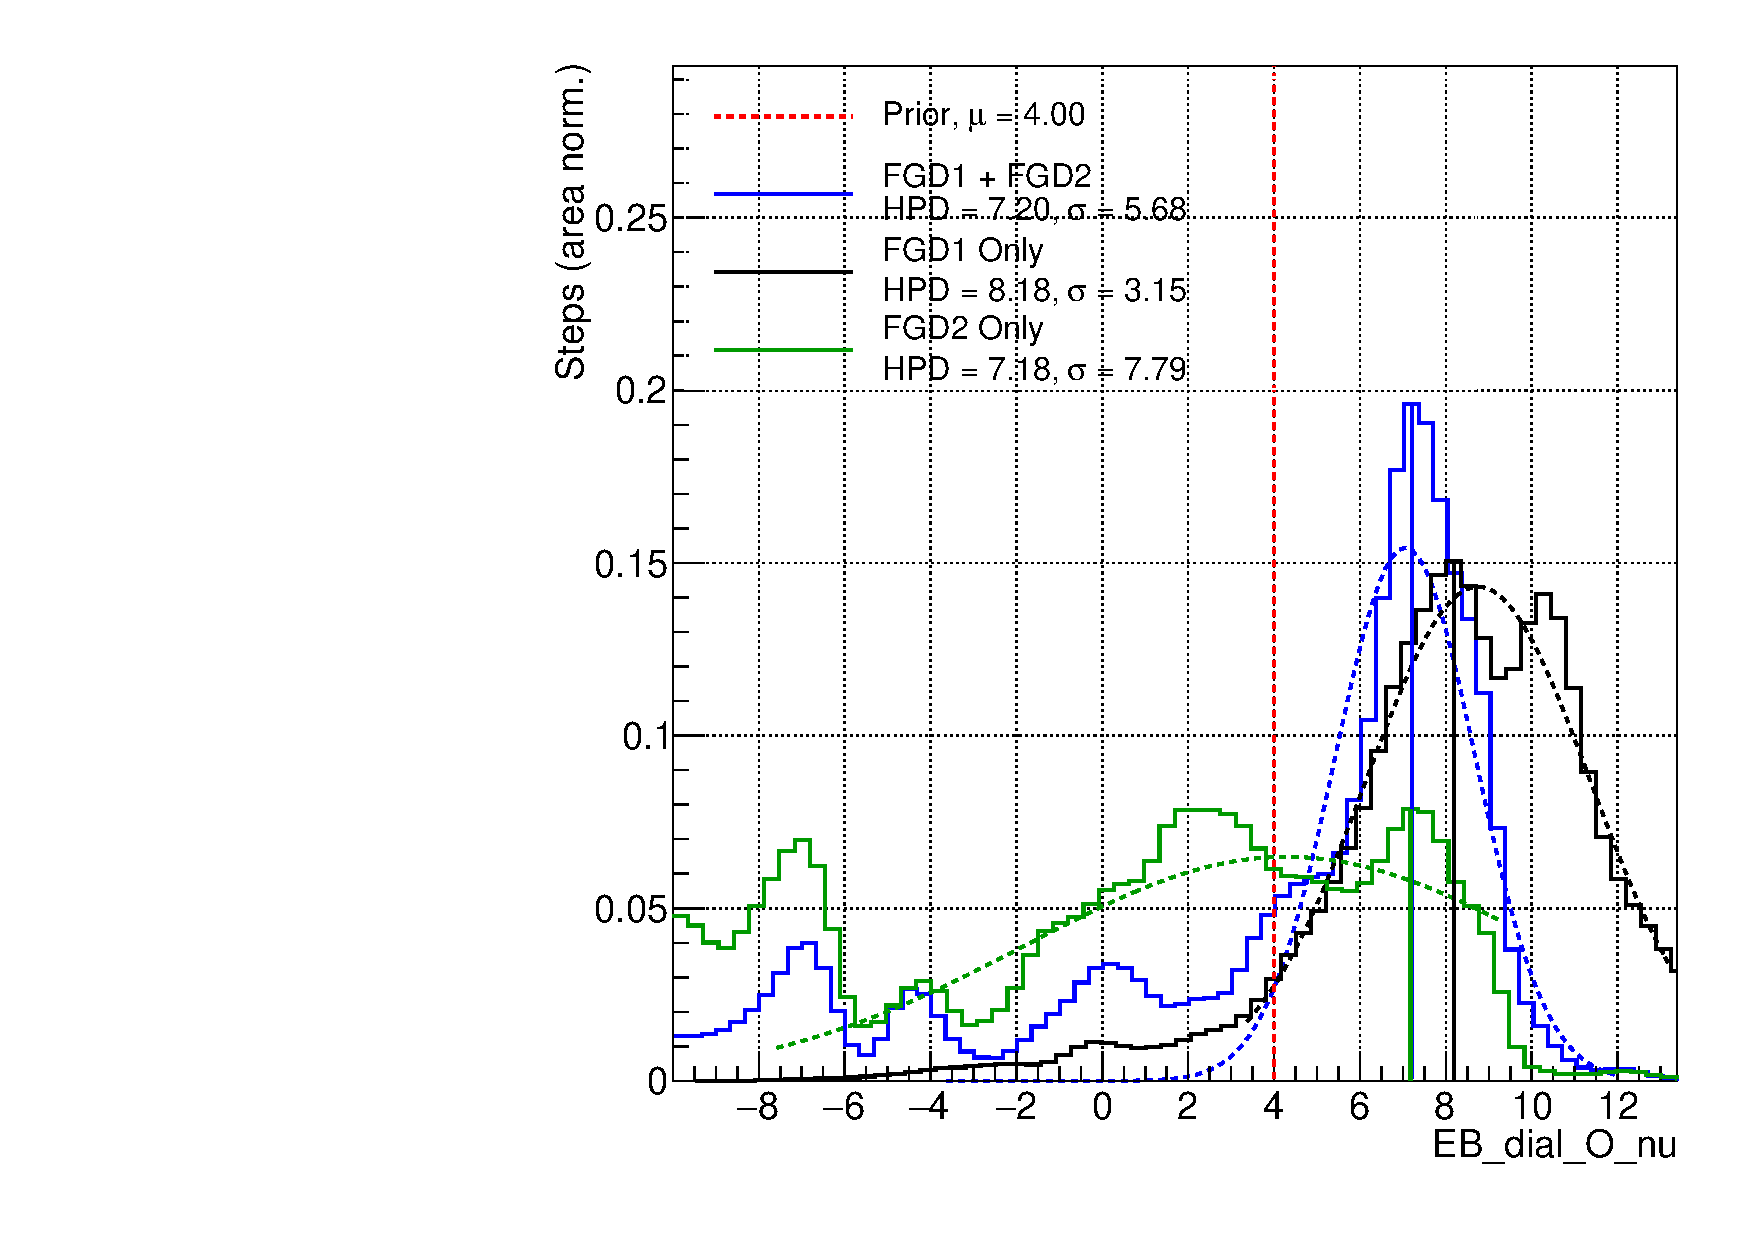
\includegraphics[width=0.73\linewidth]{figs/FGD_EB_dial_O_nu}
  \caption{$E_{\mathrm{b}}\nu$ O}
\end{subfigure}
\begin{subfigure}{.48\textwidth}
  \centering
  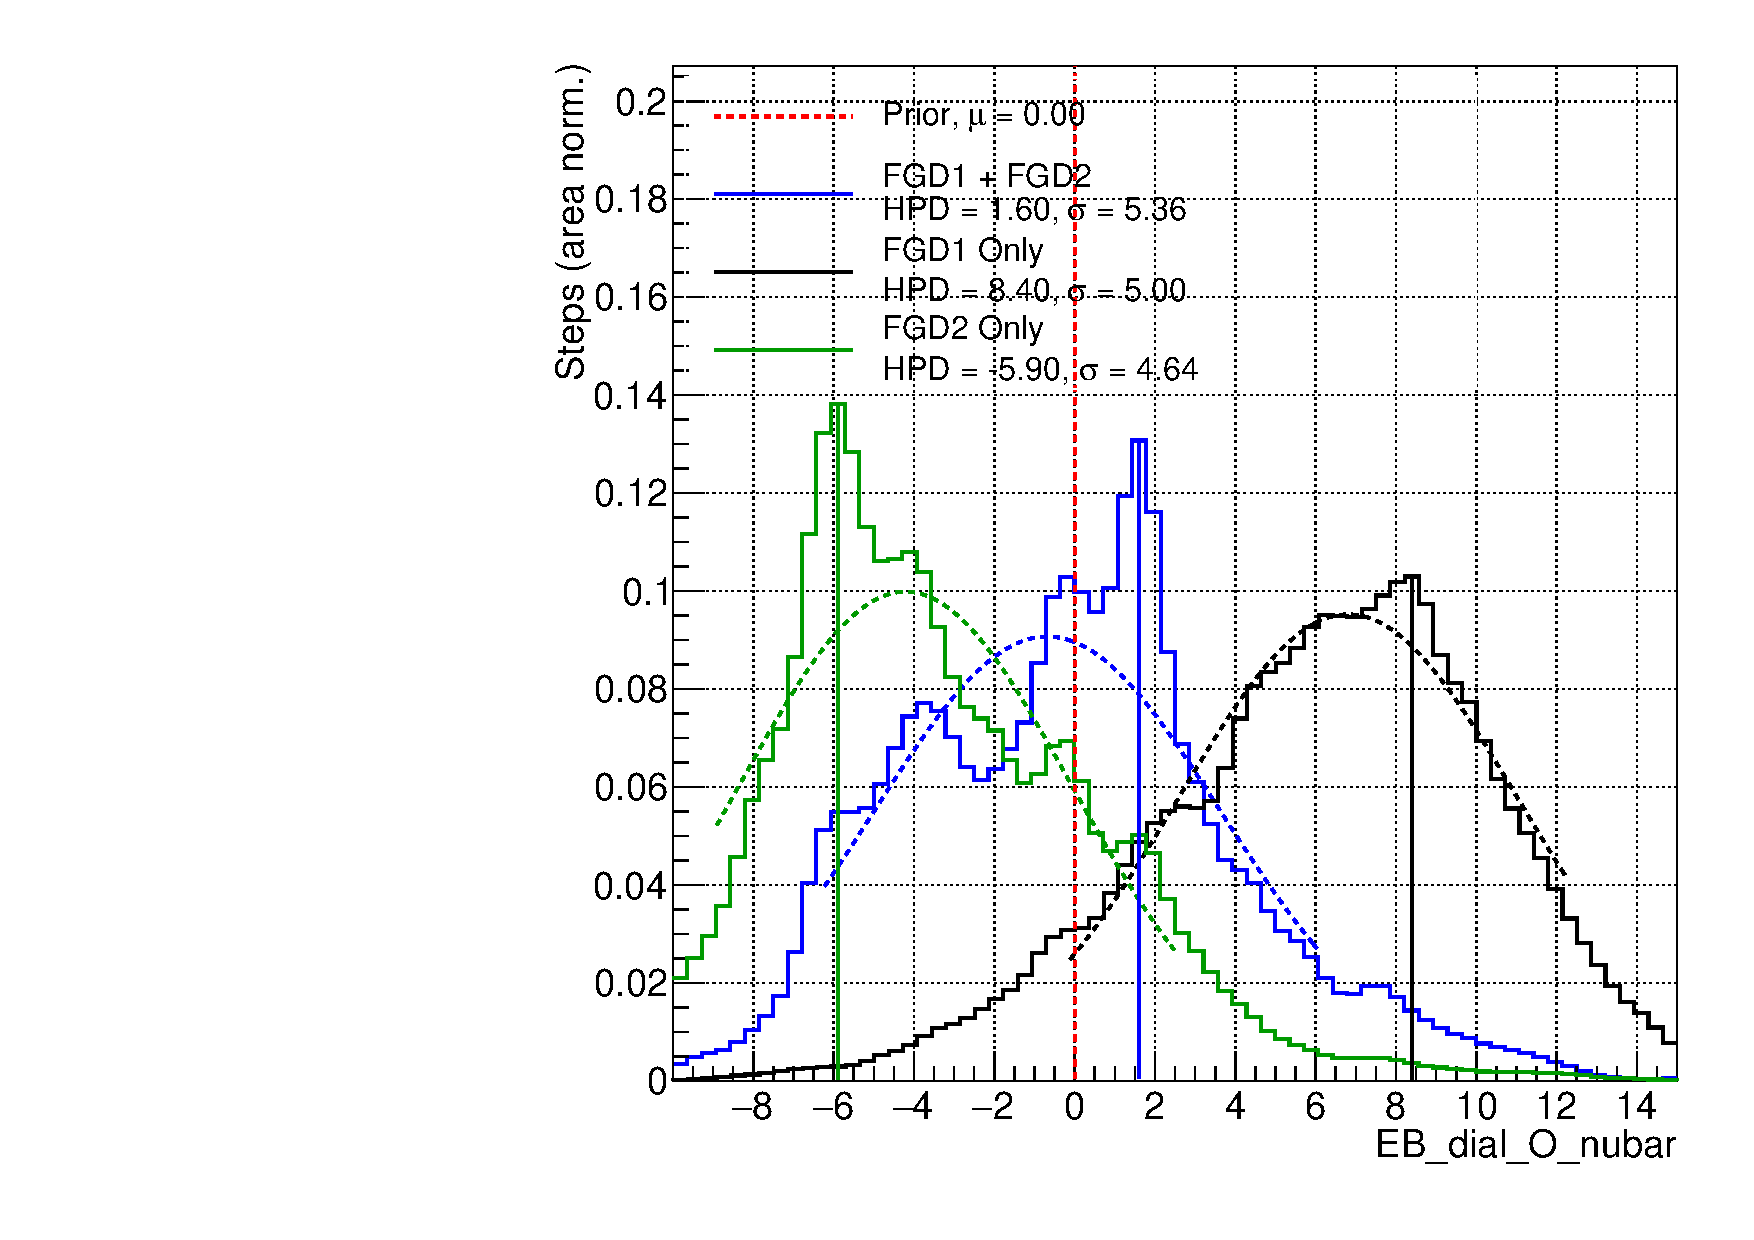
\includegraphics[width=0.73\linewidth]{figs/FGD_EB_dial_O_nubar}
  \caption{$E_{\mathrm{b}}\bar{\nu}$ O}
\end{subfigure}
\caption{Posterior distributions from the binding energy parameters for the FGD1 and FGD2 only fits.}
\label{fig:FGDEbdata}
\end{figure}

\section{FHC and RHC Only Fits}

For runs 2--4, 8, data was taken in FHC mode, and for runs 5--7, 9, data was taken in RHC mode. To see the compatibility of the model fit to neutrino and anti-neutrino data, fits were running using runs 2--4+8 and runs 5--7+9 separately. As the amount of FHC data is $\sim$3$\times$ larger than for RHC, it is expected there will be larger constraints for the FHC only fit.

The results for the flux parameters are shown in Figures \ref{fig:fhcrhcfluxND} and \ref{fig:fhcrhcfluxSK}. The shape of the pulls are very similar for the three fits, but for RHC only the parameters are consistently closer to nominal than for FHC only, with the full fit value lying between the two. In the FHC fit, the RHC flux parameters are constrained via the prior correlations with the FHC flux parameters, and vice versa.

\begin{figure}
\centering
\begin{subfigure}{0.3\textwidth}
  \centering
  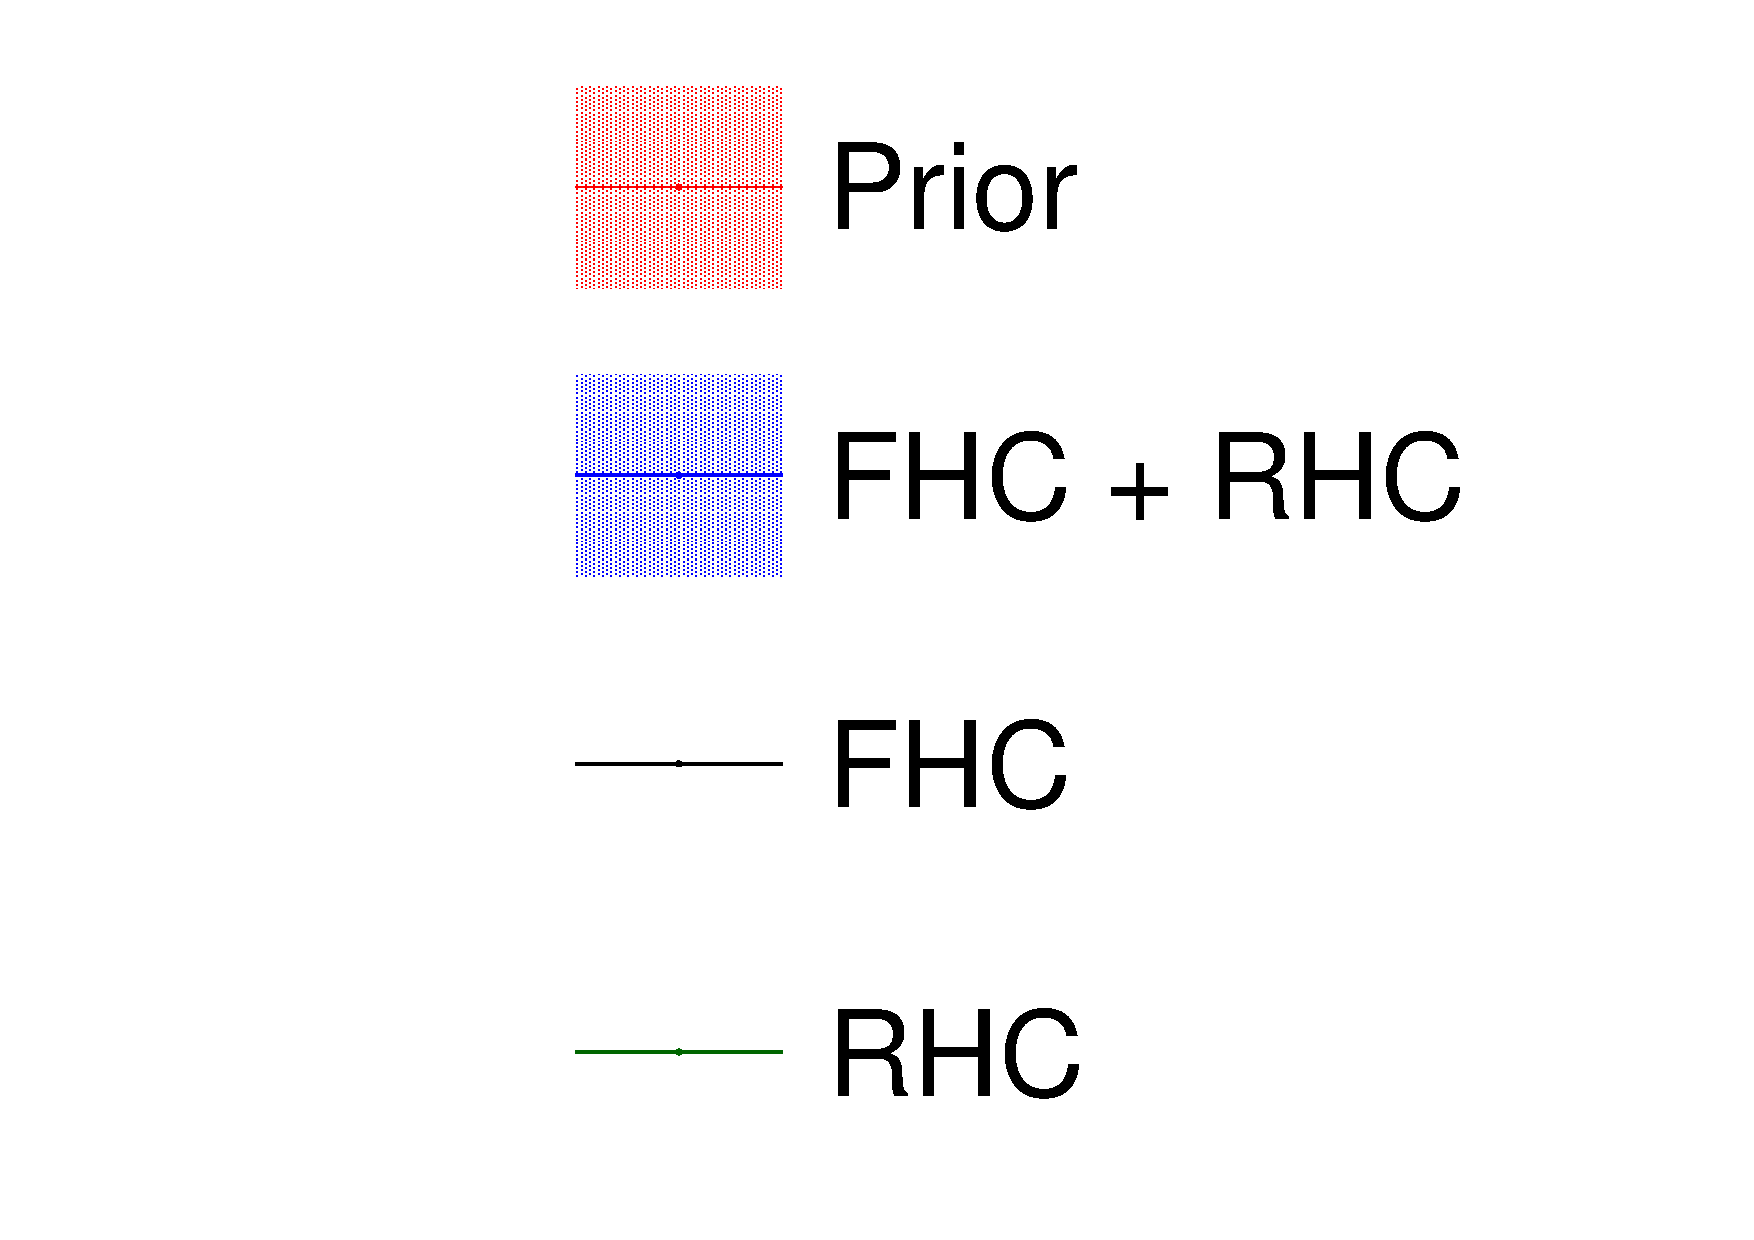
\includegraphics[width=1.0\linewidth, trim={5mm  90mm 0mm 0mm}, clip]{figs/fhcrhcfits_leg}
\end{subfigure}
\begin{subfigure}{0.3\textwidth}
  \centering
  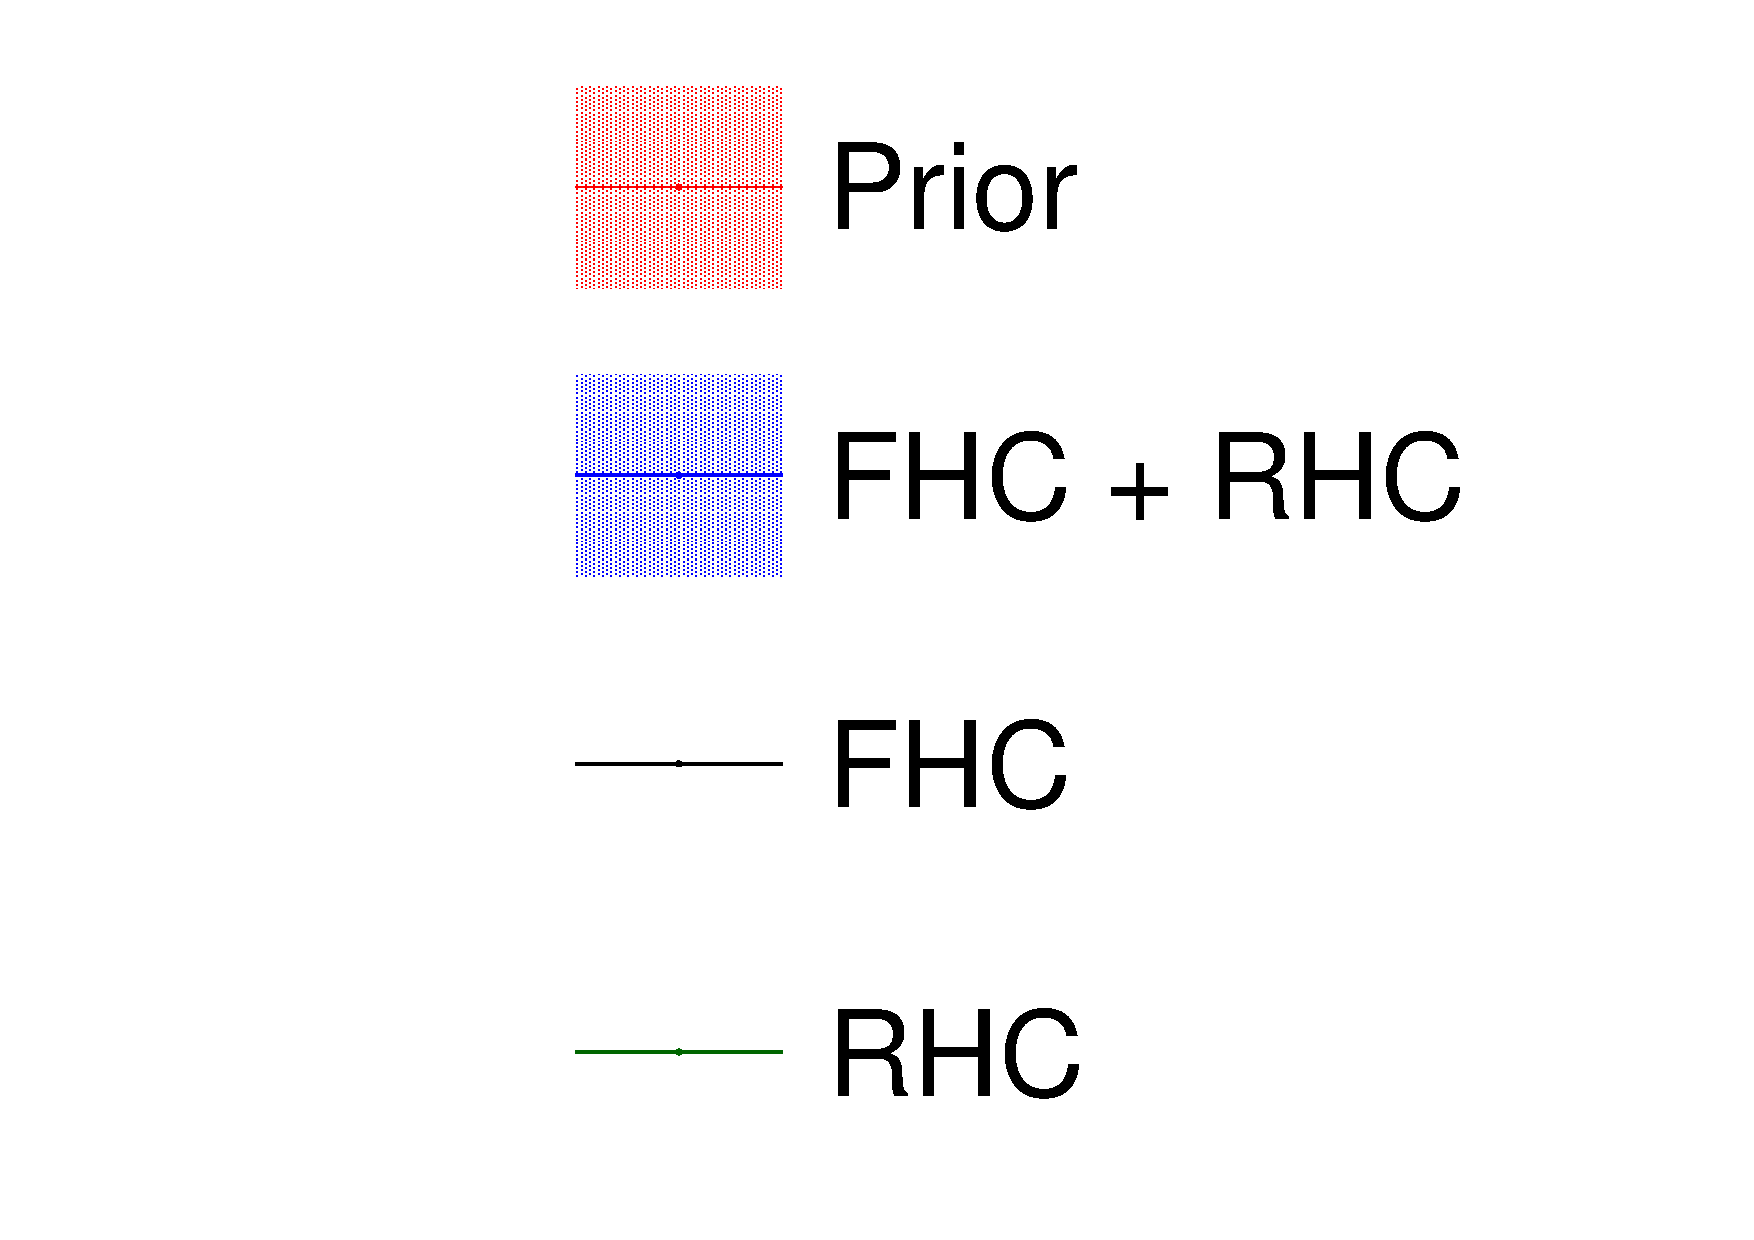
\includegraphics[width=1.0\linewidth, trim={5mm  0mm 0mm 95mm}, clip]{figs/fhcrhcfits_leg}
\end{subfigure}
\begin{subfigure}{0.45\textwidth}
  \centering
  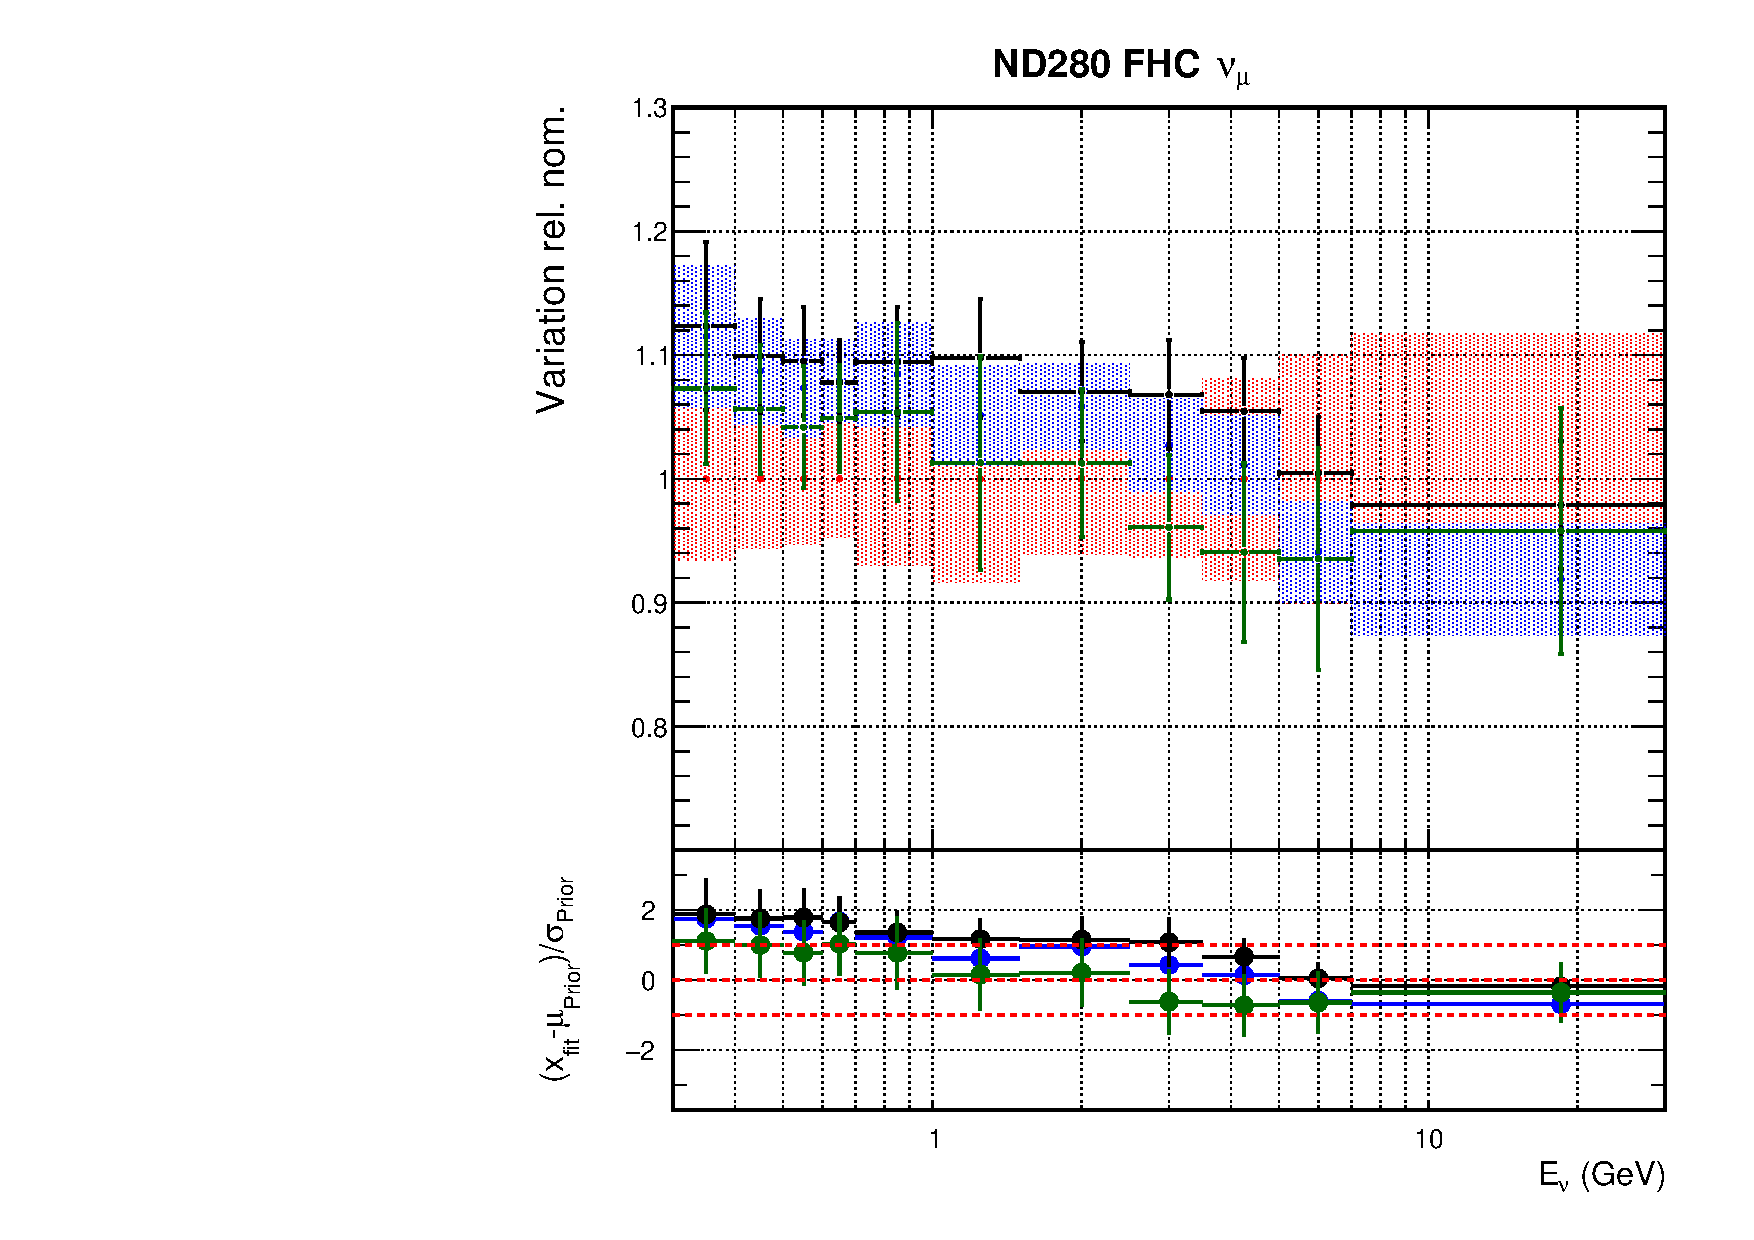
\includegraphics[width=0.75\linewidth]{figs/fhcrhcfitsflux_0}
  \caption{ND FHC $\nu_{\mu}$}
\end{subfigure}
\begin{subfigure}{0.45\textwidth}
  \centering
  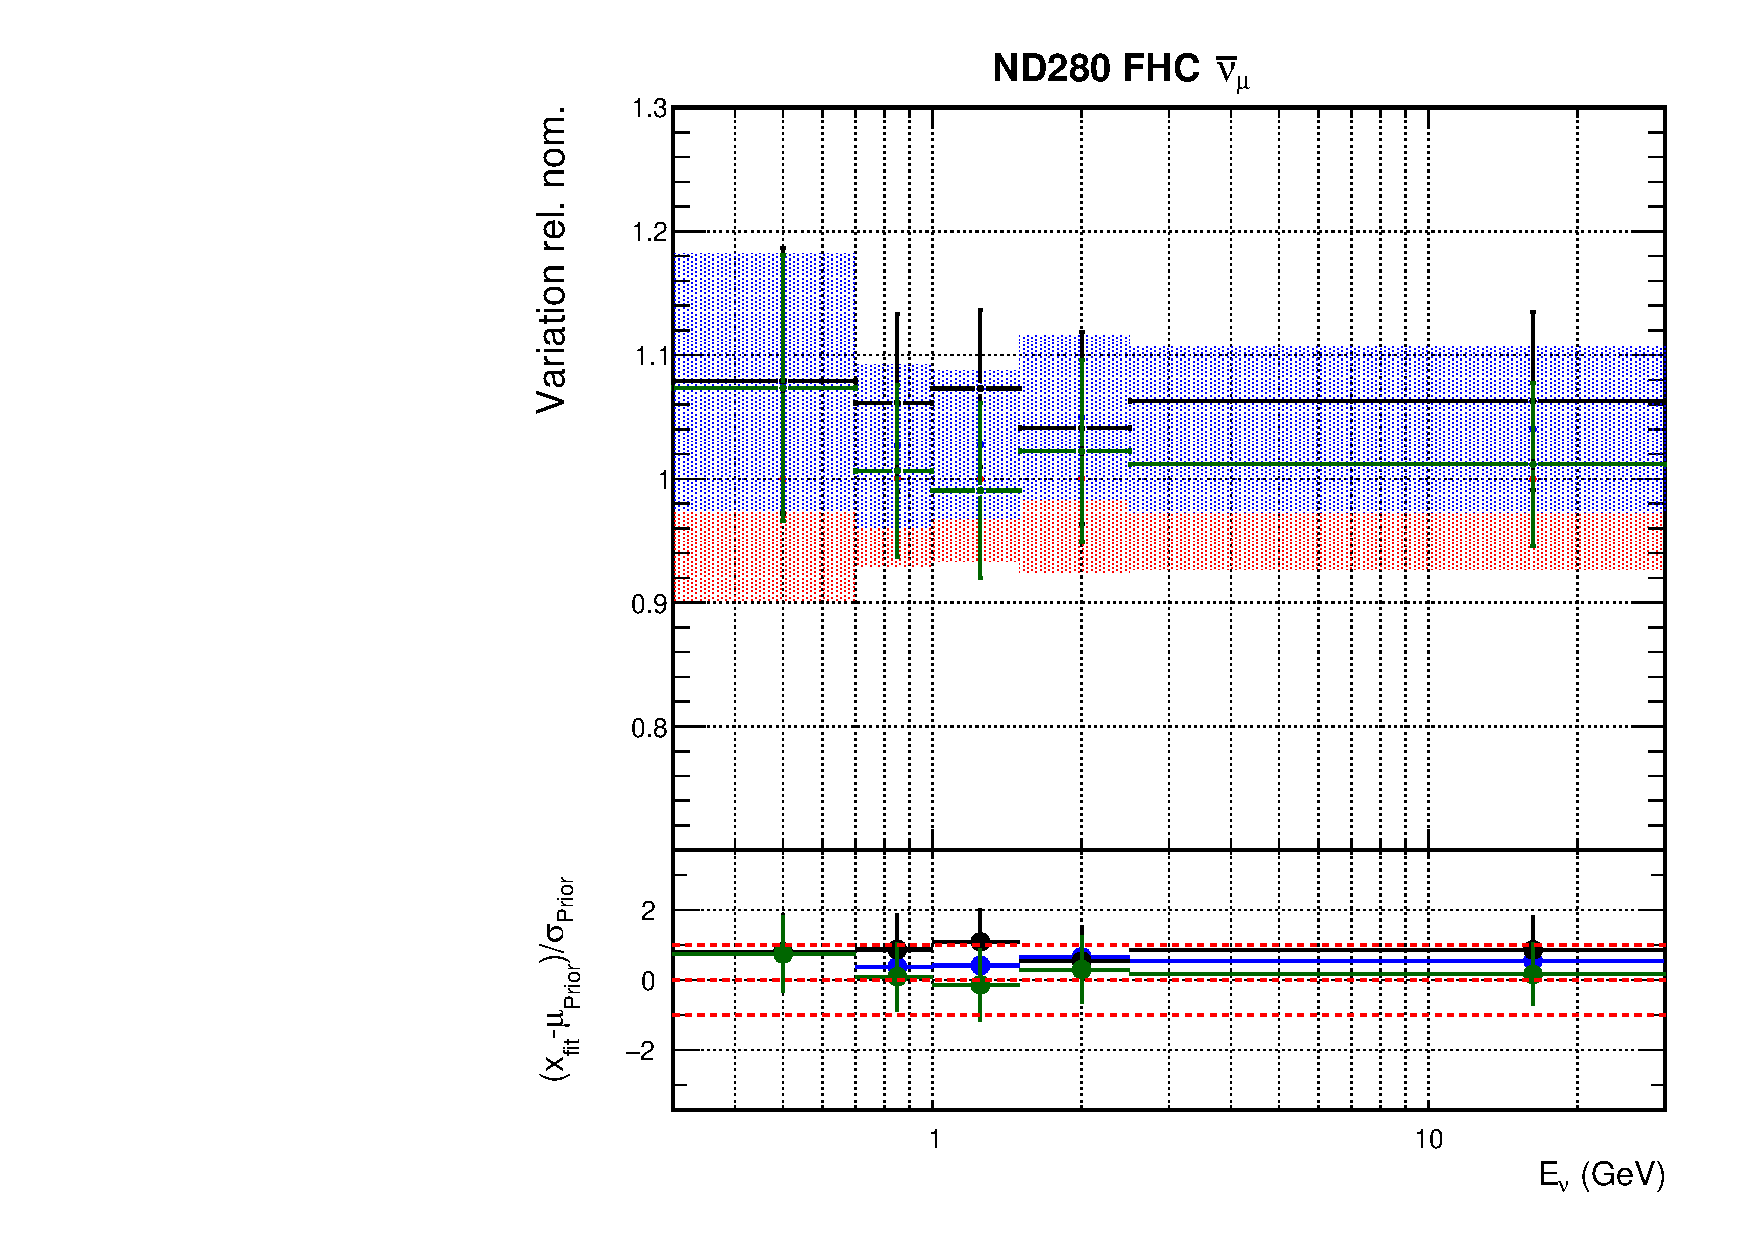
\includegraphics[width=0.75\linewidth]{figs/fhcrhcfitsflux_1}
  \caption{ND FHC $\bar{\nu_{\mu}}$}
\end{subfigure}
\begin{subfigure}{0.45\textwidth}
  \centering
  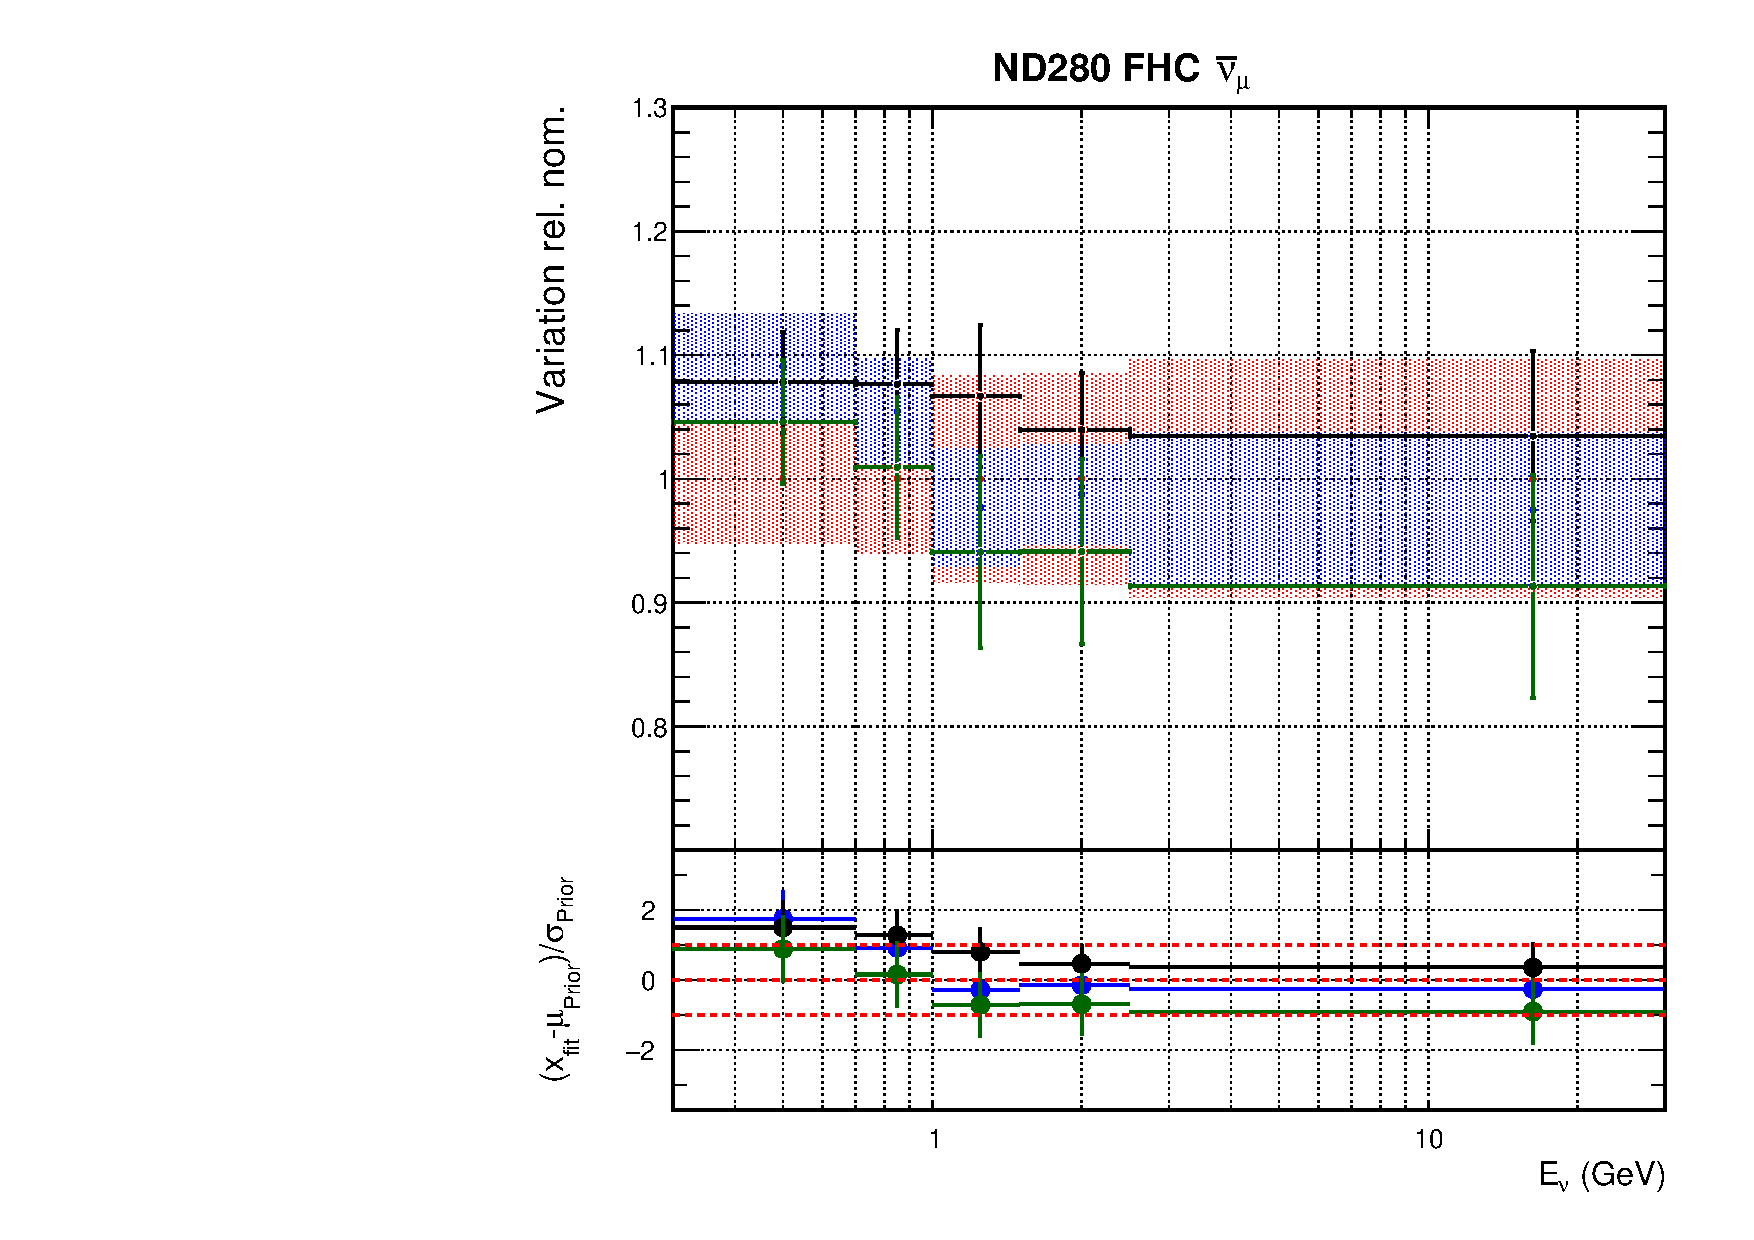
\includegraphics[width=0.75\linewidth]{figs/fhcrhcfitsflux_2}
  \caption{ND FHC $\nu_e$}
\end{subfigure}
\begin{subfigure}{0.45\textwidth}
  \centering
  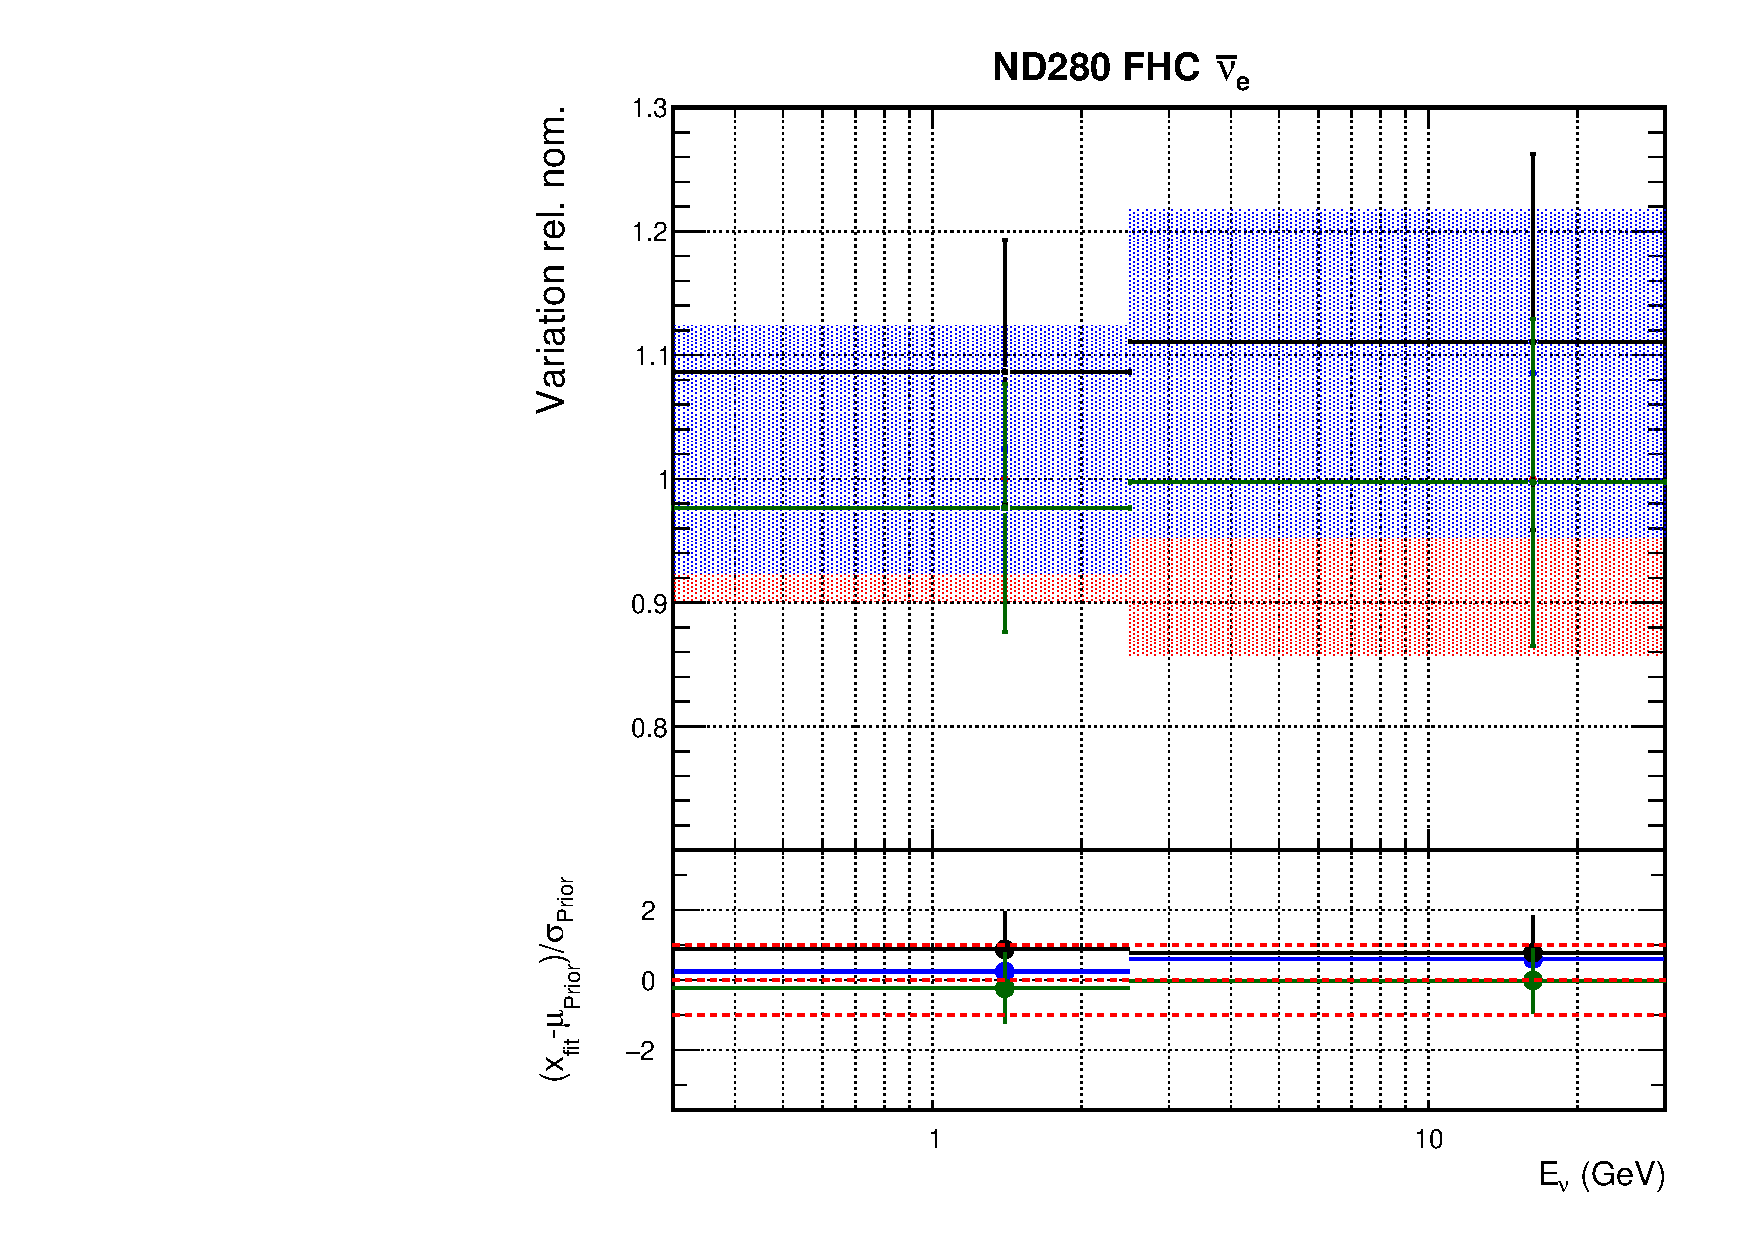
\includegraphics[width=0.75\linewidth]{figs/fhcrhcfitsflux_3}
  \caption{ND FHC $\bar{\nu_{e}}$}
\end{subfigure}
\begin{subfigure}{0.45\textwidth}
  \centering
  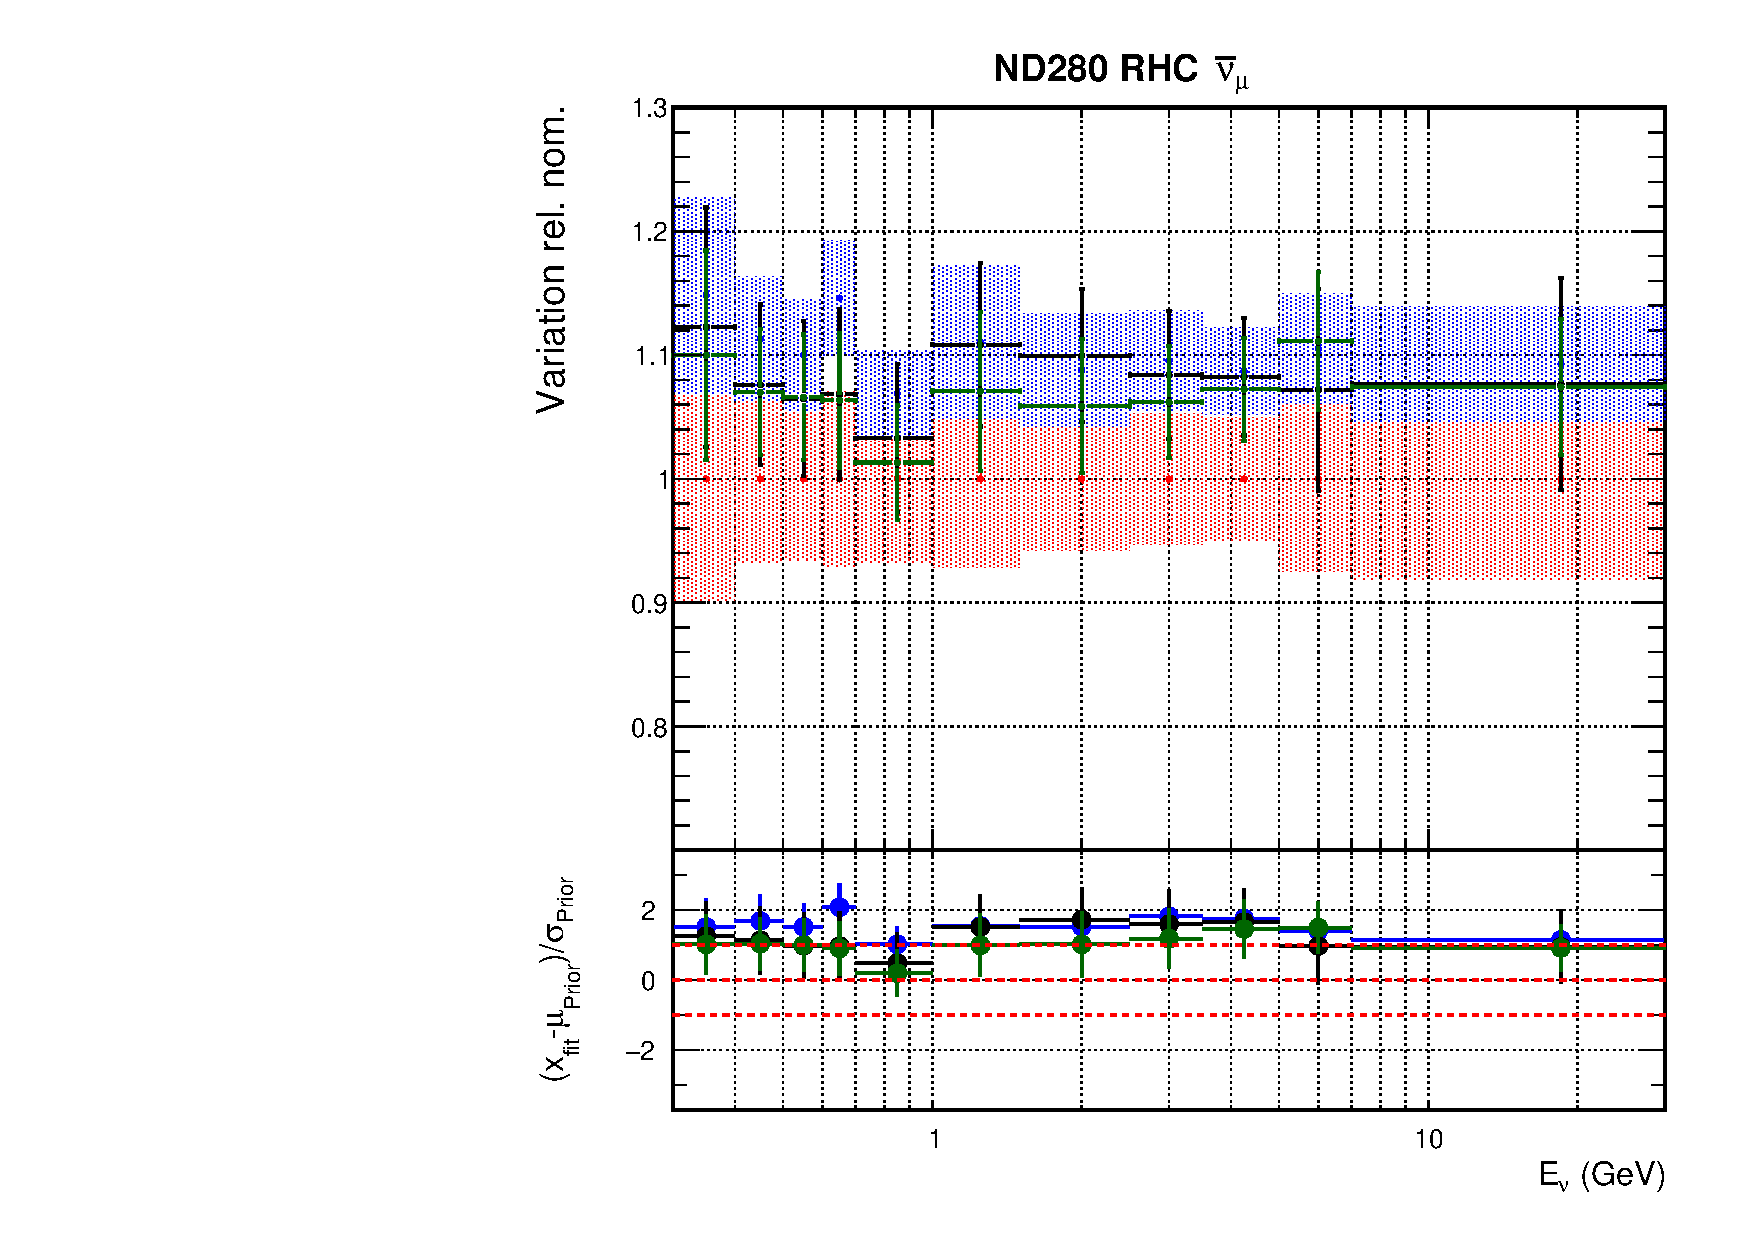
\includegraphics[width=0.75\linewidth]{figs/fhcrhcfitsflux_4}
  \caption{ND RHC $\nu_{\mu}$}
\end{subfigure}
\begin{subfigure}{0.45\textwidth}
  \centering
  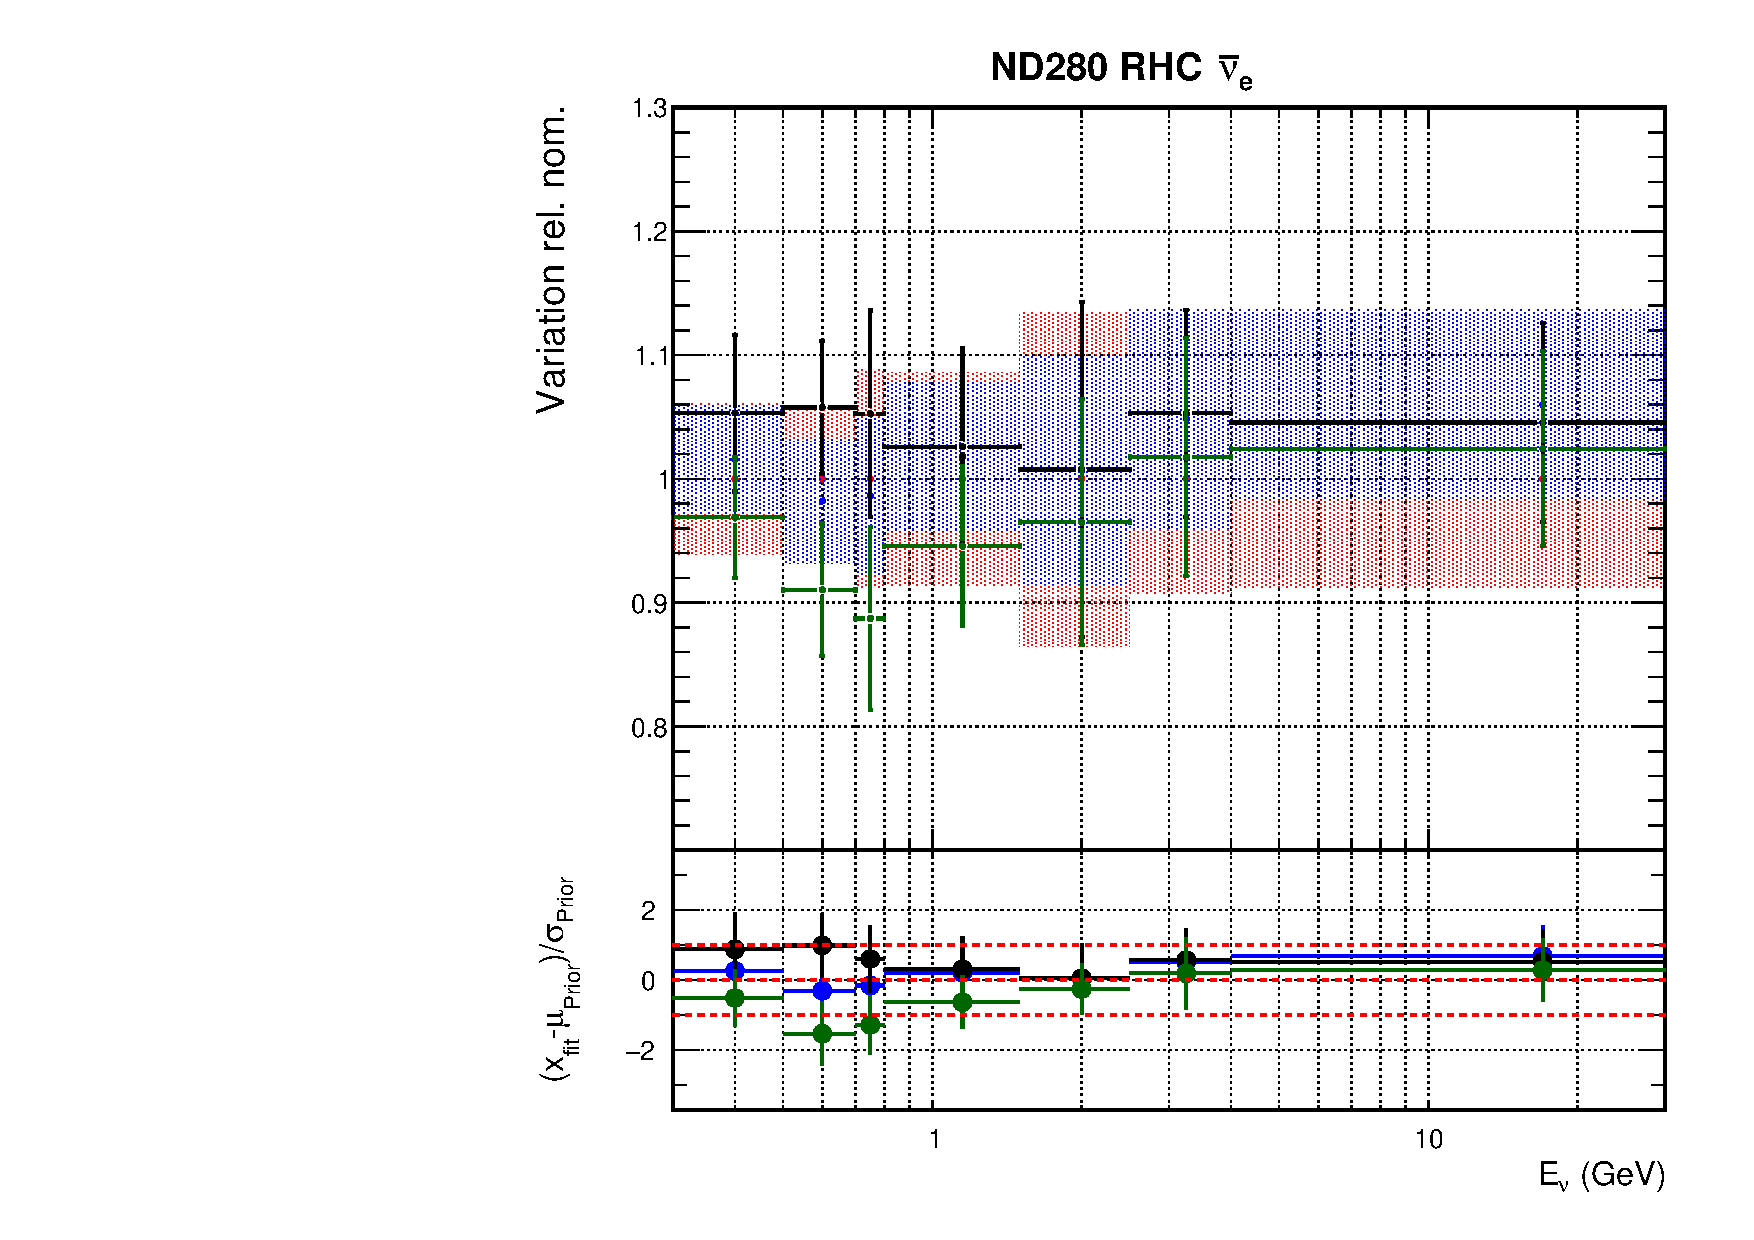
\includegraphics[width=0.75\linewidth]{figs/fhcrhcfitsflux_5}
  \caption{ND RHC $\bar{\nu_{\mu}}$}
\end{subfigure}
\begin{subfigure}{0.45\textwidth}
  \centering
  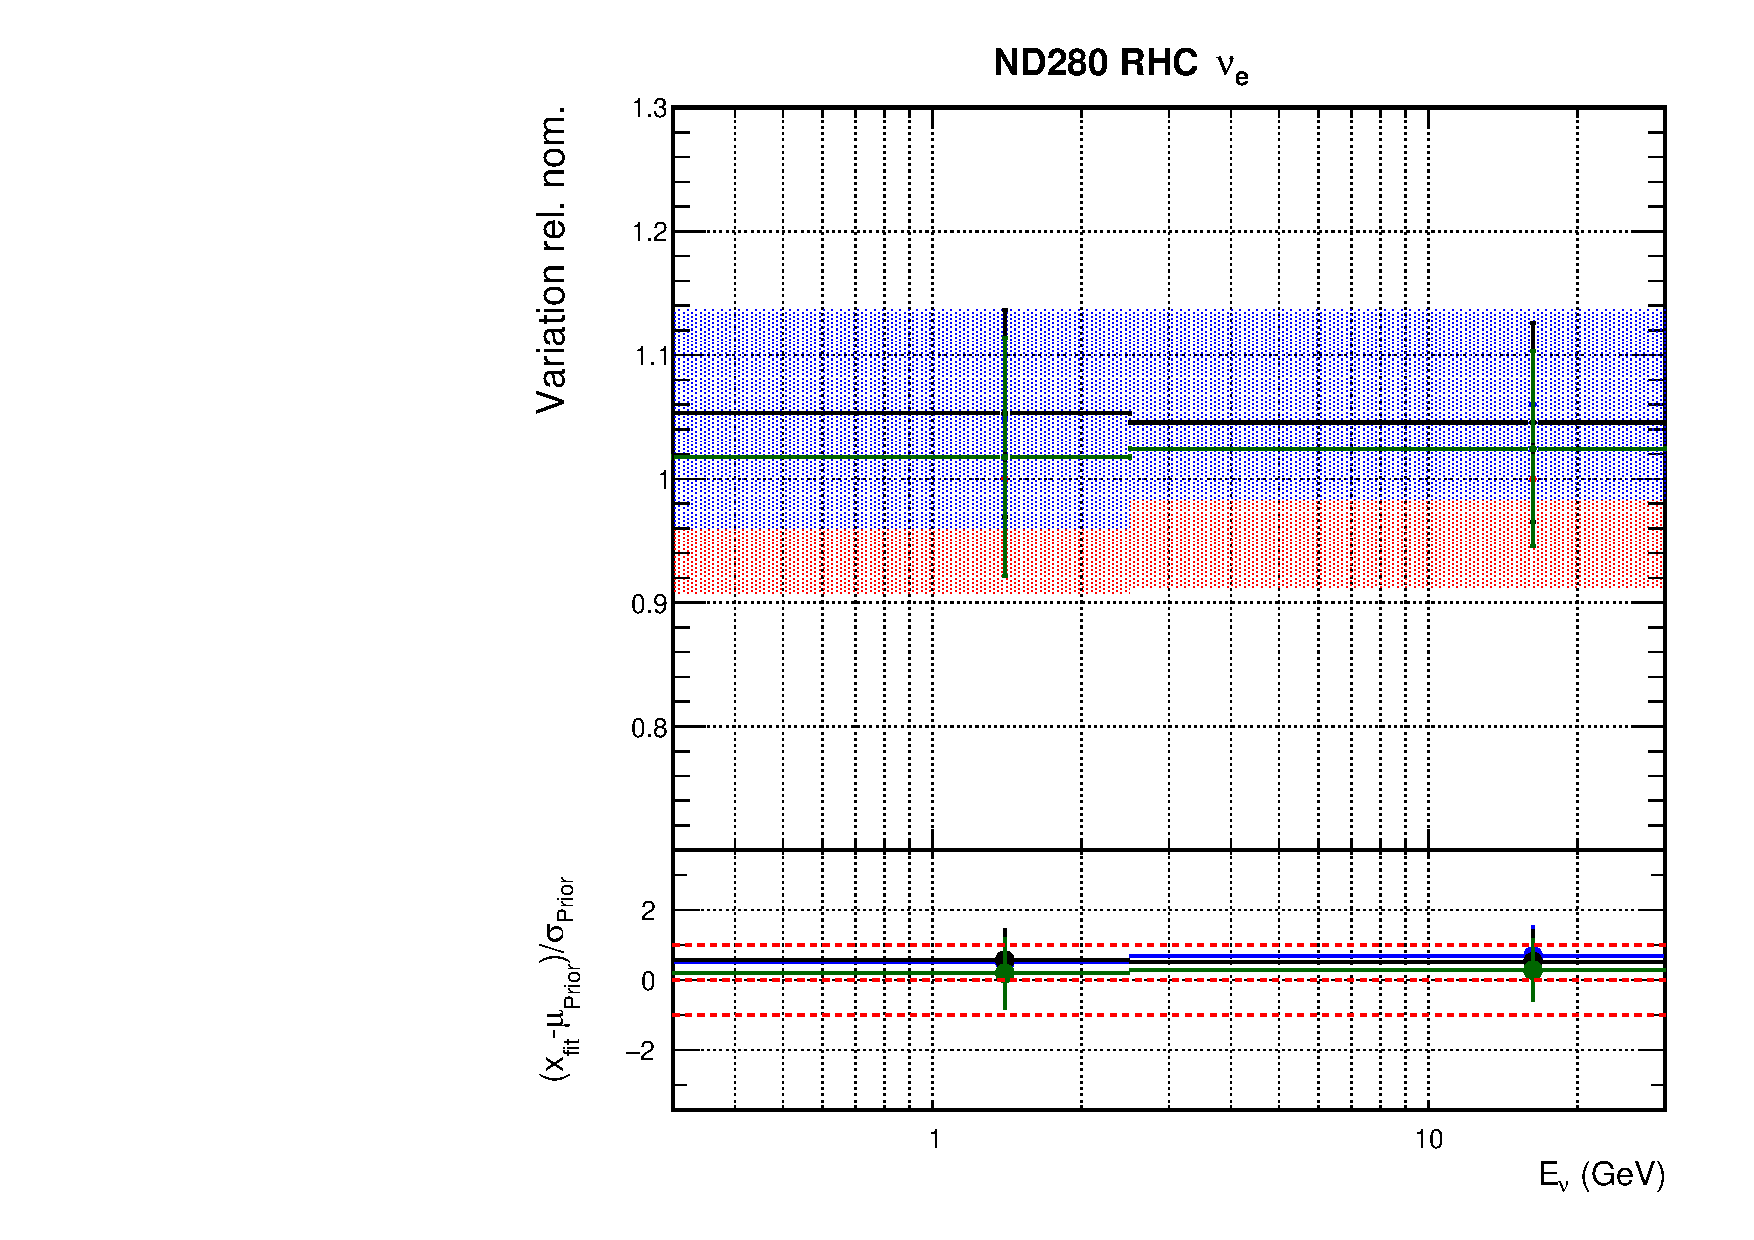
\includegraphics[width=0.75\linewidth]{figs/fhcrhcfitsflux_6}
  \caption{ND RHC $\nu_e$}
\end{subfigure}
\begin{subfigure}{0.45\textwidth}
  \centering
  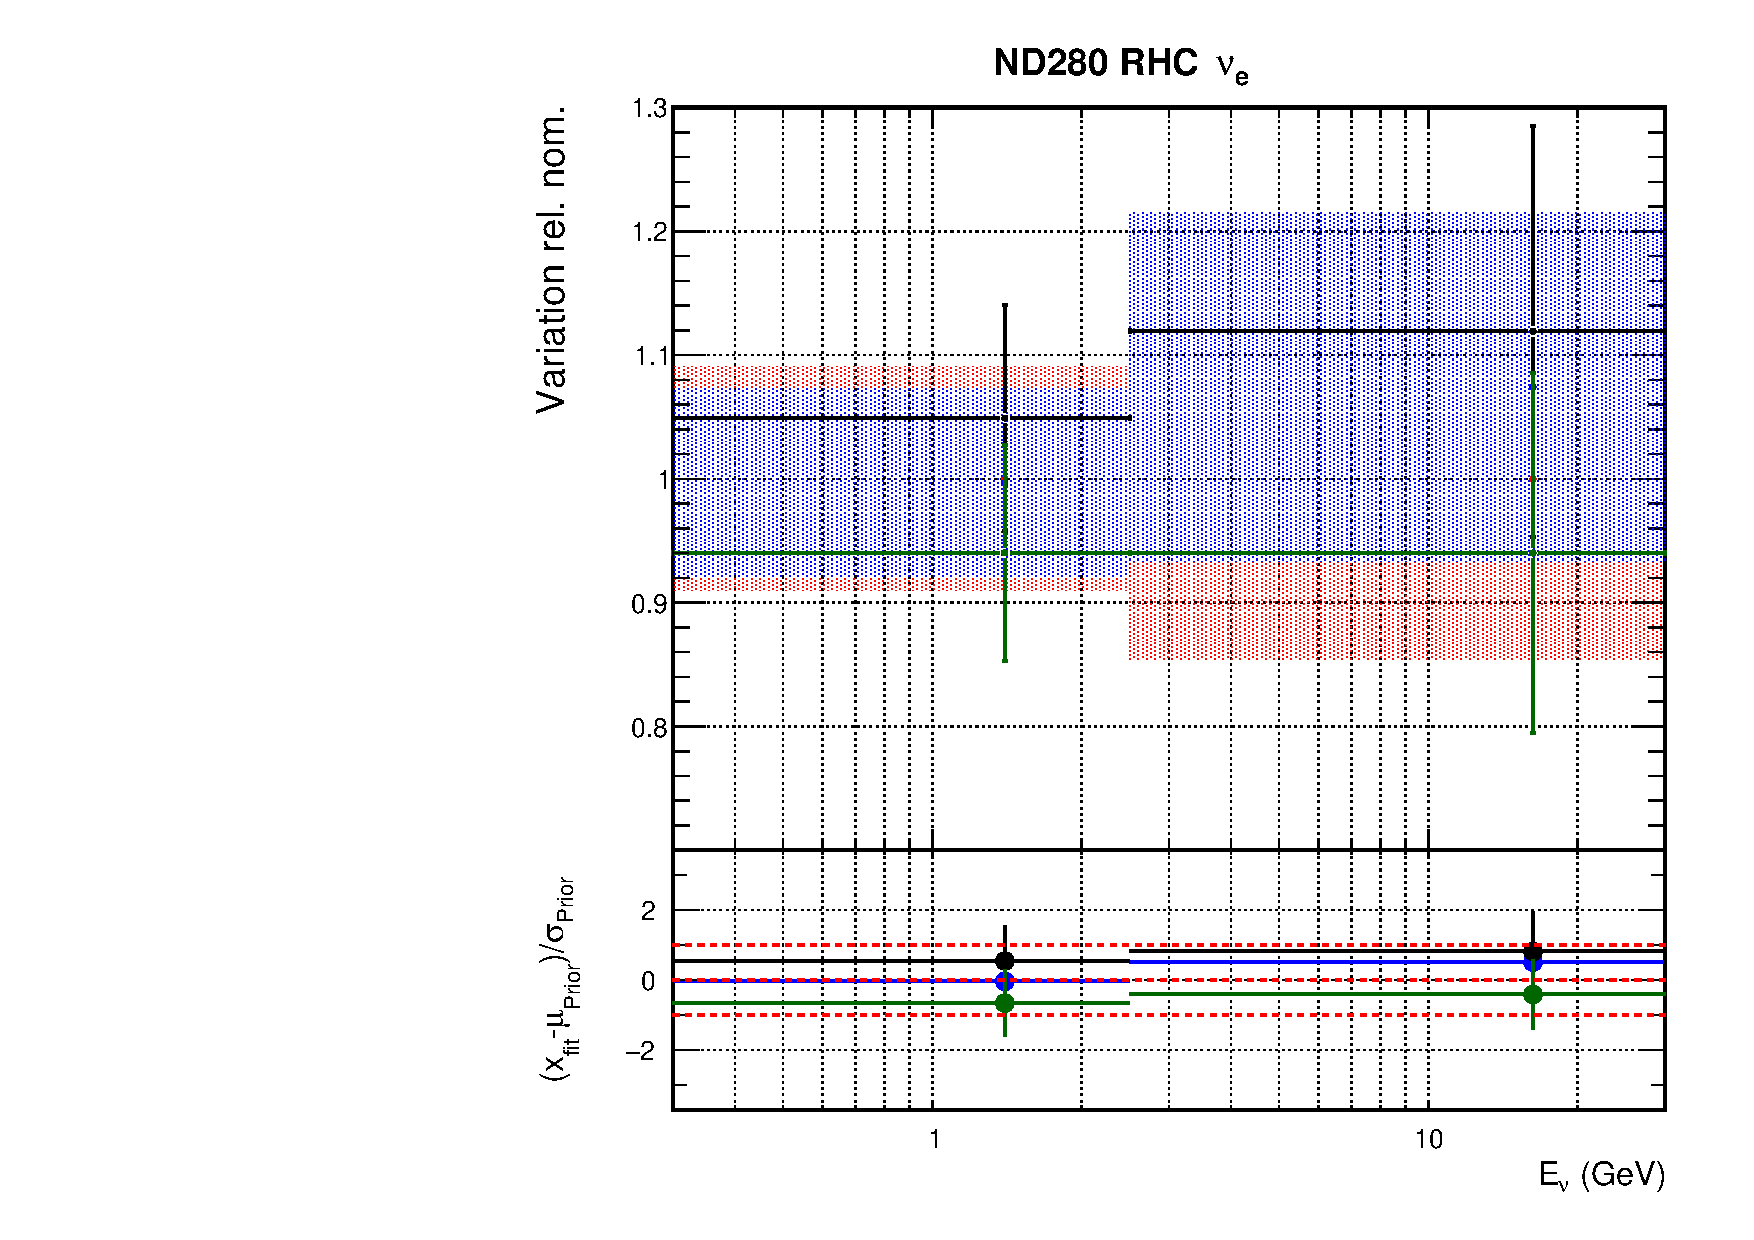
\includegraphics[width=0.75\linewidth]{figs/fhcrhcfitsflux_7}
  \caption{ND RHC $\bar{\nu_e}$}
\end{subfigure}
\caption{ND flux parameters for the FHC and RHC only fits.}
\label{fig:fhcrhcfluxND}
\end{figure}

\begin{figure}
\centering
\begin{subfigure}{0.3\textwidth}
  \centering
  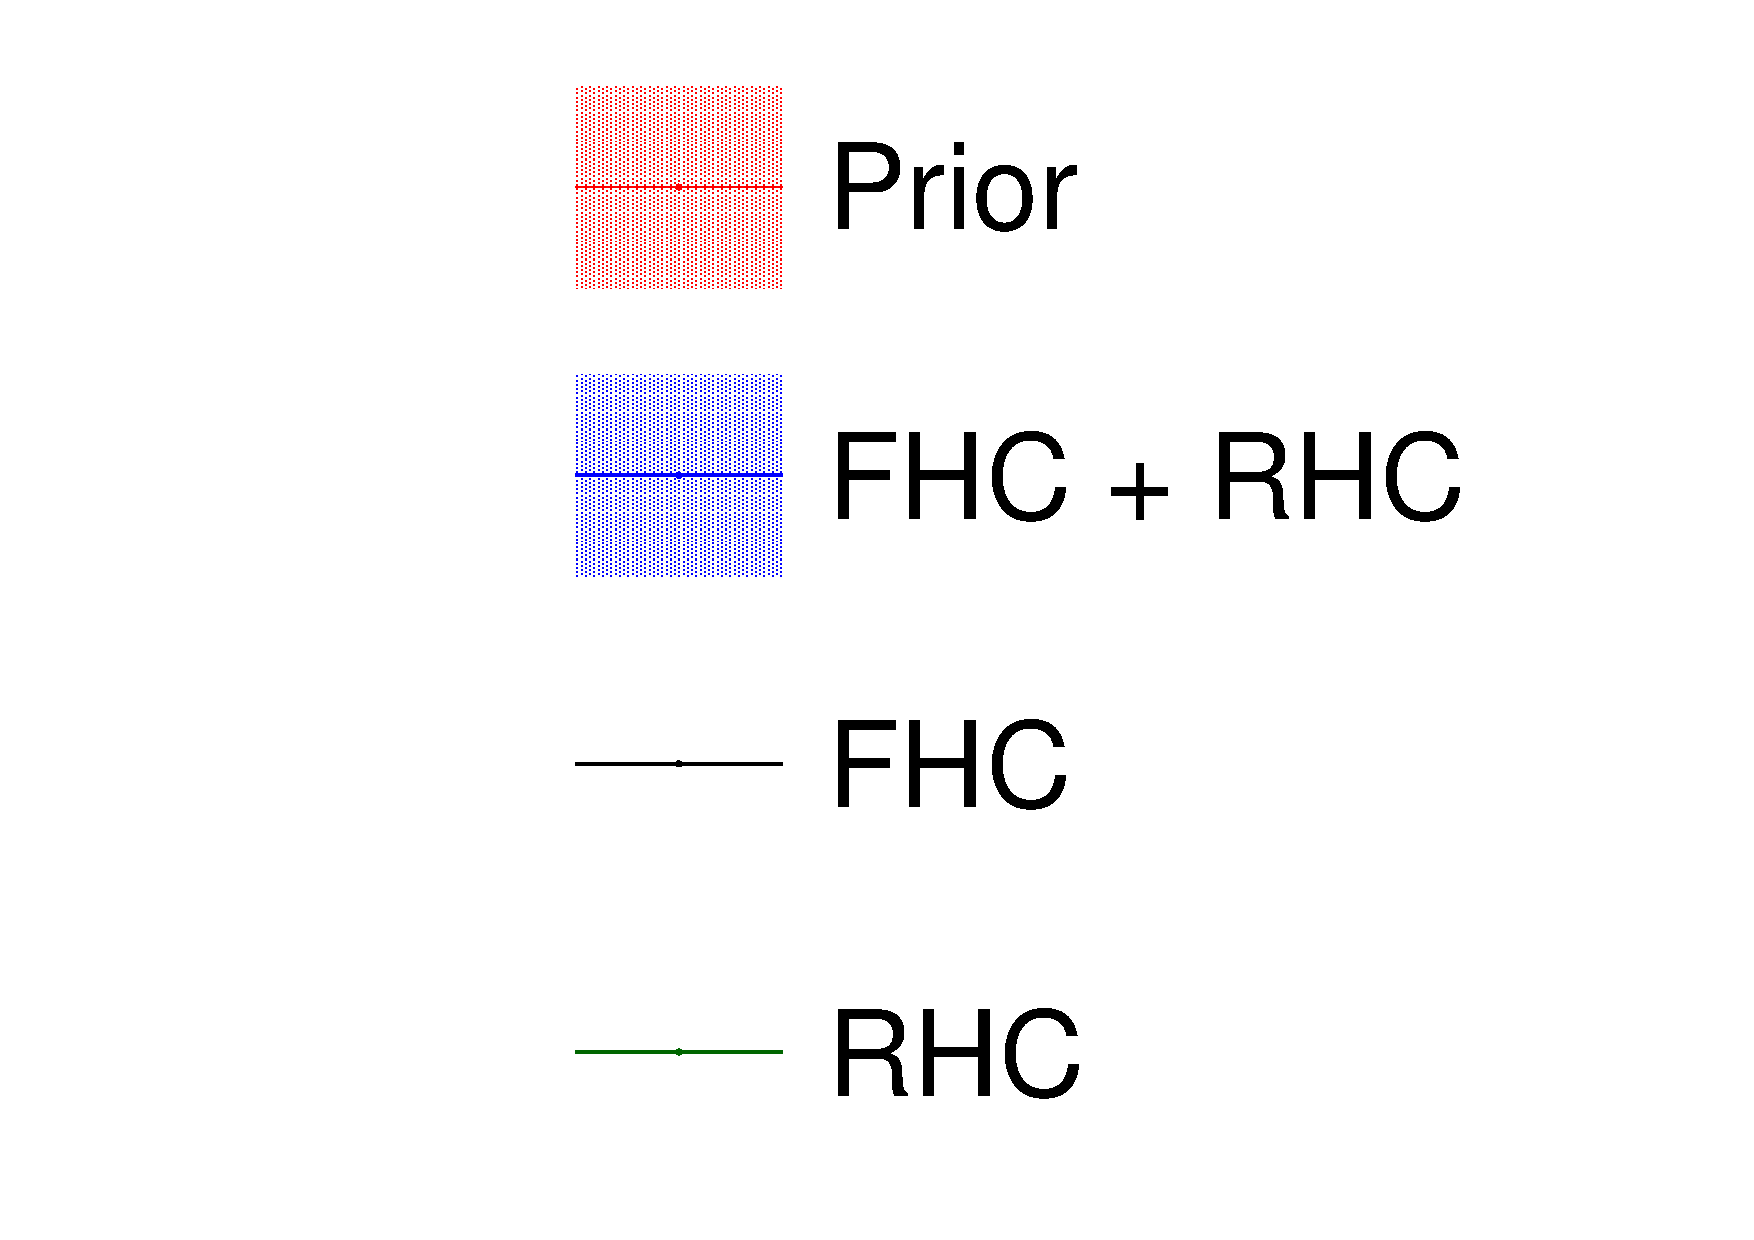
\includegraphics[width=1.0\linewidth, trim={5mm  90mm 0mm 0mm}, clip]{figs/fhcrhcfits_leg}
\end{subfigure}
\begin{subfigure}{0.3\textwidth}
  \centering
  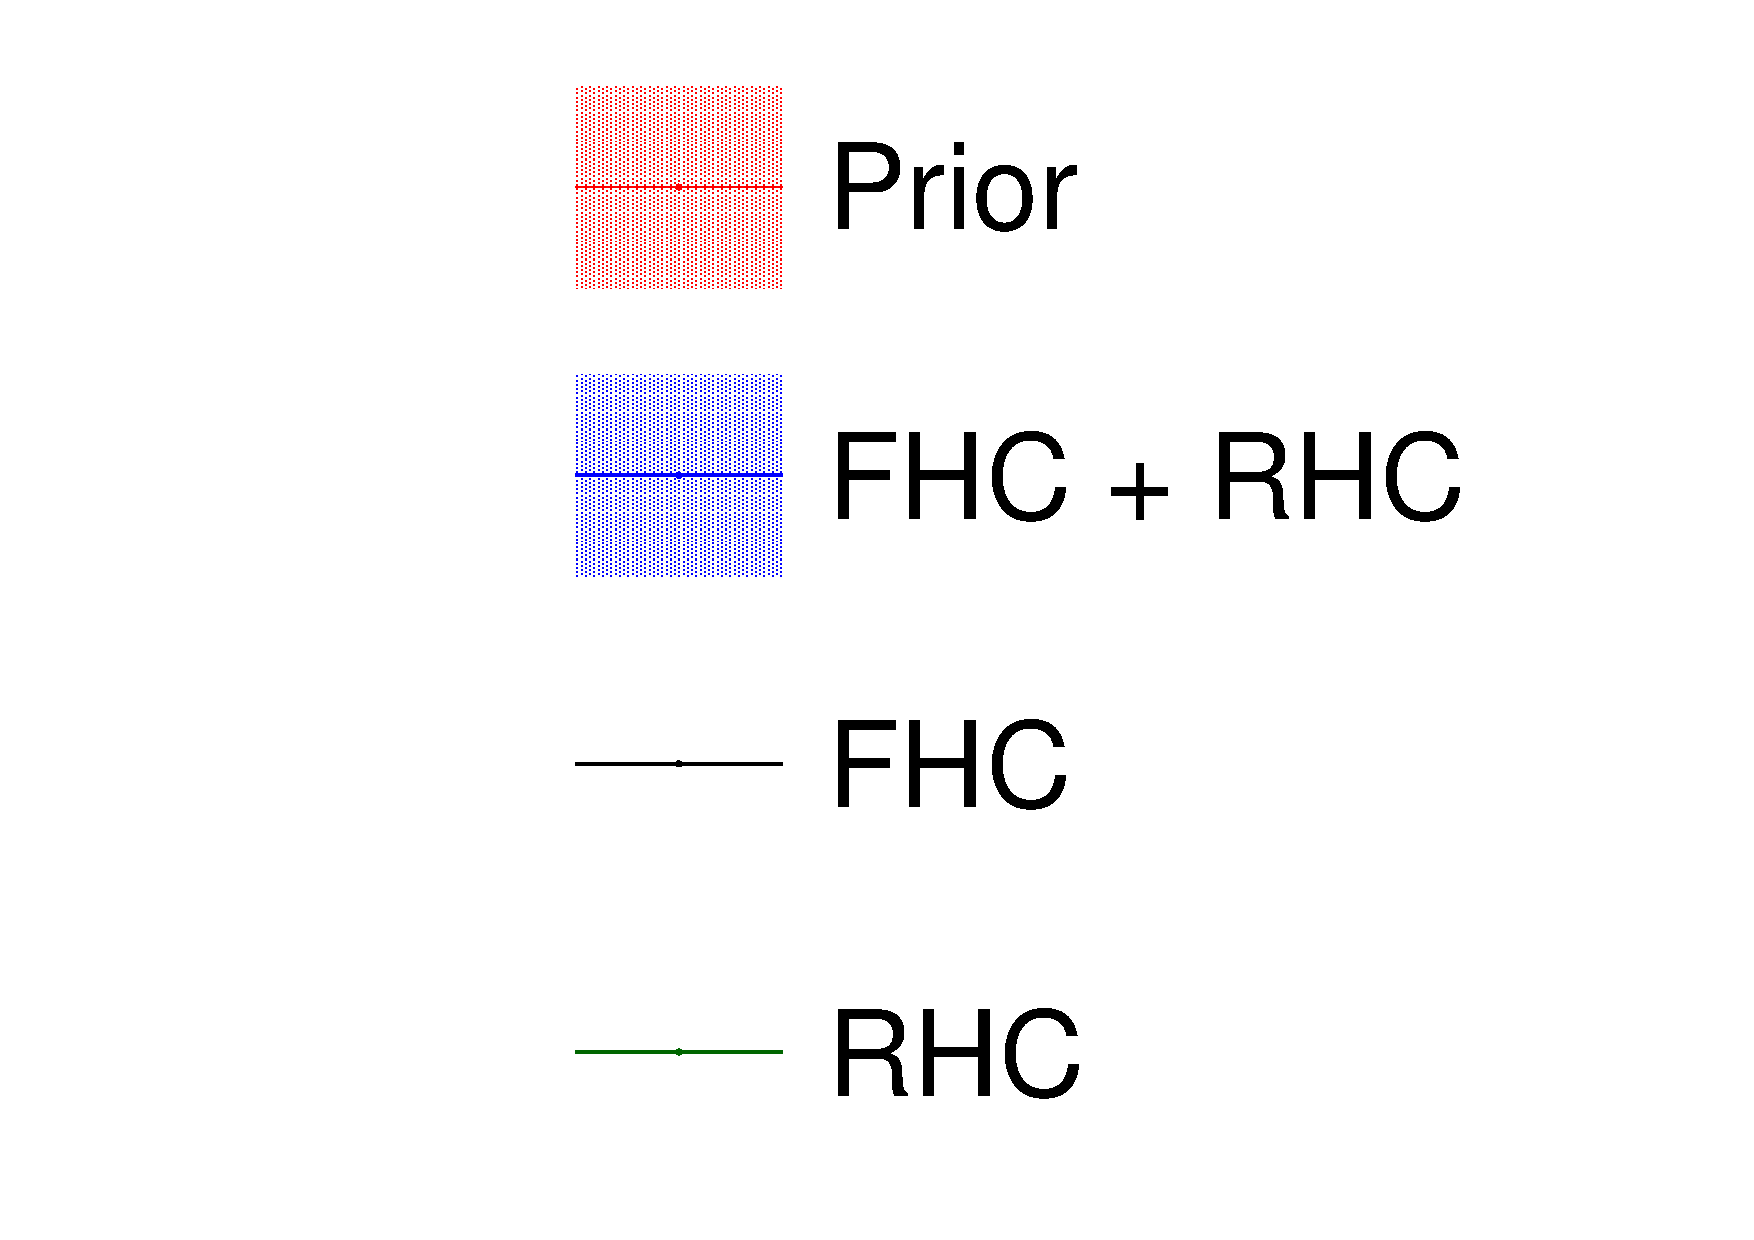
\includegraphics[width=1.0\linewidth, trim={5mm  0mm 0mm 95mm}, clip]{figs/fhcrhcfits_leg}
\end{subfigure}
\begin{subfigure}{0.45\textwidth}
  \centering
  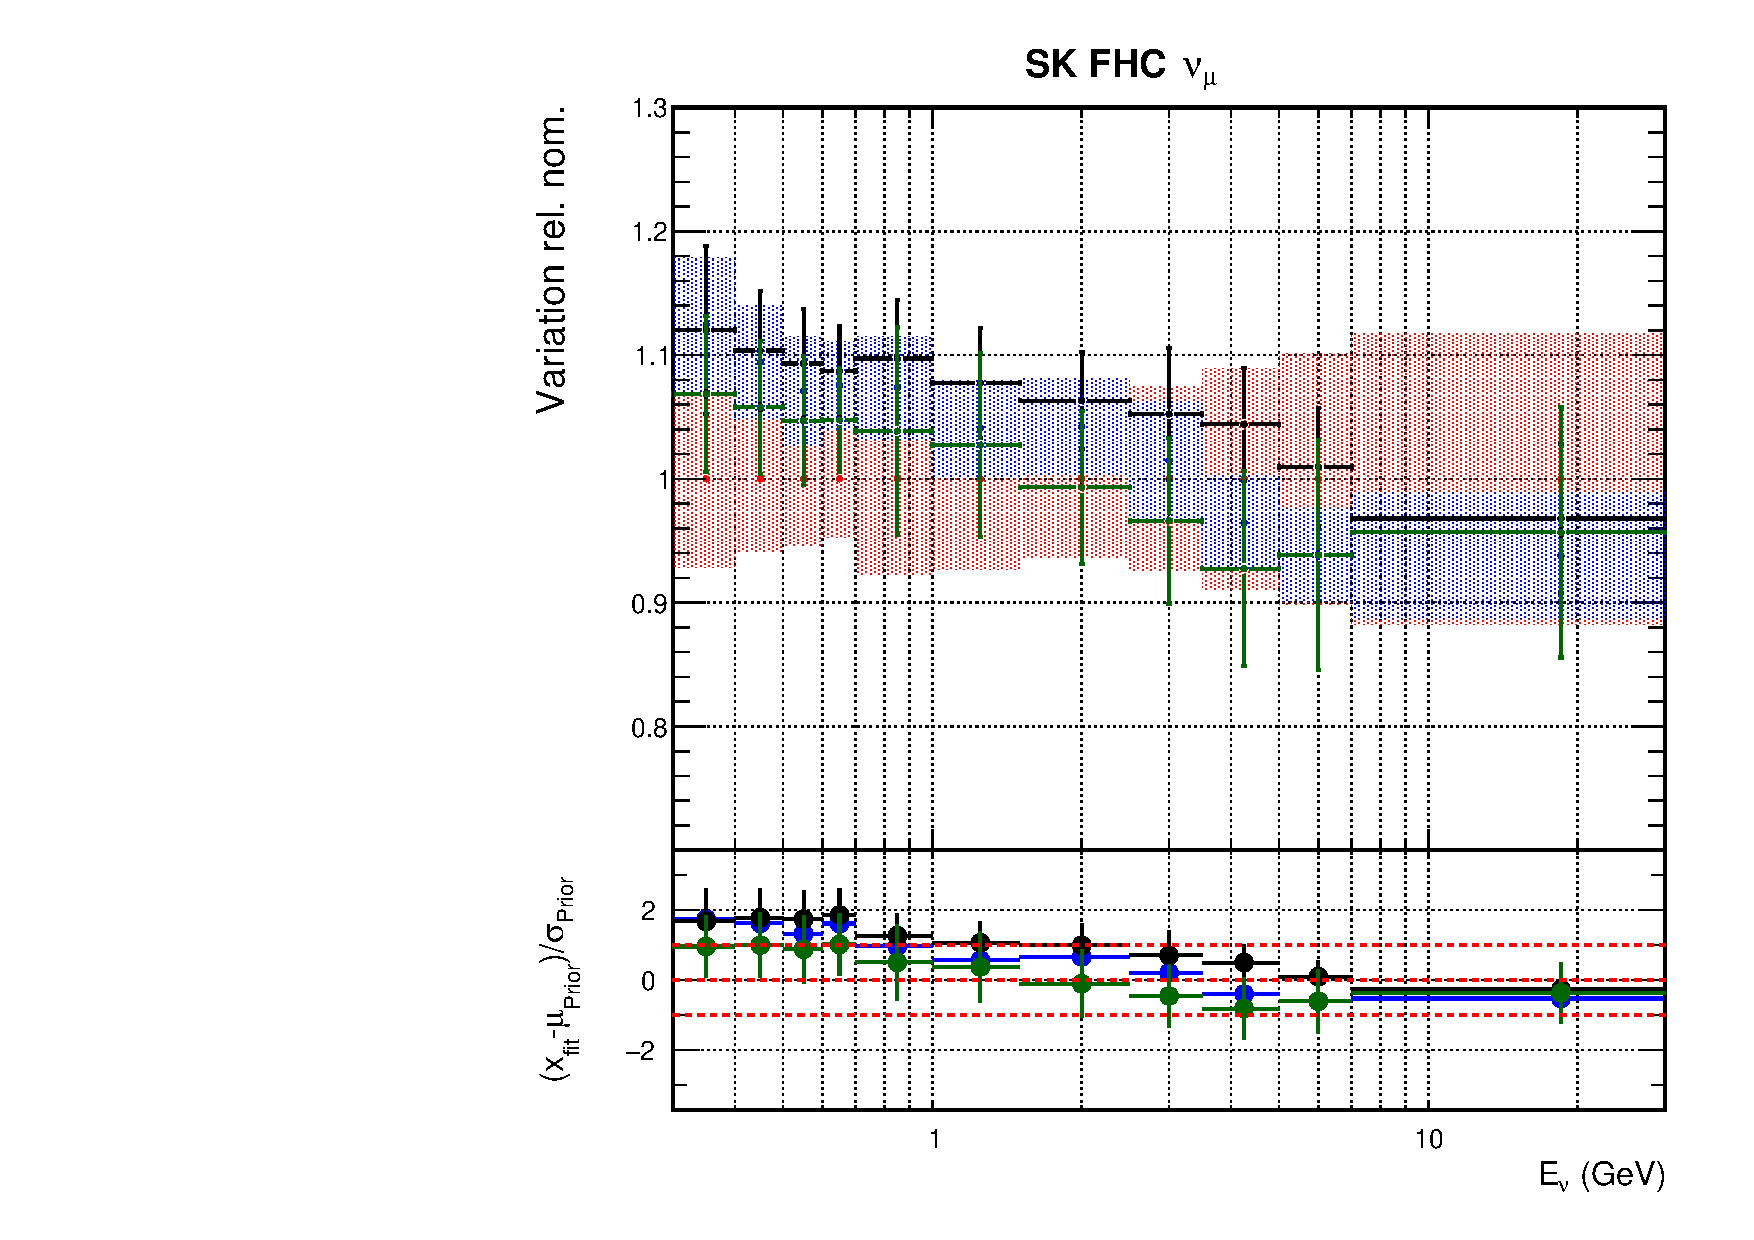
\includegraphics[width=0.75\linewidth]{figs/fhcrhcfitsflux_8}
  \caption{\SK FHC $\nu_{\mu}$}
\end{subfigure}
\begin{subfigure}{0.45\textwidth}
  \centering
  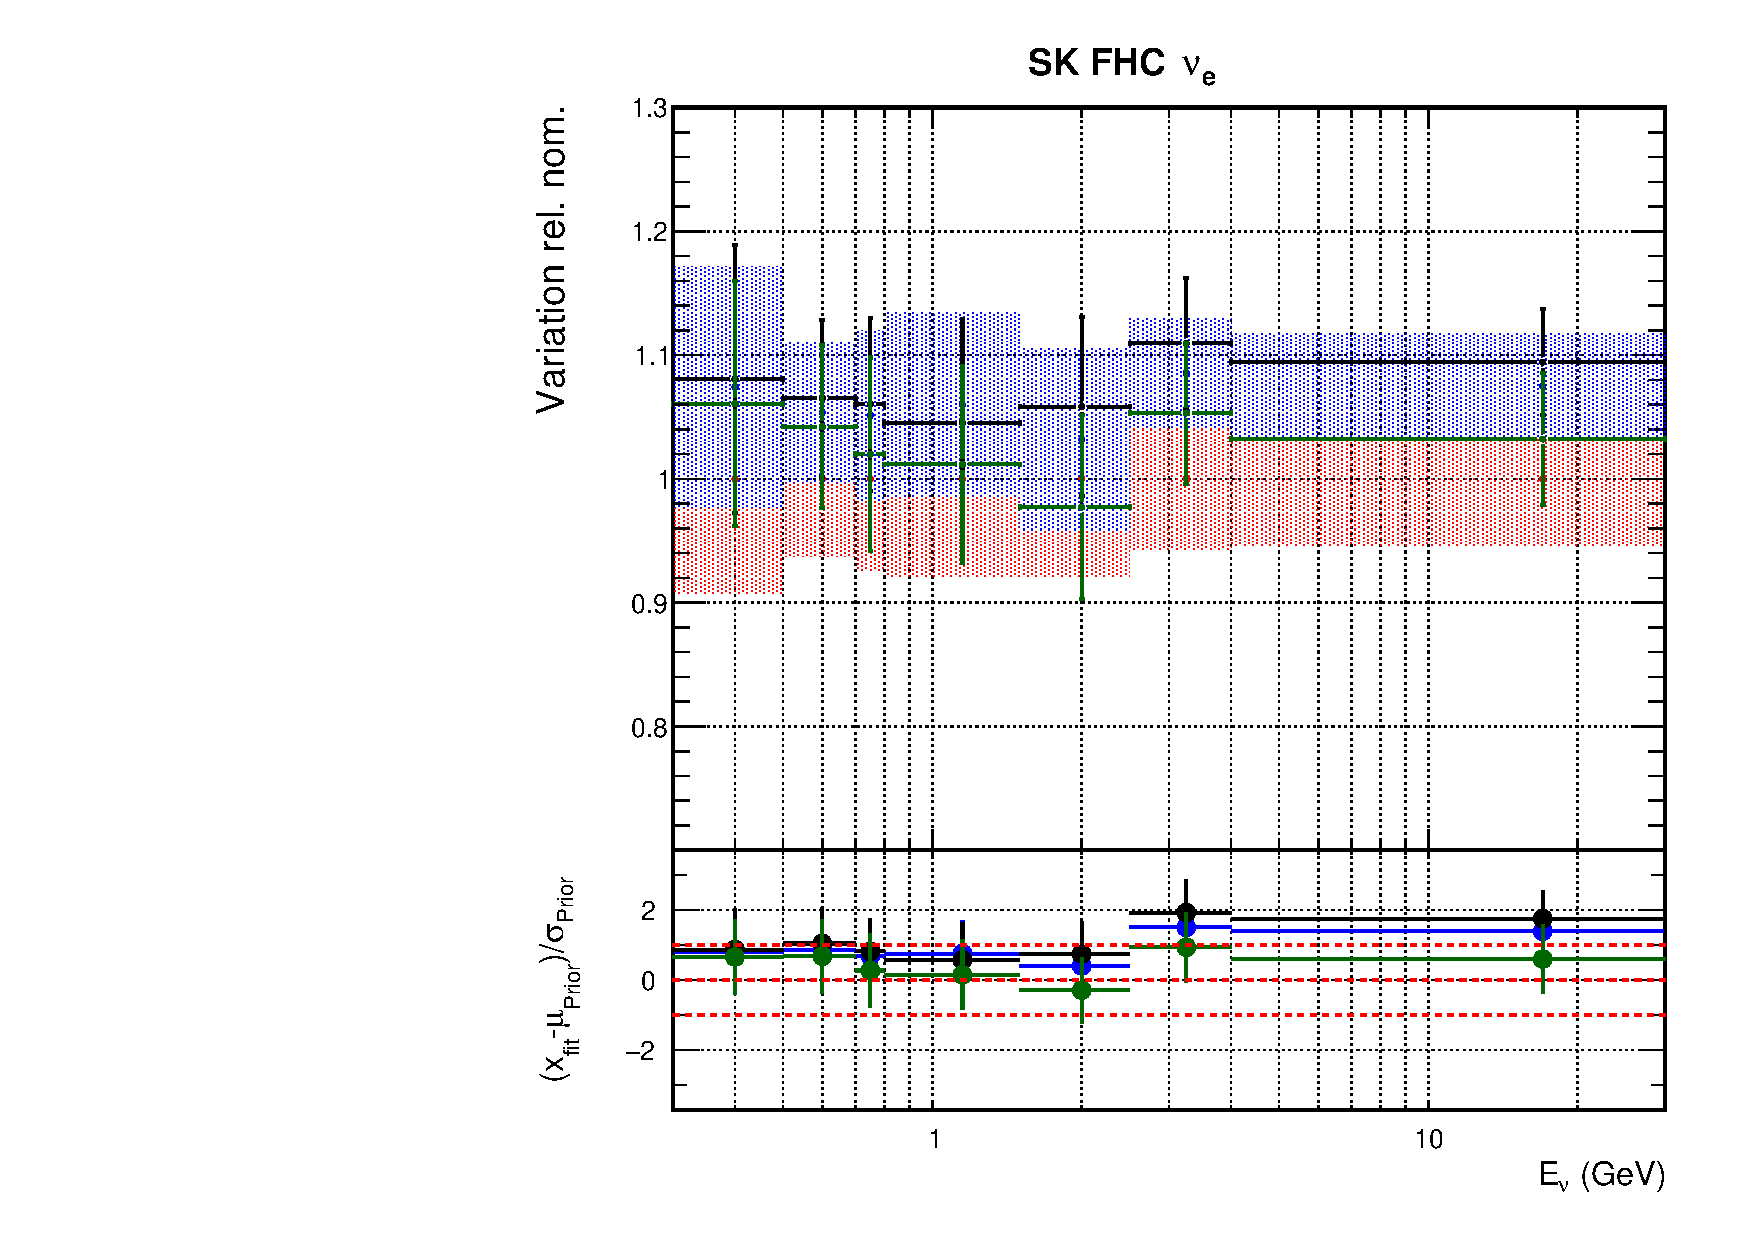
\includegraphics[width=0.75\linewidth]{figs/fhcrhcfitsflux_9}
  \caption{\SK FHC $\bar{\nu_{\mu}}$}
\end{subfigure}
\begin{subfigure}{0.45\textwidth}
  \centering
  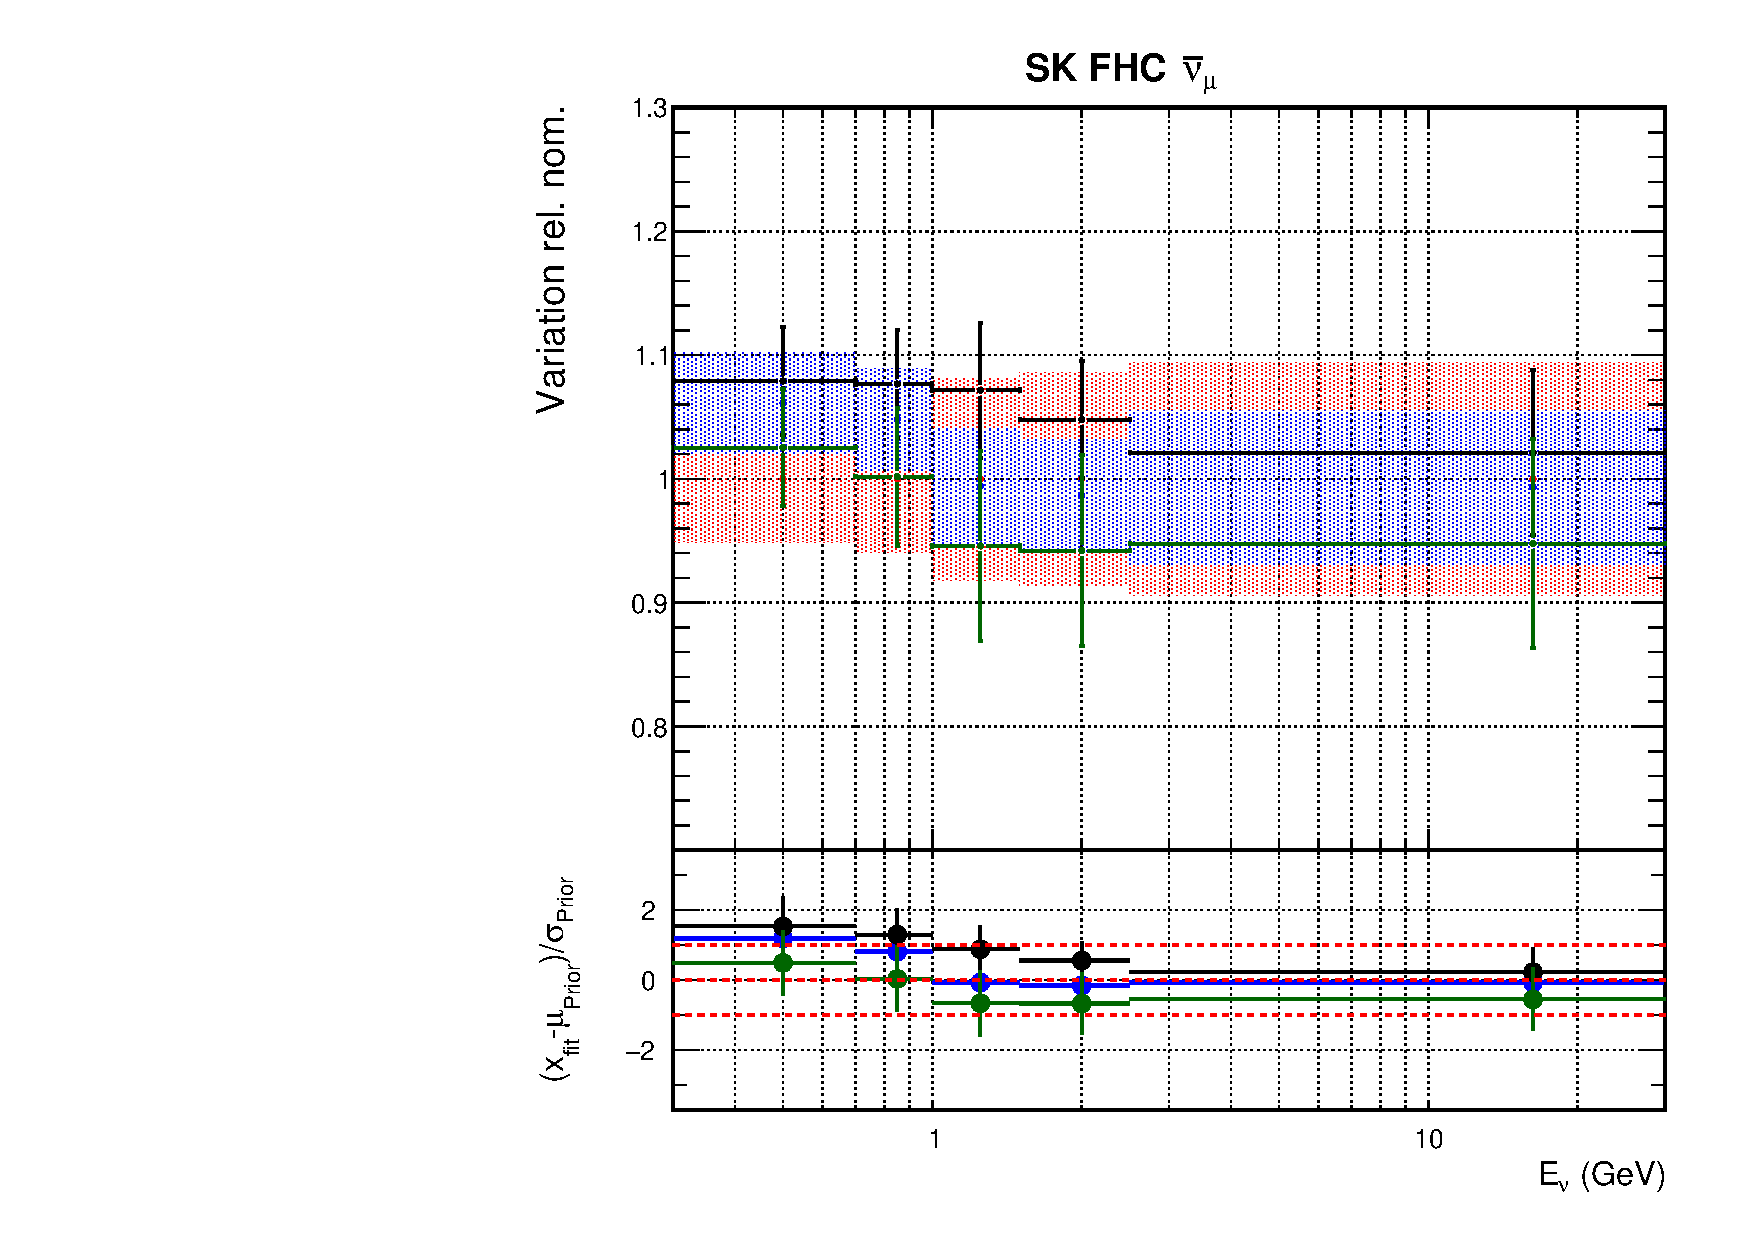
\includegraphics[width=0.75\linewidth]{figs/fhcrhcfitsflux_10}
  \caption{\SK FHC $\nu_e$}
\end{subfigure}
\begin{subfigure}{0.45\textwidth}
  \centering
  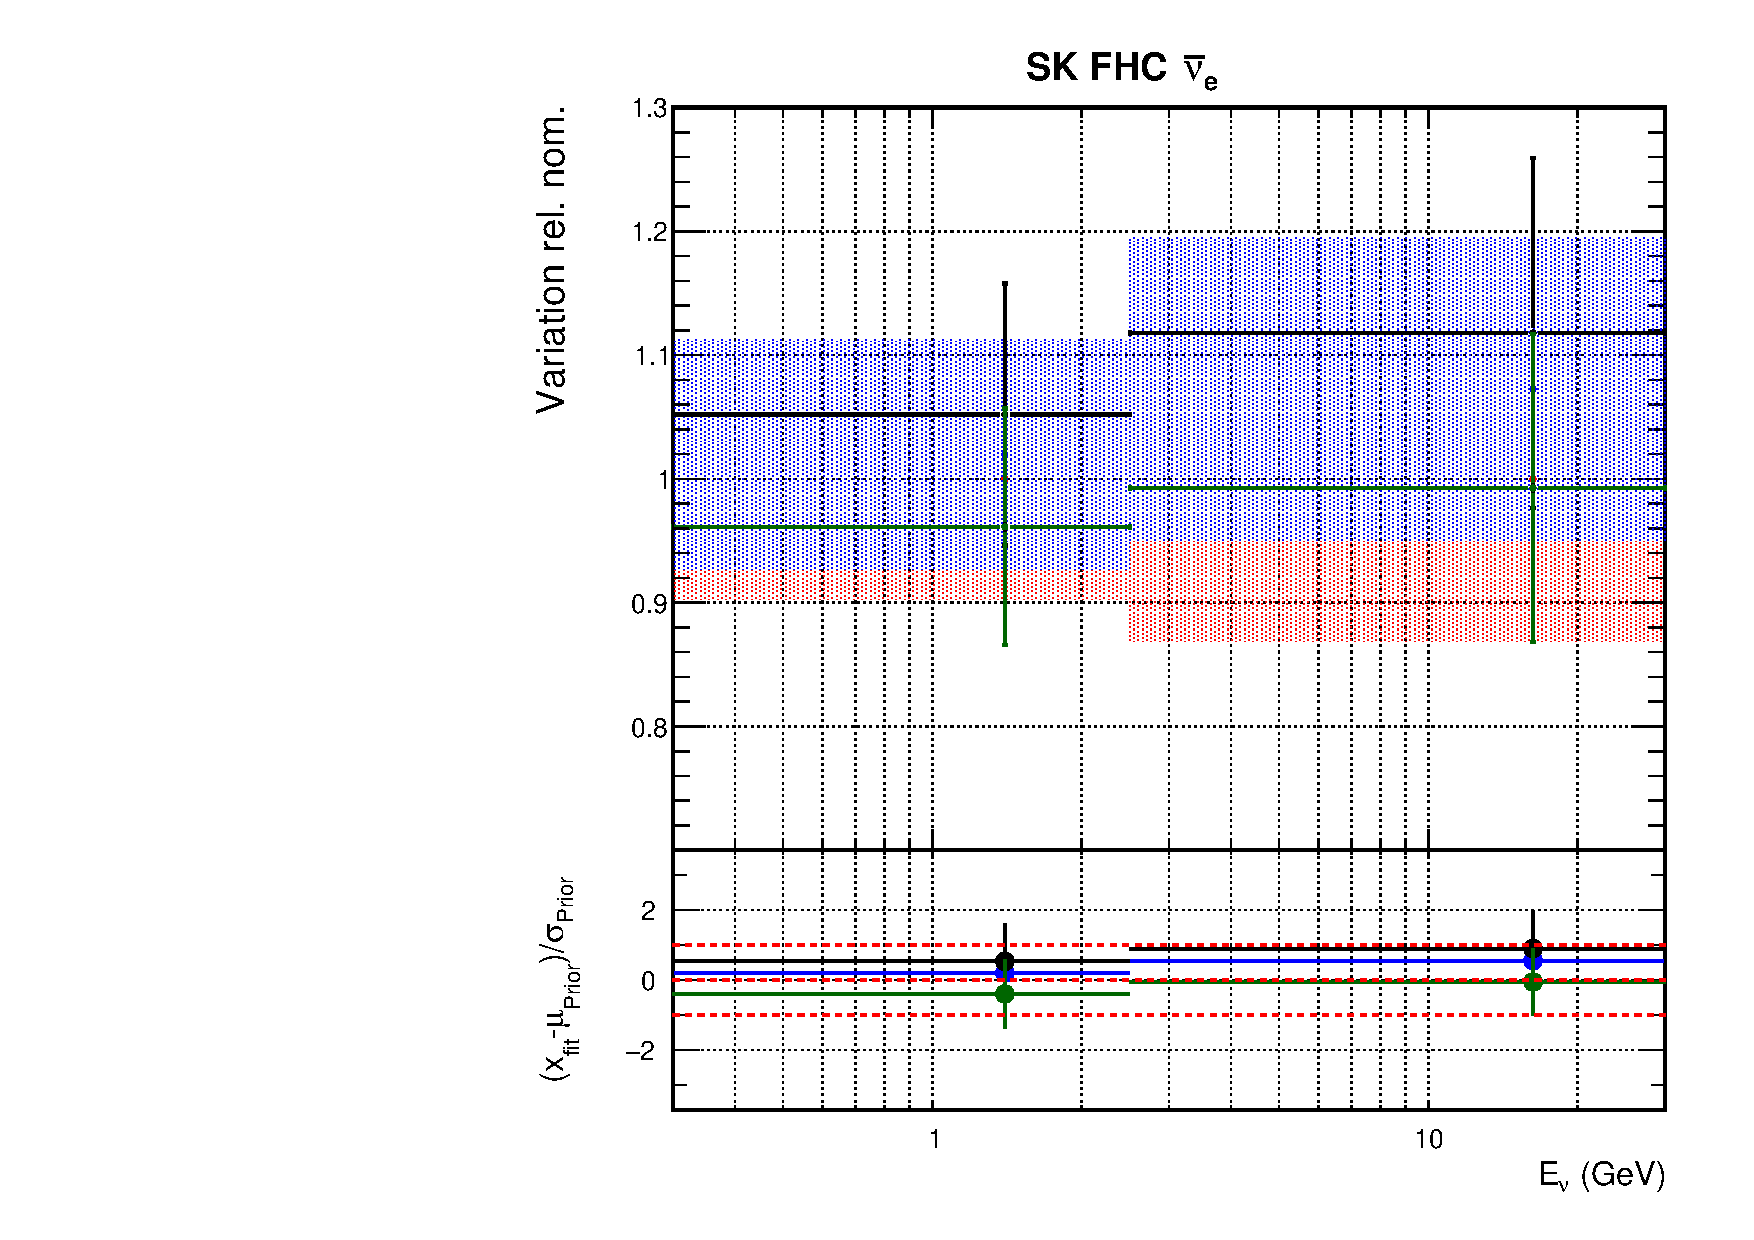
\includegraphics[width=0.75\linewidth]{figs/fhcrhcfitsflux_11}
  \caption{\SK FHC $\bar{\nu_{e}}$}
\end{subfigure}
\begin{subfigure}{0.45\textwidth}
  \centering
  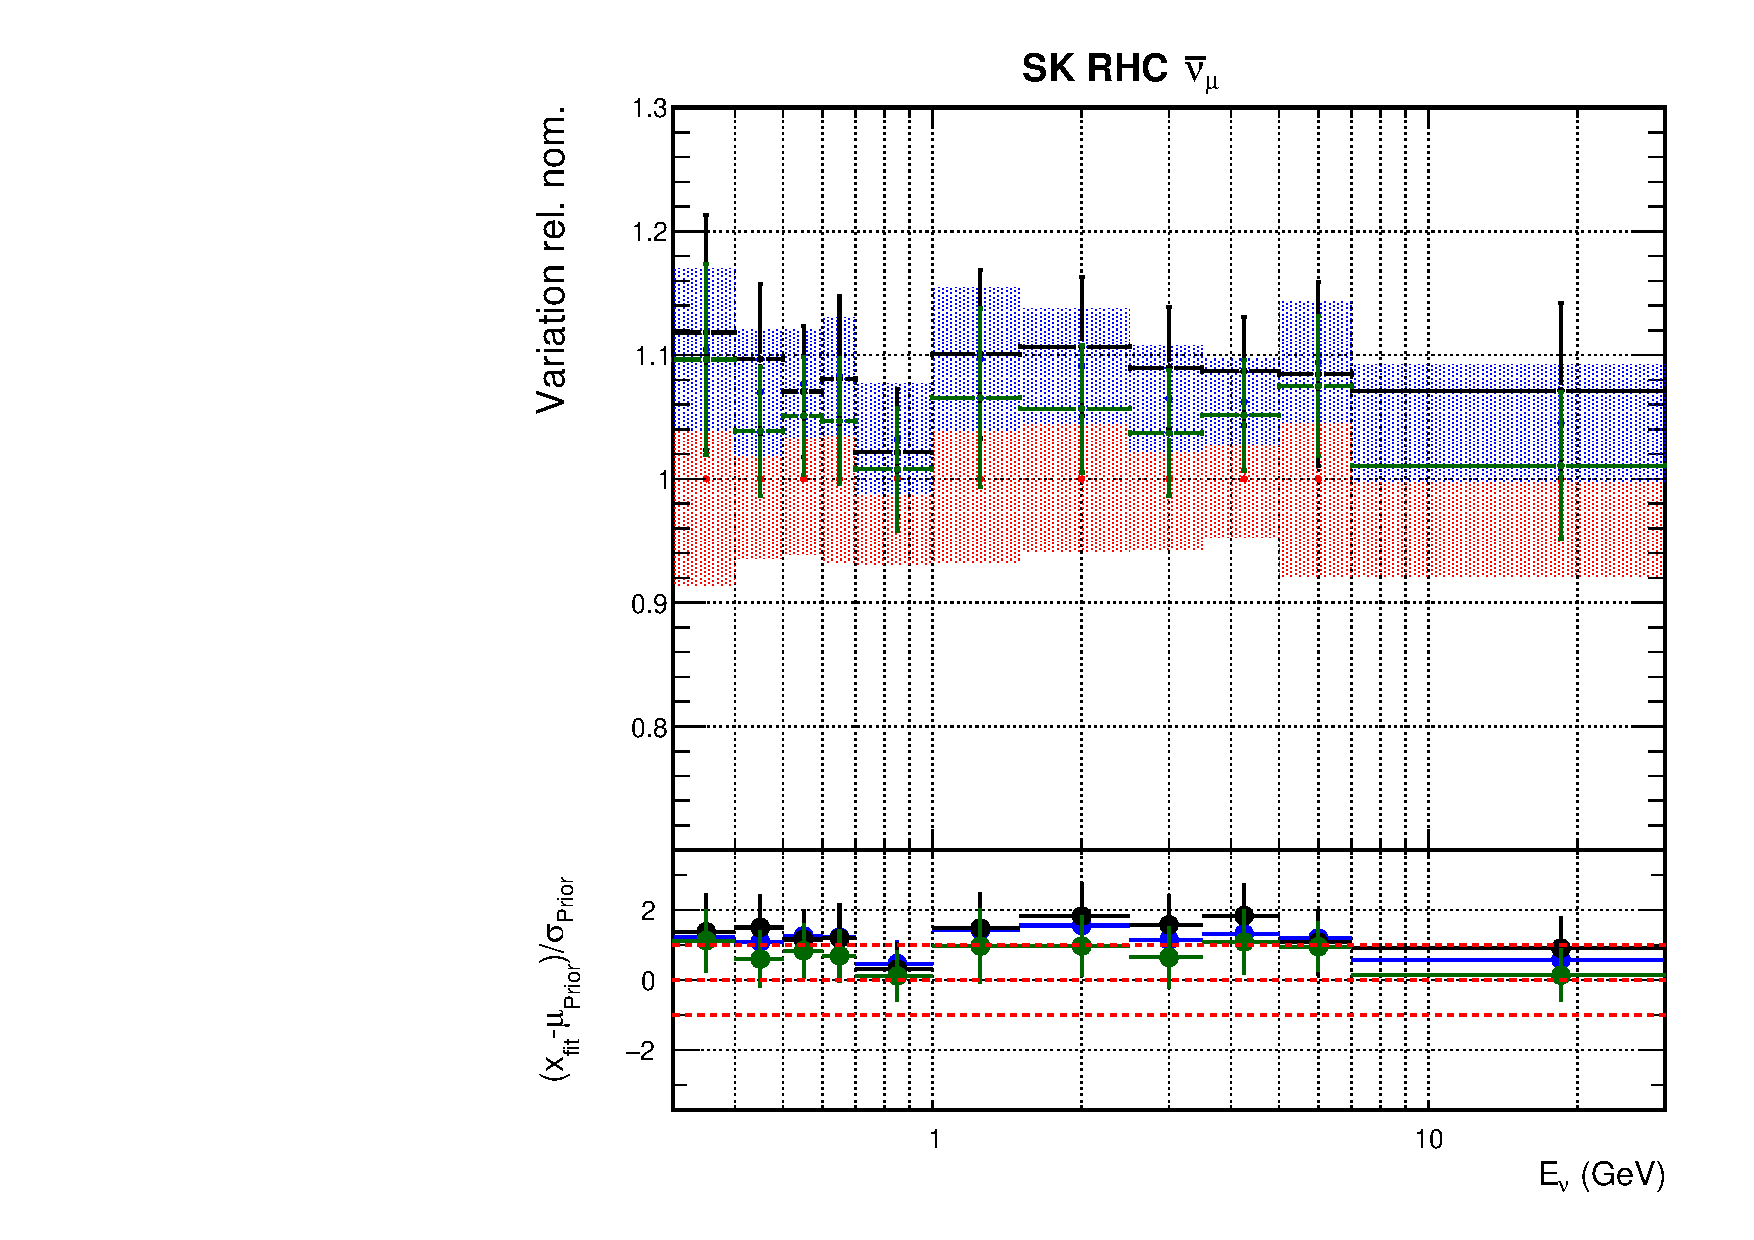
\includegraphics[width=0.75\linewidth]{figs/fhcrhcfitsflux_12}
  \caption{\SK RHC $\nu_{\mu}$}
\end{subfigure}
\begin{subfigure}{0.45\textwidth}
  \centering
  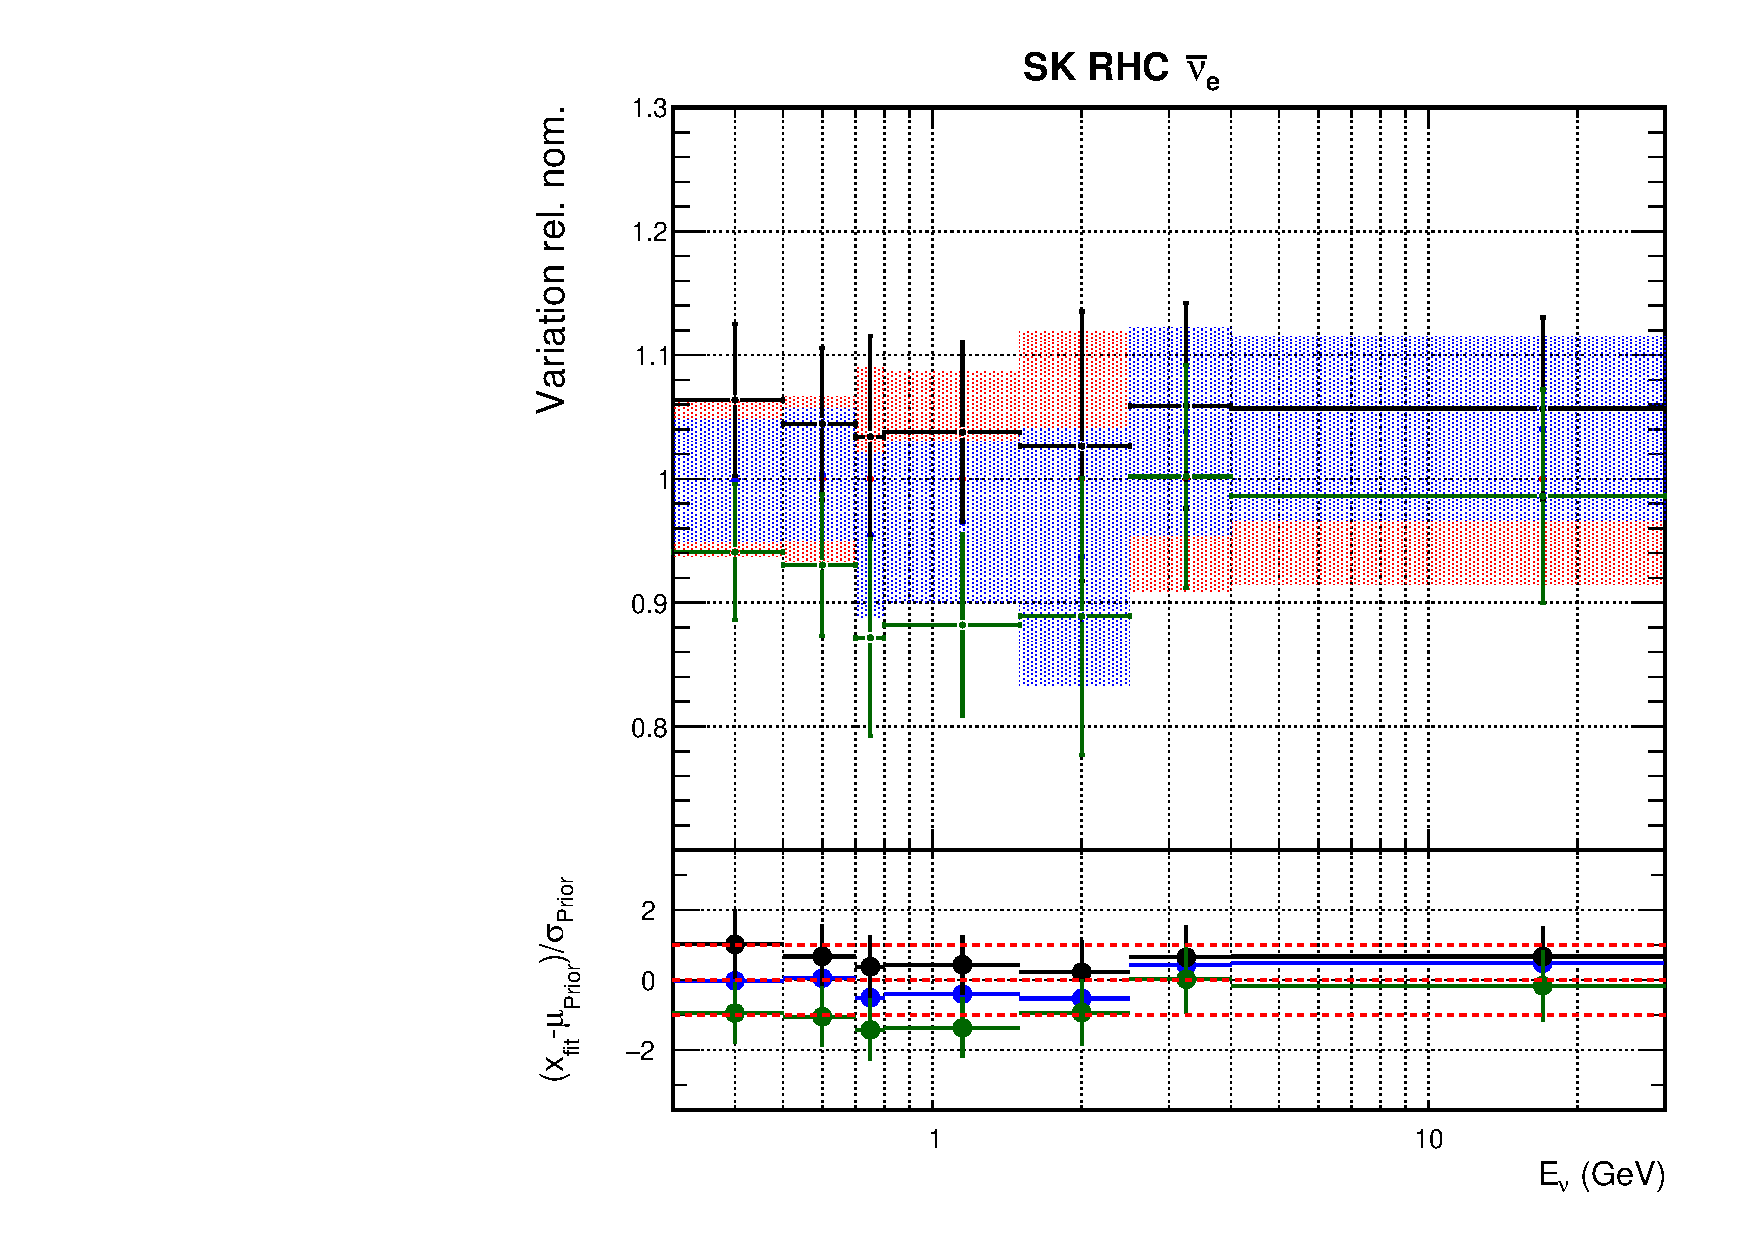
\includegraphics[width=0.75\linewidth]{figs/fhcrhcfitsflux_13}
  \caption{\SK RHC $\bar{\nu_{\mu}}$}
\end{subfigure}
\begin{subfigure}{0.45\textwidth}
  \centering
  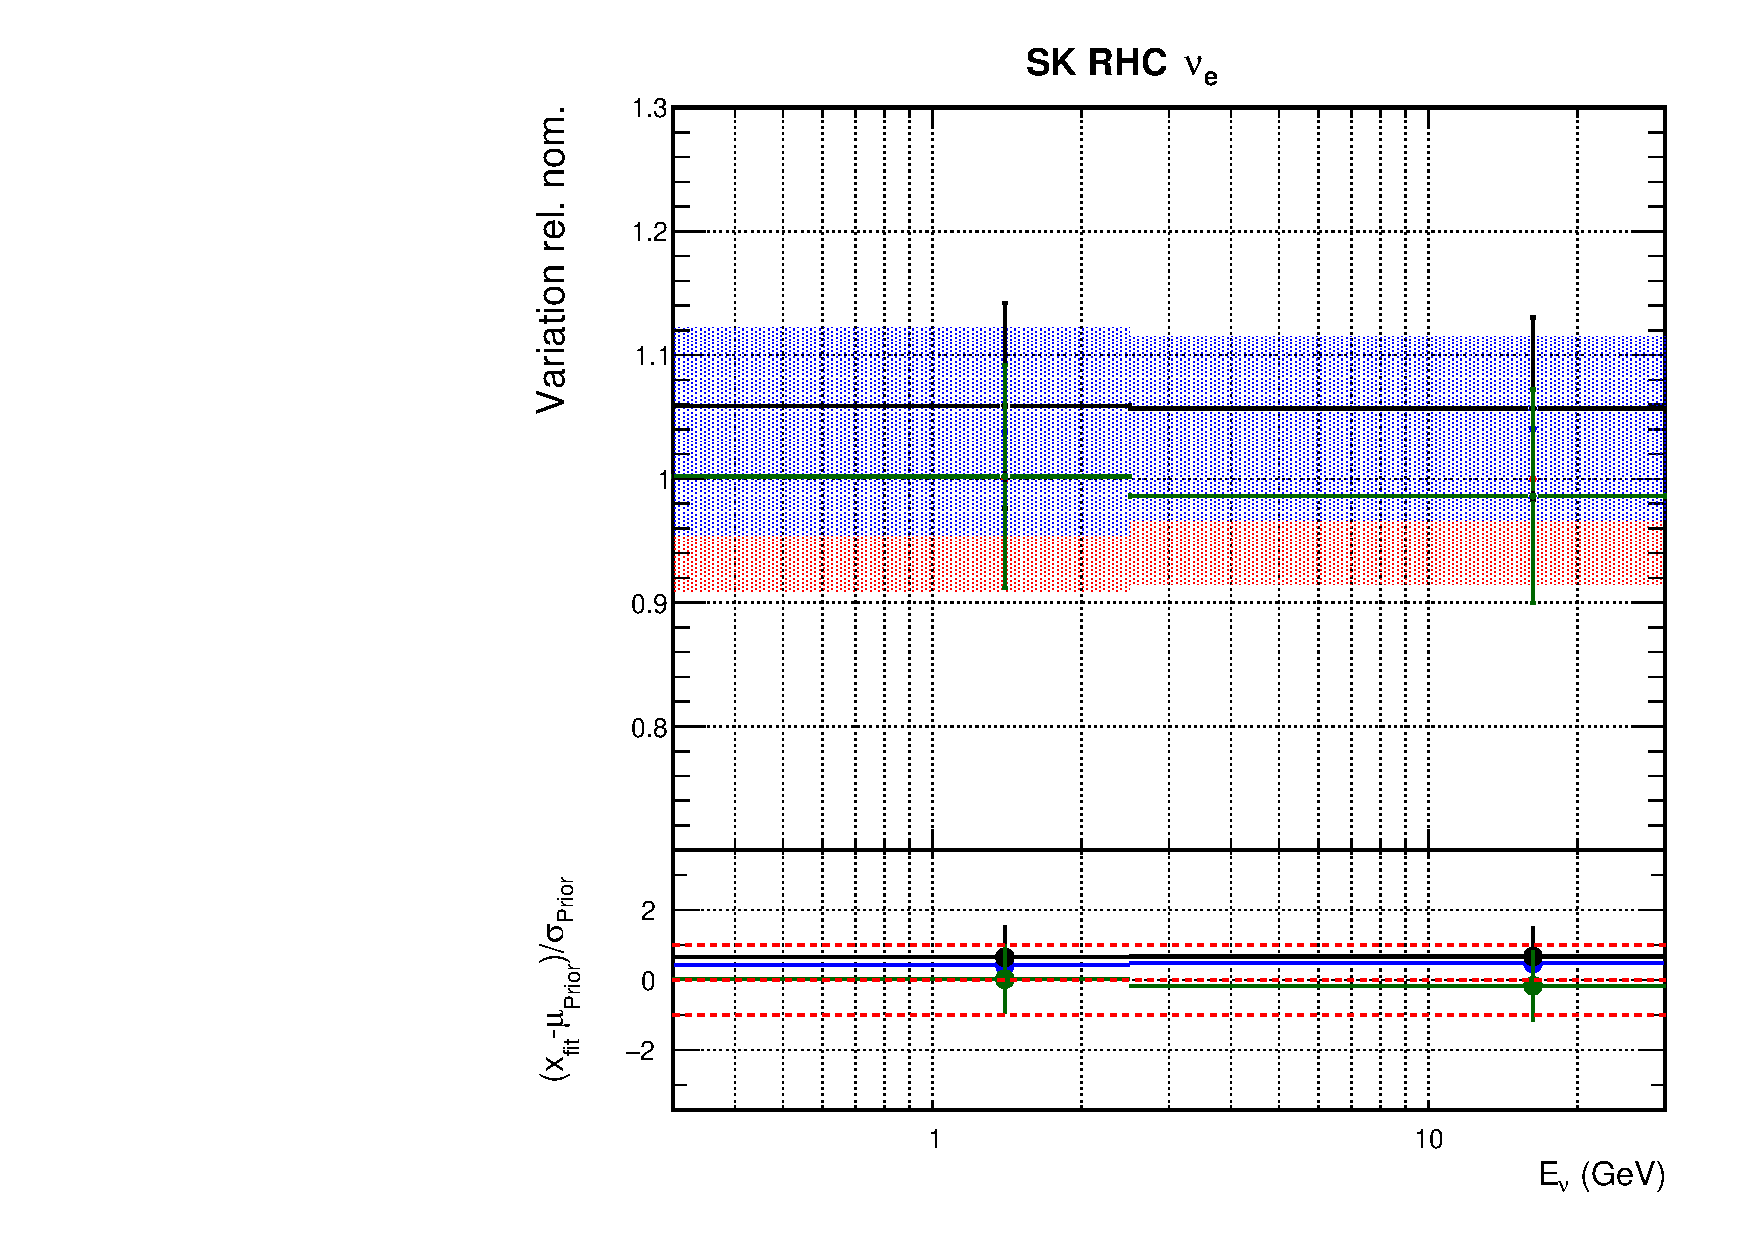
\includegraphics[width=0.75\linewidth]{figs/fhcrhcfitsflux_14}
  \caption{\SK RHC $\nu_{e}$}
\end{subfigure}
\begin{subfigure}{0.45\textwidth}
  \centering
  \includegraphics[width=0.75\linewidth]{figs/fhcrhcfitsflux_15}
  \caption{\SK RHC $\bar{\nu_e}$}
\end{subfigure}
\caption{\SK flux parameters for the FHC and RHC only fits.}
\label{fig:fhcrhcfluxSK}
\end{figure}

The results for the interaction parameters are shown in Figure \ref{fig:fhcrhcxsec}. $M_{A}^{QE}$ is not pushed as high for FHC as RHC, but both are within the postfit uncertainty of the full fit value. The 2p2h $\nu$ normalisation gets a small constraint in the RHC fit from the $\nu$ in $\bar{\nu}$ samples, but the 2p2h $\bar{\nu}$ normalisation gets no constraint in the FHC only fit. The 2p2h C to O normalisation and shape parameters for the FHC and RHC only fits are $1\sigma$ either side of the full fits. 

The $Q^2$ normalisations are closer to nominal for RHC, but the shape of the increase with increasing $Q^2$ is similar. 

\begin{figure}
\centering
\begin{subfigure}{0.3\textwidth}
  \centering
  \includegraphics[width=1.0\linewidth, trim={5mm  90mm 0mm 0mm}, clip]{figs/fhcrhcfits_leg}
\end{subfigure}
\begin{subfigure}{0.3\textwidth}
  \centering
  \includegraphics[width=1.0\linewidth, trim={5mm  0mm 0mm 95mm}, clip]{figs/fhcrhcfits_leg}
\end{subfigure}
\begin{subfigure}{0.49\textwidth}
  \centering
  \includegraphics[width=0.9\linewidth]{figs/fhcrhcfitsxsec_1}
  \caption{CC 0$\pi$}
\end{subfigure}
\begin{subfigure}{0.49\textwidth}
  \centering
  \includegraphics[width=0.9\linewidth]{figs/fhcrhcfitsxsec_2}
  \caption{$Q^2$ and $E_{\mathrm{b}}$}
\end{subfigure}
\begin{subfigure}{0.49\textwidth}
  \centering
  \includegraphics[width=0.9\linewidth]{figs/fhcrhcfitsxsec_3}
  \caption{CC 1$\pi$, $\nu_e$, CC DIS, CC multi-$\pi$ and CC Coh.}
\end{subfigure}
\begin{subfigure}{0.49\textwidth}
  \centering
  \includegraphics[width=0.9\linewidth]{figs/fhcrhcfitsxsec_4}
  \caption{NC}
\end{subfigure}
\begin{subfigure}{0.49\textwidth}
  \centering
  \includegraphics[width=0.9\linewidth]{figs/fhcrhcfitsxsec_5}
  \caption{$\pi$ FSI}
\end{subfigure}
\caption{Interaction parameters for the FHC and RHC only fits.}
\label{fig:fhcrhcxsec}
\end{figure}

The $E_{\mathrm{b}}$ distributions are shown in Figure \ref{fig:fhcrhcxsec} as they are non-Gaussian and so the single extracted values do not show the whole story. The distributions for $E_{\mathrm{b}} \nu$ C parameter are similar for the FHC and full fits, as would be expected. In the RHC fit, it is only constrained through the prior correlations to the FHC $E_{\mathrm{b}}$ parameters and the wrong-sign background samples. Similarly, $E_{\mathrm{b}} \bar{\nu}$ C is very similar for RHC only and the full fit. As there are no FHC wrong-sign samples, $E_{\mathrm{b}} \bar{\nu}$ C is only constrained through the prior uncertainty and correlations in FHC only fit, and so the postfit value is close to the prior central value. The $E_{\mathrm{b}}$ O parameters are both much more consistent across the three fits.

$M_{A}^{RES}$ is much closer to nominal for RHC, but the full fit favours the FHC value. The BY parameters are both also closer to nominal for RHC, with the full fit values lying between the FHC and RHC only values. The NC parameters are all consistent for the fits, and of the FSI parameters, high energy quasi-elastic is the only systematic for which the postfit values are outside $1\sigma$ of each other, with the full fit favouring the FHC value.

Overall these fits show some tension, with the postfit values being generally closer to nominal for RHC only. However, this is likely because there are lower statistics for RHC, so the contribution to the likelihood from the prior uncertainty becomes more significant.

\begin{figure}
\centering
\begin{subfigure}{.48\textwidth}
  \centering
  \includegraphics[width=0.73\linewidth]{figs/FHCRHC_EB_dial_C_nu}
  \caption{$E_{\mathrm{b}}\nu$ C}
\end{subfigure}
\begin{subfigure}{.48\textwidth}
  \centering
  \includegraphics[width=0.73\linewidth]{figs/FHCRHC_EB_dial_C_nubar}
  \caption{$E_{\mathrm{b}}\bar{\nu}$ C}
\end{subfigure} \\
\begin{subfigure}{.48\textwidth}
  \centering
  \includegraphics[width=0.73\linewidth]{figs/FHCRHC_EB_dial_O_nu}
  \caption{$E_{\mathrm{b}}\nu$ O}
\end{subfigure}
\begin{subfigure}{.48\textwidth}
  \centering
  \includegraphics[width=0.73\linewidth]{figs/FHCRHC_EB_dial_O_nubar}
  \caption{$E_{\mathrm{b}}\bar{\nu}$ O}
\end{subfigure}
\caption{Posterior distributions from the binding energy parameters for the FHC and RHC only fits.}
\label{fig:FHCRHCEbdata}
\end{figure}

\section{New and Old Data Only Fits}

The previous oscillation analysis\cite{PhysRevLett.121.171802} used data from runs 2--6. The addition of runs 7, 8 and 9 for this analysis approximately doubles both the FHC and RHC data. To investigate the compatibility of the new and old data, fits were run using data from just runs 2--6, and just runs 7--9. This will show if unexpected results are coming from the changes in the model or the extra data. There is approximately the same amount of data in each set, and so the constraint is expected to be similar.

The results for the flux parameters are shown in Figures \ref{fig:newolddatafluxND} and \ref{fig:newolddatafluxSK}. They are mostly consistent between the three fits, with the postfit parameters lying within the uncertainty of each other. For runs 7--9, the fluxes tend to be slightly closer to nominal, but the overall shape of the pulls in energy are similar.

\begin{figure}
\centering
\begin{subfigure}{0.3\textwidth}
  \centering
  \includegraphics[width=1.0\linewidth, trim={5mm  90mm 0mm 0mm}, clip]{figs/newolddatafits_leg}
\end{subfigure}
\begin{subfigure}{0.3\textwidth}
  \centering
  \includegraphics[width=1.0\linewidth, trim={5mm  0mm 0mm 95mm}, clip]{figs/newolddatafits_leg}
\end{subfigure}
\begin{subfigure}{0.45\textwidth}
  \centering
  \includegraphics[width=0.75\linewidth]{figs/newolddatafitsflux_0}
  \caption{ND FHC $\nu_{\mu}$}
\end{subfigure}
\begin{subfigure}{0.45\textwidth}
  \centering
  \includegraphics[width=0.75\linewidth]{figs/newolddatafitsflux_1}
  \caption{ND FHC $\bar{\nu_{\mu}}$}
\end{subfigure}
\begin{subfigure}{0.45\textwidth}
  \centering
  \includegraphics[width=0.75\linewidth]{figs/newolddatafitsflux_2}
  \caption{ND FHC $\nu_e$}
\end{subfigure}
\begin{subfigure}{0.45\textwidth}
  \centering
  \includegraphics[width=0.75\linewidth]{figs/newolddatafitsflux_3}
  \caption{ND FHC $\bar{\nu_{e}}$}
\end{subfigure}
\begin{subfigure}{0.45\textwidth}
  \centering
  \includegraphics[width=0.75\linewidth]{figs/newolddatafitsflux_4}
  \caption{ND RHC $\nu_{\mu}$}
\end{subfigure}
\begin{subfigure}{0.45\textwidth}
  \centering
  \includegraphics[width=0.75\linewidth]{figs/newolddatafitsflux_5}
  \caption{ND RHC $\bar{\nu_{\mu}}$}
\end{subfigure}
\begin{subfigure}{0.45\textwidth}
  \centering
  \includegraphics[width=0.75\linewidth]{figs/newolddatafitsflux_6}
  \caption{ND RHC $\nu_{e}$}
\end{subfigure}
\begin{subfigure}{0.45\textwidth}
  \centering
  \includegraphics[width=0.75\linewidth]{figs/newolddatafitsflux_7}
  \caption{ND RHC $\bar{\nu_e}$}
\end{subfigure}
\caption{ND280 flux parameters for the new and old data only fits.}
\label{fig:newolddatafluxND}
\end{figure}

\begin{figure}
\centering
\begin{subfigure}{0.3\textwidth}
  \centering
  \includegraphics[width=1.0\linewidth, trim={5mm  90mm 0mm 0mm}, clip]{figs/newolddatafits_leg}
\end{subfigure}
\begin{subfigure}{0.3\textwidth}
  \centering
  \includegraphics[width=1.0\linewidth, trim={5mm  0mm 0mm 95mm}, clip]{figs/newolddatafits_leg}
\end{subfigure}
\begin{subfigure}{0.45\textwidth}
  \centering
  \includegraphics[width=0.75\linewidth]{figs/newolddatafitsflux_8}
  \caption{\SK FHC $\nu_{\mu}$}
\end{subfigure}
\begin{subfigure}{0.45\textwidth}
  \centering
  \includegraphics[width=0.75\linewidth]{figs/newolddatafitsflux_9}
  \caption{\SK FHC $\bar{\nu_{\mu}}$}
\end{subfigure}
\begin{subfigure}{0.45\textwidth}
  \centering
  \includegraphics[width=0.75\linewidth]{figs/newolddatafitsflux_10}
  \caption{\SK FHC $\nu_{e}$}
\end{subfigure}
\begin{subfigure}{0.45\textwidth}
  \centering
  \includegraphics[width=0.75\linewidth]{figs/newolddatafitsflux_11}
  \caption{\SK FHC $\bar{\nu_{e}}$}
\end{subfigure}
\begin{subfigure}{0.45\textwidth}
  \centering
  \includegraphics[width=0.75\linewidth]{figs/newolddatafitsflux_12}
  \caption{\SK RHC $\nu_{\mu}$}
\end{subfigure}
\begin{subfigure}{0.45\textwidth}
  \centering
  \includegraphics[width=0.75\linewidth]{figs/newolddatafitsflux_13}
  \caption{\SK RHC $\bar{\nu_{\mu}}$}
\end{subfigure}
\begin{subfigure}{0.45\textwidth}
  \centering
  \includegraphics[width=0.75\linewidth]{figs/newolddatafitsflux_14}
  \caption{\SK RHC $\nu_{e}$}
\end{subfigure}
\begin{subfigure}{0.45\textwidth}
  \centering
  \includegraphics[width=0.75\linewidth]{figs/newolddatafitsflux_15}
  \caption{\SK RHC $\bar{\nu_e}$}
\end{subfigure}
\caption{\SK flux parameters for the new and old data only fits.}
\label{fig:newolddatafluxSK}
\end{figure}

The interaction parameters, shown in Figure \ref{fig:newolddataxsec}, show more differences between the fits. $M_{A}^{QE}$ is very consistent, but the 2p2h normalisations are both closer to nominal for runs 2--6, as is 2p2h shape C. Interestingly, the full fit value for 2p2h shape C to O is beyond both the subset fits. The $Q^2$ normalisations are all very similar for the three fits.

\begin{figure}
\centering
\begin{subfigure}{0.3\textwidth}
  \centering
  \includegraphics[width=1.0\linewidth, trim={5mm  90mm 0mm 0mm}, clip]{figs/newolddatafits_leg}
\end{subfigure}
\begin{subfigure}{0.3\textwidth}
  \centering
  \includegraphics[width=1.0\linewidth, trim={5mm  0mm 0mm 95mm}, clip]{figs/newolddatafits_leg}
\end{subfigure}
\begin{subfigure}{0.49\textwidth}
  \centering
  \includegraphics[width=0.9\linewidth]{figs/newolddatafitsxsec_1}
  \caption{CC 0$\pi$}
\end{subfigure}
\begin{subfigure}{0.49\textwidth}
  \centering
  \includegraphics[width=0.9\linewidth]{figs/newolddatafitsxsec_2}
  \caption{$Q^2$ and $E_{\mathrm{b}}$}
\end{subfigure}
\begin{subfigure}{0.49\textwidth}
  \centering
  \includegraphics[width=0.9\linewidth]{figs/newolddatafitsxsec_3}
  \caption{CC 1$\pi$, $\nu_e$, CC DIS, CC multi-$\pi$ and CC Coh.}
\end{subfigure}
\begin{subfigure}{0.49\textwidth}
  \centering
  \includegraphics[width=0.9\linewidth]{figs/newolddatafitsxsec_4}
  \caption{NC}
\end{subfigure}
\begin{subfigure}{0.49\textwidth}
  \centering
  \includegraphics[width=0.9\linewidth]{figs/newolddatafitsxsec_5}
  \caption{$\pi$ FSI}
\end{subfigure}
\caption{Interaction parameters for the new and old data only fits.}
\label{fig:newolddataxsec}
\end{figure}

The $E_{\mathrm{b}}$ distributions are shown in Figure \ref{fig:RunsEbdata}, as they are non-Gaussian and so the single extracted values alone are not sufficient. The $E_{\mathrm{b}} \nu$ C and $E_{\mathrm{b}} \nu$ O parameters both have large peaks at higher values for runs 2--6. The full fit prefers the runs 7--9 value for C, and the runs 2--6 value for O. The full fit distributions for the $E_{\mathrm{b}} \bar{\nu}$ C and $E_{\mathrm{b}} \bar{\nu}$ O parameters are both similar to those for runs 7--9. The distributions for runs 2--6 have more peaks, but center around similar values.

As runs 2--6 have a larger proportion of FHC data, it would be expected that more of the full fit constraint on $\nu$ parameters would be coming from runs 2--6, and more of the full fit constraint on $\bar{\nu}$ parameters would be coming from runs 7--9. However, there does not seem to be a general trend of the full fit parameters for $\nu$ or $\bar{\nu}$ being closer to the runs 2--6 or 7--9 values. This is probably because the proportions of FHC/RHC data in each set are vastly different, and so other factors dominate.

For runs 7--9, CC DIS BY is higher and CC BY multi-$\pi$, CC AGKY mult., and CC misc. are lower than for runs 2--6, with the full fit values lying between the two. The rest of the CC $1\pi$ and CC Other targetting parameters are fairly consistent. The inelastic and charge exchange FSI parameters are both closer to nominal for runs 7--9.

Overall, there is some tension between these fits, but nearly all parameters are within $1\sigma$ of the each other. In most cases, the full fit value lies between the runs 2--6 and 7--9 values.

\begin{figure}
\centering
\begin{subfigure}{.48\textwidth}
  \centering
  \includegraphics[width=0.73\linewidth]{figs/Runs_EB_dial_C_nu}
  \caption{$E_{\mathrm{b}}\nu$ C}
\end{subfigure}
\begin{subfigure}{.48\textwidth}
  \centering
  \includegraphics[width=0.73\linewidth]{figs/Runs_EB_dial_C_nubar}
  \caption{$E_{\mathrm{b}}\bar{\nu}$ C}
\end{subfigure} \\
\begin{subfigure}{.48\textwidth}
  \centering
  \includegraphics[width=0.73\linewidth]{figs/Runs_EB_dial_O_nu}
  \caption{$E_{\mathrm{b}}\nu$ O}
\end{subfigure}
\begin{subfigure}{.48\textwidth}
  \centering
  \includegraphics[width=0.73\linewidth]{figs/Runs_EB_dial_O_nubar}
  \caption{$E_{\mathrm{b}}\bar{\nu}$ O}
\end{subfigure}
\caption{Posterior distributions from the binding energy parameters for the new and old data only fits.}
\label{fig:RunsEbdata}
\end{figure}

\section{Flat MAQE Prior and Less $Q^2$ Freedom}

Two interaction models were proposed for this analysis. As $M_{A}^{QE}$ affects events with high $Q^{2}$, one model had only five $Q^2$ normalisations (up to 0.25 GeV), but with a flat prior on $M_{A}^{QE}$. The other model invoked a tight prior uncertainty of 0.06 GeV$^2$ on $M_{A}^{QE}$, but had extra high $Q^2$ freedom from the three additional high $Q^2$ normalisations. Fits were ran with both these models.

The comparison of the results for the flux parameters are shown in Figures \ref{fig:comp5q2vs8q2fluxND} and \ref{fig:comp5q2vs8q2fluxSK}. The shape of the pulls in energy are similar for the two fits, but the fluxes are generally slightly lower for the fit with eight $Q^2$ normalisations.

Similar results are seen for the ND280 and \SK flux parameters, as would be expected.

\begin{figure}
\centering
\begin{subfigure}{0.3\textwidth}
  \centering
  \includegraphics[width=1.0\linewidth, trim={5mm  130mm 0mm 10mm}, clip]{figs/comp5q2vs8q2_leg}
\end{subfigure}
\begin{subfigure}{0.3\textwidth}
  \centering
  \includegraphics[width=1.0\linewidth, trim={5mm  0mm 0mm 70mm}, clip]{figs/comp5q2vs8q2_leg}
\end{subfigure}
\begin{subfigure}{0.45\textwidth}
  \centering
  \includegraphics[width=0.75\linewidth]{figs/comp5q2vs8q2flux0}
  \caption{ND FHC $\nu_{\mu}$}
\end{subfigure}
\begin{subfigure}{0.45\textwidth}
  \centering
  \includegraphics[width=0.75\linewidth]{figs/comp5q2vs8q2flux1}
  \caption{ND FHC $\bar{\nu_{\mu}}$}
\end{subfigure}
\begin{subfigure}{0.45\textwidth}
  \centering
  \includegraphics[width=0.75\linewidth]{figs/comp5q2vs8q2flux2}
  \caption{ND FHC $\nu_{e}$}
\end{subfigure}
\begin{subfigure}{0.45\textwidth}
  \centering
  \includegraphics[width=0.75\linewidth]{figs/comp5q2vs8q2flux3}
  \caption{ND FHC $\bar{\nu_{e}}$}
\end{subfigure}
\begin{subfigure}{0.45\textwidth}
  \centering
  \includegraphics[width=0.75\linewidth]{figs/comp5q2vs8q2flux4}
  \caption{ND RHC $\nu_{\mu}$}
\end{subfigure}
\begin{subfigure}{0.45\textwidth}
  \centering
  \includegraphics[width=0.75\linewidth]{figs/comp5q2vs8q2flux5}
  \caption{ND RHC $\bar{\nu_{\mu}}$}
\end{subfigure}
\begin{subfigure}{0.45\textwidth}
  \centering
  \includegraphics[width=0.75\linewidth]{figs/comp5q2vs8q2flux6}
  \caption{ND RHC $\nu_{e}$}
\end{subfigure}
\begin{subfigure}{0.45\textwidth}
  \centering
  \includegraphics[width=0.75\linewidth]{figs/comp5q2vs8q2flux7}
  \caption{ND RHC $\bar{\nu_e}$}
\end{subfigure}
\caption{Comparison of ND280 flux parameters for the five and eight $Q^2$ normalisation models.}
\label{fig:comp5q2vs8q2fluxND}
\end{figure}

\begin{figure}
\centering
\begin{subfigure}{0.3\textwidth}
  \centering
  \includegraphics[width=1.0\linewidth, trim={5mm  130mm 0mm 10mm}, clip]{figs/comp5q2vs8q2_leg}
\end{subfigure}
\begin{subfigure}{0.3\textwidth}
  \centering
  \includegraphics[width=1.0\linewidth, trim={5mm  0mm 0mm 70mm}, clip]{figs/comp5q2vs8q2_leg}
\end{subfigure}
\begin{subfigure}{0.45\textwidth}
  \centering
  \includegraphics[width=0.75\linewidth]{figs/comp5q2vs8q2flux8}
  \caption{\SK FHC $\nu_{\mu}$}
\end{subfigure}
\begin{subfigure}{0.45\textwidth}
  \centering
  \includegraphics[width=0.75\linewidth]{figs/comp5q2vs8q2flux9}
  \caption{\SK FHC $\bar{\nu_{\mu}}$}
\end{subfigure}
\begin{subfigure}{0.45\textwidth}
  \centering
  \includegraphics[width=0.75\linewidth]{figs/comp5q2vs8q2flux10}
  \caption{\SK FHC $\nu_{e}$}
\end{subfigure}
\begin{subfigure}{0.45\textwidth}
  \centering
  \includegraphics[width=0.75\linewidth]{figs/comp5q2vs8q2flux11}
  \caption{\SK FHC $\bar{\nu_{e}}$}
\end{subfigure}
\begin{subfigure}{0.45\textwidth}
  \centering
  \includegraphics[width=0.75\linewidth]{figs/comp5q2vs8q2flux12}
  \caption{\SK RHC $\nu_{\mu}$}
\end{subfigure}
\begin{subfigure}{0.45\textwidth}
  \centering
  \includegraphics[width=0.75\linewidth]{figs/comp5q2vs8q2flux13}
  \caption{\SK RHC $\bar{\nu_{\mu}}$}
\end{subfigure}
\begin{subfigure}{0.45\textwidth}
  \centering
  \includegraphics[width=0.75\linewidth]{figs/comp5q2vs8q2flux14}
  \caption{\SK RHC $\nu_{e}$}
\end{subfigure}
\begin{subfigure}{0.45\textwidth}
  \centering
  \includegraphics[width=0.75\linewidth]{figs/comp5q2vs8q2flux15}
  \caption{\SK RHC $\bar{\nu_e}$}
\end{subfigure}
\caption{Comparison of \SK flux parameters for the five and eight $Q^2$ normalisation models.}
\label{fig:comp5q2vs8q2fluxSK}
\end{figure}

\begin{figure}
\centering
\begin{subfigure}{0.3\textwidth}
  \centering
  \includegraphics[width=1.0\linewidth, trim={5mm  130mm 0mm 10mm}, clip]{figs/comp5q2vs8q2_leg}
\end{subfigure}
\begin{subfigure}{0.3\textwidth}
  \centering
  \includegraphics[width=1.0\linewidth, trim={5mm  0mm 0mm 70mm}, clip]{figs/comp5q2vs8q2_leg}
\end{subfigure}
\begin{subfigure}{0.49\textwidth}
  \centering
  \includegraphics[width=0.9\linewidth]{figs/comp5q2vs8q2xsec1}
  \caption{CC 0$\pi$}
\end{subfigure}
\begin{subfigure}{0.49\textwidth}
  \centering
  \includegraphics[width=0.9\linewidth]{figs/comp5q2vs8q2xsec2}
  \caption{$Q^2$ and $E_{\mathrm{b}}$}
\end{subfigure}
\begin{subfigure}{0.49\textwidth}
  \centering
  \includegraphics[width=0.9\linewidth]{figs/comp5q2vs8q2xsec3}
  \caption{CC 1$\pi$, $\nu_e$, CC DIS, CC multi-$\pi$ and CC Coh.}
\end{subfigure}
\begin{subfigure}{0.49\textwidth}
  \centering
  \includegraphics[width=0.9\linewidth]{figs/comp5q2vs8q2xsec4}
  \caption{NC}
\end{subfigure}
\begin{subfigure}{0.49\textwidth}
  \centering
  \includegraphics[width=0.9\linewidth]{figs/comp5q2vs8q2xsec5}
  \caption{$\pi$ FSI}
\end{subfigure}
\caption{Comparison of interaction parameters for the five and eight $Q^2$ normalisation models.}
\label{fig:comp5q2vs8q2xsec}
\end{figure}

The interaction parameters are shown in Figure \ref{fig:Q2Ebdata}. $M_{A}^{QE}$ is pushed even higher when it does not have a prior uncertainty. The 2p2h normalisations are lower for having eight $Q^2$ normalisations, and the five low $Q^2$ normalisations themselves are slightly higher. The low $Q^2$ parameters are likely moved by their co-correlations with the fluxes, which control all regions of $Q^2$.

The comparison of the 1D distributions for the $E_{\mathrm{b}}$ parameters are shown in Figure \ref{fig:Q2Ebdata}. There are peaks in similar locations for $E_{\mathrm{b}} \nu$ C, but the lower peak is larger for having five $Q^2$ normalisations, whereas the higher peak is larger for having eight. The other $E_{\mathrm{b}}$ parameters have similar shaped distributions, but with small changes in the relative sizes of peaks causing changes in the constraints, particularly for $E_{\mathrm{b}} \bar{\nu}$ C and $E_{\mathrm{b}} \nu$ O.

The CC $1\pi$, NC, and $\pi$ FSI parameters are all unchanged.

The eight $Q^2$ parameters give better control over high $Q^2$ events and allows the $M_{A}^{QE}$ prior uncertainty to be tuned to external data. For this reason, and as the fit results were similar, it was decided the eight $Q^2$ normalisation with 0.6 GeV$^2$ $M_{A}^{QE}$ prior uncertainty would be used in the final fits. It should be noted that these fits were run before other inputs to the fits were finalised, and so the results aren't the same as those in Section \ref{sec:datafit}, but the conclusions should not be different.

\begin{figure}
\centering
\begin{subfigure}{.48\textwidth}
  \centering
  \includegraphics[width=0.73\linewidth]{figs/Q2_EB_dial_C_nu}
  \caption{$E_{\mathrm{b}}\nu$ C}
\end{subfigure}
\begin{subfigure}{.48\textwidth}
  \centering
  \includegraphics[width=0.73\linewidth]{figs/Q2_EB_dial_C_nubar}
  \caption{$E_{\mathrm{b}}\bar{\nu}$ C}
\end{subfigure} \\
\begin{subfigure}{.48\textwidth}
  \centering
  \includegraphics[width=0.73\linewidth]{figs/Q2_EB_dial_O_nu}
  \caption{$E_{\mathrm{b}}\nu$ O}
\end{subfigure}
\begin{subfigure}{.48\textwidth}
  \centering
  \includegraphics[width=0.73\linewidth]{figs/Q2_EB_dial_O_nubar}
  \caption{$E_{\mathrm{b}}\bar{\nu}$ O}
\end{subfigure}
\caption{Posterior distributions from the binding energy parameters for the five and eight $Q^2$ normalisation models.}
\label{fig:Q2Ebdata}
\end{figure}

\section{Fixing the 2p2ph Energy Dependence Parameters}

The 2p2h energy dependence parameters were found to have no constraint from the near detector fit, as shown in Figure \ref{fig:2p2hEdepdist}. This causes large marginalisation effects, and also can prevent the other near detector fitting group's gradient descent fit from converging. It was therefore decided that the parameters would not be fitted in the near detector analysis. 
To make sure this did not have any unintended consequences, fits were run with them free and fixed at their prior central values.

\begin{figure}
\centering
\begin{subfigure}{.48\textwidth}
  \centering
  \includegraphics[width=0.73\linewidth]{figs/2p2h_Edep_lowEnu.pdf}
  \caption{Low Energy $\nu$}
\end{subfigure}
\begin{subfigure}{.48\textwidth}
  \centering
  \includegraphics[width=0.73\linewidth]{figs/2p2h_Edep_lowEnubar.pdf}
  \caption{Low Energy $\bar{\nu}$}
\end{subfigure} \\
\begin{subfigure}{.48\textwidth}
  \centering
  \includegraphics[width=0.73\linewidth]{figs/2p2h_Edep_highEnu.pdf}
  \caption{High Energy $\nu$}
\end{subfigure}
\begin{subfigure}{.48\textwidth}
  \centering
  \includegraphics[width=0.73\linewidth]{figs/2p2h_Edep_highEnubar.pdf}
  \caption{High Energy $\bar{\nu}$}
\end{subfigure}
\caption{Posterior distributions for the 2p2h energy dependence parameters.}
\label{fig:2p2hEdepdist}
\end{figure}

The results are in Figures \ref{fig:fixed2p2hfluxND}, \ref{fig:fixed2p2hfluxSK}, \ref{fig:fixed2p2hxsec}, and \ref{fig:2p2hEbdata}. As expected, there is very little change in the postfit parameter values. The 2p2h energy dependence parameters were therefore fixed in this analysis, but are free for the full joint fits.

\begin{figure}
\centering
\begin{subfigure}{0.3\textwidth}
  \centering
  \includegraphics[width=1.0\linewidth, trim={5mm  130mm 0mm 10mm}, clip]{figs/fixed2p2hfits_leg}
\end{subfigure}\begin{subfigure}{0.3\textwidth}
  \centering
  \includegraphics[width=1.0\linewidth, trim={5mm  0mm 0mm 70mm}, clip]{figs/fixed2p2hfits_leg}
\end{subfigure}
\begin{subfigure}{0.45\textwidth}
  \centering
  \includegraphics[width=0.75\linewidth]{figs/fixed2p2hflux0}
  \caption{ND FHC $\nu_{\mu}$}
\end{subfigure}
\begin{subfigure}{0.45\textwidth}
  \centering
  \includegraphics[width=0.75\linewidth]{figs/fixed2p2hflux1}
  \caption{ND FHC $\bar{\nu_{\mu}}$}
\end{subfigure}
\begin{subfigure}{0.45\textwidth}
  \centering
  \includegraphics[width=0.75\linewidth]{figs/fixed2p2hflux2}
  \caption{ND FHC $\nu_{e}$}
\end{subfigure}
\begin{subfigure}{0.45\textwidth}
  \centering
  \includegraphics[width=0.75\linewidth]{figs/fixed2p2hflux3}
  \caption{ND FHC $\bar{\nu_{e}}$}
\end{subfigure}
\begin{subfigure}{0.45\textwidth}
  \centering
  \includegraphics[width=0.75\linewidth]{figs/fixed2p2hflux4}
  \caption{ND RHC $\nu_{\mu}$}
\end{subfigure}
\begin{subfigure}{0.45\textwidth}
  \centering
  \includegraphics[width=0.75\linewidth]{figs/fixed2p2hflux5}
  \caption{ND RHC $\bar{\nu_{\mu}}$}
\end{subfigure}
\begin{subfigure}{0.45\textwidth}
  \centering
  \includegraphics[width=0.75\linewidth]{figs/fixed2p2hflux6}
  \caption{ND RHC $\nu_{e}$}
\end{subfigure}
\begin{subfigure}{0.45\textwidth}
  \centering
  \includegraphics[width=0.75\linewidth]{figs/fixed2p2hflux7}
  \caption{ND RHC $\bar{\nu_e}$}
\end{subfigure}
\caption{Comparison of ND280 flux parameters with 2p2h energy dependence fixed and free.}
\label{fig:fixed2p2hfluxND}
\end{figure}

\begin{figure}
\centering
\begin{subfigure}{0.3\textwidth}
  \centering
  \includegraphics[width=1.0\linewidth, trim={5mm  130mm 0mm 10mm}, clip]{figs/fixed2p2hfits_leg}
\end{subfigure}\begin{subfigure}{0.3\textwidth}
  \centering
  \includegraphics[width=1.0\linewidth, trim={5mm  0mm 0mm 70mm}, clip]{figs/fixed2p2hfits_leg}
\end{subfigure}
\begin{subfigure}{0.45\textwidth}
  \centering
  \includegraphics[width=0.75\linewidth]{figs/fixed2p2hflux8}
  \caption{\SK FHC $\nu_{\mu}$}
\end{subfigure}
\begin{subfigure}{0.45\textwidth}
  \centering
  \includegraphics[width=0.75\linewidth]{figs/fixed2p2hflux9}
  \caption{\SK FHC $\bar{\nu_{\mu}}$}
\end{subfigure}
\begin{subfigure}{0.45\textwidth}
  \centering
  \includegraphics[width=0.75\linewidth]{figs/fixed2p2hflux10}
  \caption{\SK FHC $\nu_e$}
\end{subfigure}
\begin{subfigure}{0.45\textwidth}
  \centering
  \includegraphics[width=0.75\linewidth]{figs/fixed2p2hflux11}
  \caption{\SK FHC $\bar{\nu_{e}}$}
\end{subfigure}
\begin{subfigure}{0.45\textwidth}
  \centering
  \includegraphics[width=0.75\linewidth]{figs/fixed2p2hflux12}
  \caption{\SK RHC $\nu_{\mu}$}
\end{subfigure}
\begin{subfigure}{0.45\textwidth}
  \centering
  \includegraphics[width=0.75\linewidth]{figs/fixed2p2hflux13}
  \caption{\SK RHC $\bar{\nu_{\mu}}$}
\end{subfigure}
\begin{subfigure}{0.45\textwidth}
  \centering
  \includegraphics[width=0.75\linewidth]{figs/fixed2p2hflux14}
  \caption{\SK RHC $\nu_{e}$}
\end{subfigure}
\begin{subfigure}{0.45\textwidth}
  \centering
  \includegraphics[width=0.75\linewidth]{figs/fixed2p2hflux15}
  \caption{\SK RHC $\bar{\nu_e}$}
\end{subfigure}
\caption{Comparison of \SK flux parameters with 2p2h energy dependence fixed and free.}
\label{fig:fixed2p2hfluxSK}
\end{figure}

\begin{figure}
\centering
\begin{subfigure}{0.3\textwidth}
  \centering
  \includegraphics[width=1.0\linewidth, trim={5mm  130mm 0mm 10mm}, clip]{figs/fixed2p2hfits_leg}
\end{subfigure}\begin{subfigure}{0.3\textwidth}
  \centering
  \includegraphics[width=1.0\linewidth, trim={5mm  0mm 0mm 70mm}, clip]{figs/fixed2p2hfits_leg}
\end{subfigure}
\begin{subfigure}{0.49\textwidth}
  \centering
  \includegraphics[width=0.9\linewidth]{figs/fixed2p2hfitsxsec1}
  \caption{CC 0$\pi$}
\end{subfigure}
\begin{subfigure}{0.49\textwidth}
  \centering
  \includegraphics[width=0.9\linewidth]{figs/fixed2p2hfitsxsec2}
  \caption{$Q^2$ and $E_{\mathrm{b}}$}
\end{subfigure}
\begin{subfigure}{0.49\textwidth}
  \centering
  \includegraphics[width=0.9\linewidth]{figs/fixed2p2hfitsxsec3}
  \caption{CC 1$\pi$, $\nu_e$, CC DIS, CC multi-$\pi$ and CC Coh.}
\end{subfigure}
\begin{subfigure}{0.49\textwidth}
  \centering
  \includegraphics[width=0.9\linewidth]{figs/fixed2p2hfitsxsec4}
  \caption{NC}
\end{subfigure}
\begin{subfigure}{0.49\textwidth}
  \centering
  \includegraphics[width=0.9\linewidth]{figs/fixed2p2hfitsxsec5}
  \caption{$\pi$ FSI}
\end{subfigure}
\caption{Comparison of interaction parameters with 2p2h energy dependence fixed and free.}
\label{fig:fixed2p2hxsec}
\end{figure}

\begin{figure}
\centering
\begin{subfigure}{.48\textwidth}
  \centering
  \includegraphics[width=0.73\linewidth]{figs/2p2h_EB_dial_C_nu}
  \caption{$E_{\mathrm{b}}\nu$ C}
\end{subfigure}
\begin{subfigure}{.48\textwidth}
  \centering
  \includegraphics[width=0.73\linewidth]{figs/2p2h_EB_dial_C_nubar}
  \caption{$E_{\mathrm{b}}\bar{\nu}$ C}
\end{subfigure} \\
\begin{subfigure}{.48\textwidth}
  \centering
  \includegraphics[width=0.73\linewidth]{figs/2p2h_EB_dial_O_nu}
  \caption{$E_{\mathrm{b}}\nu$ O}
\end{subfigure}
\begin{subfigure}{.48\textwidth}
  \centering
  \includegraphics[width=0.73\linewidth]{figs/2p2h_EB_dial_O_nubar}
  \caption{$E_{\mathrm{b}}\bar{\nu}$ O}
\end{subfigure}
\caption{Posterior distributions from the binding energy parameters with 2p2h energy dependence fixed and free.}
\label{fig:2p2hEbdata}
\end{figure}

\newpage
